\documentclass[a4paper,12pt]{scrreprt}
\usepackage[utf8]{inputenc}
\usepackage[provide=*,german]{babel}
\usepackage[T1]{fontenc}
\usepackage{amsmath}
\usepackage{amssymb}
\usepackage{amsthm}
\usepackage{geometry}
\usepackage{graphicx}
\usepackage[hidelinks]{hyperref}
\usepackage{listings}
\usepackage{xcolor}
\usepackage{algorithm}
\usepackage{algpseudocode}
\usepackage{chngcntr}
\usepackage{tikz}
\usepackage{float}
\usepackage{booktabs}
\usepackage{caption}
\usepackage{subcaption}
\usepackage{pgfplots}
\usepackage{microtype}
\usepackage{courier}
\usepackage{array}
\usepackage{rotating}
\usepackage{etoolbox}
\usepackage{enumitem}
\setlist[itemize,1]{label=-}

\usetikzlibrary{positioning,shapes,arrows,shadows,calc,automata}
\pgfplotsset{compat=1.18}
\geometry{margin=2.5cm}

% ------------------------------------------------------------------
% section als oberste Ebene, ab 1, kein chapter-Präfix
% ------------------------------------------------------------------
\counterwithout{section}{chapter}
\renewcommand{\thesection}{\arabic{section}}

\RedeclareSectionCommand[
beforeskip=2\baselineskip,
afterskip=1\baselineskip,
font=\Large\bfseries
]{section}

\RedeclareSectionCommand[
beforeskip=1\baselineskip,
afterskip=0.5\baselineskip
]{subsection}
\RedeclareSectionCommand[
beforeskip=0.75\baselineskip,
afterskip=0.25\baselineskip
]{subsubsection}
\RedeclareSectionCommand[
beforeskip=0.5\baselineskip,
afterskip=-1em,
font=\normalfont\bfseries
]{paragraph}

\DeclareTOCStyleEntry[
indent=0pt,
numwidth=2em,
entryformat=\bfseries,
pagenumberformat=\bfseries,
beforeskip=0.5em
]{tocline}{section}

% ------------------------------------------------------------------
% Theorem-Umgebungen
% ------------------------------------------------------------------
\theoremstyle{definition}
\newtheorem{definition}{Definition}[section]
\newtheorem{bemerkung}{Bemerkung}[section]
\newtheorem{beispiel}{Beispiel}[section]
\newtheorem{satz}{Satz}[section]
\newtheorem{lemma}{Lemma}[section]
\newtheorem{korollar}{Korollar}[section]

\counterwithin{algorithm}{section}
\counterwithin{figure}{section}
\counterwithin{table}{section}

\counterwithout{equation}{chapter}

\lstset{
	basicstyle=\ttfamily\footnotesize,
	breaklines=true,
	frame=single,
	numbers=left,
	numberstyle=\tiny\color{gray},
	keywordstyle=\color{blue}\bfseries,
	commentstyle=\color{green!60!black},
	stringstyle=\color{red},
	showstringspaces=false,
	tabsize=4,
	captionpos=b,
	literate={ä}{{\"a}}1 {ö}{{\"o}}1 {ü}{{\"u}}1
	{Ä}{{\"A}}1 {Ö}{{\"O}}1 {Ü}{{\"U}}1
	{ß}{{\ss}}1
}

\pretocmd{\section}{\clearpage}{}{}
\captionsetup{format=plain, indention=0pt, hangindent=0pt}

\title{\textbf{Ionotronisches Flüssigkeits-Rechnen}\\
	\large Wasservolumen als Ladungsträger, Schalter und Speicher}
\author{Stephan Epp}
\date{24. Februar 2026}

\begin{document}
	
\maketitle
\tableofcontents
\newpage

% ===================================================================
\section{Einleitung}
% ===================================================================

Die Geschichte der Mikroelektronik ist eine Geschichte der Miniaturisierung.
Seit Gordon Moore 1965 die empirische Beobachtung formulierte, dass sich die
Anzahl der Transistoren auf einem integrierten Schaltkreis ungefähr alle zwei
Jahre verdoppelt~\cite{moore1965}, haben Halbleiterhersteller dieses Gesetz
als Leitbild verfolgt. Die Strukturgrößen schrumpften von Mikrometern über
Hunderte von Nanometern bis heute auf weniger als drei Nanometer bei den
modernsten Gate-All-Around-Transistoren von TSMC, Samsung und Intel. Doch
an dieser Grenze zeigen sich fundamentale physikalische Limitierungen:
Quantentunneleffekte, statistisch nicht mehr beherrschbare Dotierungsvarianzen,
thermische Probleme und ein exponentiell wachsender Energieverbrauch lassen
das klassische CMOS-Paradigma an seine absoluten Grenzen stoßen~\cite{theis2017}.

Die vorliegende Arbeit präsentiert einen grundlegend anderen Ansatz. Anstatt
das Paradigma fester, photolithographisch erzeugter Siliziumtransistoren
weiter zu verfeinern, schlägt sie den Übergang zu einem flüssigkeitsbasierten,
dynamisch rekonfigurierbaren Berechnungsmedium vor: das \textbf{Ionotronic
	Reconfigurable Fabric} (IRF). Der Kerngedanke ist so einfach wie revolutionär --
ein hochleitfähiges, ionisch dotiertes Wasservolumen übernimmt gleichzeitig
drei Funktionen, die in klassischen CMOS-Architekturen durch separate,
fest verdrahtete Strukturen realisiert werden müssen: \textbf{Leitung,
	Schaltung und Speicherung}.

Diese dreifache Simultaneität ist der entscheidende Vorteil, der das IRF-Konzept
von allen bisherigen Alternativen zu CMOS unterscheidet. Wasser ist kein bloßes
Ersatzmaterial für Silizium -- es ist ein andersartiges, inhärent dynamisches
Medium, dessen physikalische Eigenschaften eine völlig neue Klasse von
Rechenarchitekturen ermöglichen. Die Selbstorganisationseigenschaft von
Wasser durch Oberflächenspannung -- das spontane Verbinden von Tropfen zu
größeren Strukturen -- wird dabei nicht als Nachteil oder Störeffekt behandelt,
sondern als \emph{fundamentaler Berechnungsmechanismus} genutzt und
präzise gesteuert.

\textbf{Schlüsselwörter:} Ionotronik, Elektrowetting-on-Dielectric (EWOD),
Mikrofluidik, Nanofluidik, Ionischer Feldeffekttransistor (IoFET), CMOS-Alternative,
rekonfigurierbares Computing, In-Materio-Computing, Oberflächenspannung,
Selbstorganisation, Tropfenlogik, dreidimensionale Transistordichte,
ionische Leitfähigkeit, Elektrokinetik, Fertigungsprozesstechnik.

\subsection{Motivation und gesellschaftliche Relevanz}

Der weltweite Energieverbrauch von Rechenzentren übersteigt heute zwei Prozent
des globalen Stromverbrauchs und wächst mit der Verbreitung von
Künstlicher Intelligenz exponentiell~\cite{iea2023}. Der dominante Anteil
dieser Energie wird nicht für die eigentliche Informationsverarbeitung
aufgewendet, sondern für die Kühlung -- eine direkte Konsequenz der
unvermeidlichen ohmschen Verlustleistung in Halbleiterschaltern. Eine
Fertigungstechnologie, die Wasser als aktives Medium nutzt, könnte
diesen Energieverbrauch fundamental anders verteilen: Die Schaltenergie
würde nicht als Wärme in einem Festkörper dissipieren, sondern würde
genutzt, um Oberflächenspannungsenergie zu verformen -- ein inhärent
effizienterer und lokal besser kontrollierbarer Mechanismus.

Darüber hinaus stellt die Einzigartigkeit des ionotronischen Ansatzes
eine Chance dar, die europäische und deutsche Halbleiterindustrie durch
disruptive Innovation neu zu positionieren. Während die klassische
CMOS-Fertigung von wenigen globalen Playern mit Milliarden-Investitionen
in extreme UV-Lithographie dominiert wird, erfordert das IRF-Konzept
prinzipiell deutlich günstigere Fertigungsausrüstung auf Basis von
Präzisions-Benetzungssteuerung und Nanofabrikation -- ein Fenster für
neue Marktteilnehmer.

\subsection{Aufbau der Arbeit}

Die Arbeit ist in zehn Hauptabschnitte gegliedert. Abschnitt~2 legt die
physikalischen Grundlagen der ionischen Leitung und des Elektrowetting-Prinzips
dar. Abschnitt~3 analysiert die dreifache Simultaneität von Leitung, Schaltung
und Speicherung im Wasservolumen formal und leitet daraus die grundlegenden
Vorteile ab. Abschnitt~4 beschreibt das IoFET-Element als funktionales
Transistoräquivalent. Abschnitt~5 entwickelt die Tropfenlogik als
Berechnungsparadigma. Abschnitt~6 erläutert den vollständigen Fertigungsprozess.
Abschnitt~7 analysiert die erzielbare Transistordichte und den Vergleich
zu CMOS. Abschnitt~8 untersucht Architekturprinzipien für IRF-basierte
Systeme. Abschnitt~9 behandelt Grenzen und offene Forschungsfragen. Abschnitt~10 stellt die Implementierung und eine numerische Demonstration dar. Abschnitt~11 gibt einen Ausblick auf zukünftige Entwicklungen.

% ===================================================================
\section{Physikalische Grundlagen}
% ===================================================================

\subsection{Wasser als elektrisch aktives Medium}

Reines Wasser hat eine elektrische Leitfähigkeit von lediglich
$\sigma \approx 5{,}5 \times 10^{-6}$\,S/m bei 25\,°C und ist damit
ein schlechter elektrischer Leiter. Diese Eigenschaft macht es jedoch
für den ionotronischen Ansatz erst interessant: Die Leitfähigkeit ist
\emph{präzise und über viele Größenordnungen} einstellbar, indem ionische
Substanzen (Salze, Säuren, Basen) in kontrollierter Konzentration gelöst werden.

\begin{definition}[Ionische Leitfähigkeit]
	Die elektrische Leitfähigkeit einer wässrigen Ionenlösung ist gegeben durch:
	\begin{equation}
		\sigma = \sum_i z_i \mu_i c_i F
		\label{eq:leitfaehigkeit}
	\end{equation}
	wobei $z_i$ die Wertigkeit, $\mu_i$ die Beweglichkeit, $c_i$ die molare
	Konzentration des $i$-ten Ionentyps und $F$ die Faraday-Konstante bezeichnet.
\end{definition}

Durch die Wahl geeigneter Elektrolyte lässt sich $\sigma$ von wenigen
Mikro-Siemens pro Meter bis zu mehreren Siemens pro Meter variieren.
Für die IRF-Technologie werden konzentrierte Kaliumchloridlösungen
(KCl, $c \approx 0{,}1$ bis $1{,}0$\,mol/l) oder speziell entwickelte
Pufferlösungen verwendet, die eine Leitfähigkeit von $\sigma = 1$ bis
$10$\,S/m erreichen. Dies liegt zwar weit unter metallischen Leitern
($\sigma_{\mathrm{Cu}} \approx 6 \times 10^7$\,S/m), ist aber für die
Zwecke des ionotronischen Schaltens bei den in Frage kommenden
Kanalgeometrien vollständig ausreichend, wie Abschnitt~3 formal zeigen wird.

\subsection{Ionentransport und Elektrokinetik}

Der Ladungstransport in ionischen Lösungen unterscheidet sich fundamental
von der Elektronen-Lochleitung in Halbleitern. Drei Transportmechanismen
wirken zusammen:

\paragraph{Elektromigraton.}
Unter dem Einfluss eines elektrischen Feldes $\vec{E}$ bewegen sich Ionen
mit der Driftgeschwindigkeit $v_d = \mu_i \vec{E}$, wobei $\mu_i$ die
elektrophoretische Beweglichkeit ist. Bei KCl beträgt die Beweglichkeit von
K$^+$ etwa $7{,}62 \times 10^{-8}$\,m$^2$/(V$\cdot$s) und von Cl$^-$ etwa
$7{,}91 \times 10^{-8}$\,m$^2$/(V$\cdot$s) -- eine bemerkenswert ausgeglichene
Paarung, die Konzentrationsgradienten minimiert~\cite{atkins2018}.

\paragraph{Diffusion.}
Dem Fickschen Gesetz folgend, transportiert thermische Bewegung Ionen aus
Bereichen hoher in Bereiche niedriger Konzentration. Der Diffusionskoeffizient
$D$ ist über die Einstein-Stokes-Relation mit der Beweglichkeit verknüpft:
\begin{equation}
	D_i = \frac{\mu_i k_B T}{z_i e}
	\label{eq:einstein_stokes}
\end{equation}

\paragraph{Elektroosmose.}
Nahe geladenen Oberflächen (wie den Elektroden und Kanalwänden) bildet sich
eine elektrische Doppelschicht aus. Ein anliegendes tangentiales elektrisches
Feld treibt die Flüssigkeit als Ganzes in Richtung des Feldes -- die
Elektroosmose. Diese Eigenschaft erlaubt es, Flüssigkeitsvolumina ohne
mechanische Pumpen zu transportieren und ist ein wesentlicher
Steuerungsmechanismus im IRF.

\subsection{Oberflächenspannung und Benetzungsphysik}

Das Phänomen, das in der Einleitung als „Selbstverbindungseigenschaft"
bezeichnet wurde, ist physikalisch die Minimierung der freien Oberflächenenergie
eines Flüssigkeitssystems. Die Oberflächenspannung von Wasser
($\gamma \approx 72$\,mN/m bei 25\,°C) ist eine der höchsten aller bekannten
Flüssigkeiten -- ein direktes Resultat der starken Wasserstoffbrückenbindungen
zwischen Wassermolekülen.

\begin{satz}[Tropfenverschmelzung als Energieminimierung]
	Zwei Wassertropfen mit Radien $r_1$ und $r_2$, die in Kontakt geraten,
	verschmelzen spontan zu einem Tropfen mit Radius $r_f$, sofern die freie
	Energie des zusammengeführten Systems geringer ist:
	\begin{equation}
		E_{\mathrm{frei, gesamt}} = 4\pi\gamma(r_1^2 + r_2^2) > 4\pi\gamma r_f^2
		= 4\pi\gamma(r_1^3 + r_2^3)^{2/3}
		\label{eq:energieminimierung}
	\end{equation}
	Diese Bedingung ist für alle $r_1, r_2 > 0$ erfüllt. Tropfenverschmelzung
	ist thermodynamisch immer begünstigt.
\end{satz}

\begin{proof}
	Es gilt $(r_1^3 + r_2^3)^{2/3} < r_1^2 + r_2^2$ für alle $r_1, r_2 > 0$
	aufgrund der Subadditivität der $2/3$-Potenz. Die Gesamtoberflächenenergie
	nimmt bei der Verschmelzung stets ab; die freigesetzte Energie wird als
	kinetische Energie des Tropfens abgeführt.
\end{proof}

\subsection{Elektrowetting-on-Dielectric (EWOD)}

Das Elektrowetting-on-Dielectric-Prinzip ist der zentrale Steuerungsmechanismus
des IRF-Konzepts. Es ermöglicht, den Kontaktwinkel $\theta$ eines Wassertropfens
auf einer Oberfläche durch eine angelegte elektrische Spannung $V$ präzise
zu kontrollieren.

\begin{definition}[Young-Lippmann-Gleichung]
	Der spannungsabhängige Kontaktwinkel eines Wassertropfens auf einem
	Dielektrikum der Dicke $d$ und Permittivität $\varepsilon_r$ ist:
	\begin{equation}
		\cos\theta(V) = \cos\theta_0 + \frac{\varepsilon_0 \varepsilon_r}{2\gamma_{\mathrm{LG}}\, d}\, V^2
		\label{eq:young_lippmann}
	\end{equation}
	wobei $\theta_0$ der Gleichgewichtskontaktwinkel ohne Spannung,
	$\gamma_{\mathrm{LG}}$ die Grenzflächenspannung Flüssigkeit-Gas und $\varepsilon_0$
	die Permittivität des Vakuums ist.
\end{definition}

Aus Gleichung~\eqref{eq:young_lippmann} folgt unmittelbar: Erhöht man die
Spannung $V$, so nimmt $\cos\theta$ zu, d.\,h.\ $\theta$ wird kleiner -- die
Flüssigkeit breitet sich stärker auf der Oberfläche aus (hydrophiler Charakter).
Reduziert man $V$ auf null, kehrt der Tropfen in seine ursprüngliche, weniger
benetzte Form zurück. Dieser reversible, nahezu verlustfreie
Schaltmechanismus -- keine Materialänderung, keine chemische Reaktion,
nur elektrostatische Energiespeicherung im Dielektrikum -- ist der
Kern des IoFET-Transistors, der in Abschnitt~4 beschrieben wird.

Für technische Parameter -- Dielektrikum Al$_2$O$_3$ mit $d = 10$\,nm und
$\varepsilon_r = 9$, Wasser mit $\gamma_{\mathrm{LG}} = 72$\,mN/m -- ergibt sich
eine EWOD-Effizienz von:
\begin{equation}
	\eta_{\mathrm{EWOD}} = \frac{\varepsilon_0 \varepsilon_r}{2\gamma_{\mathrm{LG}}\, d}
	= \frac{8{,}85 \times 10^{-12} \cdot 9}{2 \cdot 0{,}072 \cdot 10 \times 10^{-9}}
	\approx 55{,}3\,\text{V}^{-2}
	\label{eq:ewod_effizienz}
\end{equation}
Ein vollständiger Schaltvorgang von $\theta_0 = 110°$ (hydrophob) zu
$\theta = 60°$ (hydrophil) erfordert damit eine Spannung von lediglich:
\begin{equation}
	V_{\mathrm{schalt}} = \sqrt{\frac{\cos(60°) - \cos(110°)}{\eta_{\mathrm{EWOD}}}}
	\approx \sqrt{\frac{0{,}5 + 0{,}342}{55{,}3}} \approx 0{,}123\,\text{V}
	\label{eq:schaltspannung}
\end{equation}
Diese extrem niedrige Schaltspannung -- deutlich unter der Gate-Spannung
moderner FinFETs (ca.\ 0{,}7\,V) -- ist einer der bedeutendsten
Energievorteile der IRF-Technologie.

% ===================================================================
\section{Die dreifache Simultaneität: Leiter, Schalter und Speicher}
% ===================================================================

Dies ist das Herzstück der gesamten Technologie und unterscheidet das IRF
fundamental von allen bisher bekannten Ansätzen. In klassischen
CMOS-Schaltkreisen sind die drei Grundfunktionen jeder digitalen Schaltung
strikt getrennt:

\begin{itemize}
	\item \textbf{Leitung}: Metallverbindungen (Cu, W, Ru) in den Metallebenen
	\item \textbf{Schaltung}: Der Transistorkanal im Silizium
	\item \textbf{Speicherung}: Kondensatoren (DRAM), Floating Gates (Flash),
	Flip-Flops aus Transistoren
\end{itemize}

Diese Trennung hat eine tiefgreifende Konsequenz für die Flächeneffizienz und
Komplexität: Ein einfaches DRAM-Bit benötigt einen Transistor \emph{und}
einen Kondensator. Ein SRAM-Bit benötigt sechs Transistoren. Jede dieser
Strukturen belegt Chipfläche, die nicht für die eigentliche Berechnung
zur Verfügung steht.

Das ionisch dotierte Wasservolumen bricht diese Trennung vollständig auf.

\subsection{Das Wasservolumen als Leiter}

Ein Wasserkanal zwischen zwei Elektroden ist ein ohmscher Leiter, dessen
Widerstand durch die Kanalgeometrie und die Ionenkonzentration bestimmt wird.
Für einen Kanal der Länge $L$, des Querschnitts $A$ und der Leitfähigkeit
$\sigma$ gilt:
\begin{equation}
	R_{\mathrm{Kanal}} = \frac{L}{\sigma A}
	\label{eq:kanalwiderstand}
\end{equation}

Für einen Nanokanal mit $L = 100$\,nm, $A = (20\,\text{nm})^2$ und
$\sigma = 5$\,S/m (konzentrierte KCl-Lösung) ergibt sich:
\begin{equation}
	R_{\mathrm{Kanal}} = \frac{100 \times 10^{-9}}{5 \cdot (20 \times 10^{-9})^2}
	= \frac{10^{-7}}{5 \cdot 4 \times 10^{-16}} = 5 \times 10^7\,\Omega = 50\,\text{M}\Omega
	\label{eq:beispiel_widerstand}
\end{equation}

\begin{bemerkung}
	Dieser Widerstandswert erscheint hoch, ist aber im Kontext von
	Ladungsmengen zu sehen. Bei einer Signalspannung von $0{,}1$\,V fließt
	ein Strom von $2$\,nA durch den Kanal. Bei Schaltfrequenzen von $1$\,kHz
	und einer Gatekapazität von $10$\,aF wird pro Schaltzyklus eine Energie von
	$E = \frac{1}{2}CV^2 = 5 \times 10^{-20}$\,J = 50\,zJ aufgewendet -- ein
	Wert, der mit den effizientesten biologischen neuronalen Synapsen
	vergleichbar ist~\cite{laughlin2001}.
\end{bemerkung}

\subsection{Das Wasservolumen als Schalter}

Die Schaltfunktion des Wasservolumens beruht auf dem EWOD-Prinzip
(Gleichung~\ref{eq:young_lippmann}). Wenn die Gate-Spannung $V_G$ über einen
Schwellwert $V_T$ angehoben wird, breitet sich das Wasser in den Kanalbereich
aus und stellt eine leitende Verbindung zwischen Source und Drain her. Fällt
$V_G$ unter $V_T$, zieht sich das Wasser durch Oberflächenspannung aus dem
hydrophoben Kanalbereich zurück -- der Schalter öffnet.

Die Schaltcharakteristik lässt sich formal als:
\begin{equation}
	G_{\mathrm{Kanal}}(V_G) = G_{\max} \cdot H\!\left(\cos\theta(V_G) - \cos\theta_c\right)
	\label{eq:schaltcharakteristik}
\end{equation}
beschreiben, wobei $G_{\max}$ die Leitfähigkeit des vollständig benetzten
Kanals, $H(\cdot)$ die Heaviside-Stufenfunktion und $\theta_c$ der kritische
Kontaktwinkel ist, bei dem der Kanal den Ãœbergang von gesperrt zu leitend
vollzieht. In der Realität ist dieser Übergang kein idealer Sprung, sondern
eine stetige Funktion -- ein Analogon zum subthreshold-Bereich des MOSFET --
was IRF-Elemente auch für analoge Signalverarbeitung qualifiziert.

\subsection{Das Wasservolumen als Speicher}

Dies ist die vielleicht überraschendste der drei Eigenschaften, und sie
ergibt sich direkt aus der Trägheit des Wassers und der Hysterese des
EWOD-Effekts. Zwei Speichermechanismen wirken im IRF:

\subsubsection{Geometrische Speicherung durch Topfenstabilität}

Ein Wassertropfen, der sich in einer definierten hydrophilen Vertiefung
(einem sogenannten „Pinning-Well") befindet, ist auch ohne anliegende
Spannung stabil -- er ist in einem Energieminimum gefangen. Die Energie,
die benötigt wird, um ihn herauszubewegen, ist:
\begin{equation}
	\Delta E_{\mathrm{pin}} = \gamma_{\mathrm{LG}} \cdot A_{\mathrm{Rand}} \cdot
	(\cos\theta_{\mathrm{hydrophob}} - \cos\theta_{\mathrm{hydrophil}})
	\label{eq:pinning_energie}
\end{equation}
Die geometrische Position des Tropfens \emph{ist} die gespeicherte Information.
Ein Tropfen in Well~A bedeutet logisch ``1'', kein Tropfen oder ein Tropfen
in Well~B bedeutet logisch ``0''. Diese Form der Informationsspeicherung
benötigt \emph{keine Versorgungsspannung zur Aufrechterhaltung} -- sie ist
inhärent nicht-flüchtig, solange Verdunstung verhindert wird.

\subsubsection{Ionische Konzentrationspeicherung}

Ein Wasservolumen kann auch Information durch seine Ionenkonzentration
speichern. Zwei Kompartimente mit unterschiedlicher Salzkonzentration
($c_1 \neq c_2$) stellen ein analoges Gedächtnis dar. Durch gesteuerte
elektrophoretische Separation können Ionenkonzentrationen präzise eingestellt
und gelesen werden -- analog zu einem analogen Kondensator, aber mit dem
Vorteil, dass keine Leckstrom-Problematik die gespeicherte Information
degradiert, solange die Kammern hermetisch verschlossen sind.

\subsection{Die Tripleximät als systemischer Vorteil -- formale Analyse}

Sei $A_T$, $A_C$, $A_M$ die Chipfläche, die ein klassisches CMOS-System
für Transistoren, Verbindungen und Speicher benötigt. Die Gesamtfläche
eines CMOS-Systems für eine logische Funktion mit $N$ Bits Speicher und
$K$ logischen Operationen ist:
\begin{equation}
	A_{\mathrm{CMOS}} = K \cdot A_T + N \cdot A_C + N \cdot A_M
	\label{eq:cmos_flaeche}
\end{equation}
Im IRF-Paradigma sind alle drei Terme in einem einzigen Volumen vereint:
\begin{equation}
	V_{\mathrm{IRF}} = f(K, N) \cdot V_{\mathrm{Einheit}}
	\label{eq:irf_volumen}
\end{equation}
wobei $V_{\mathrm{Einheit}}$ das minimale Tropfenvolumen ist und $f(K,N)$
eine Funktion ist, die durch die Netzwerktopologie bestimmt wird.
Da ein einzelnes Wasservolumen sowohl schaltet als auch leitet und
speichert, ist $f(K,N) \ll K + N + N$ für komplexe Schaltkreise.

\begin{satz}[Flächenüberlegenheit des IRF]
	Für ein System mit $N = K$ (gleich viele Speicherbits wie logische Operationen)
	gilt im Grenzfall großer $N$:
	\begin{equation}
		\lim_{N\to\infty} \frac{A_{\mathrm{CMOS}}}{A_{\mathrm{IRF,proj}}} \geq 3
		\label{eq:ueberlegenheit}
	\end{equation}
	wobei $A_{\mathrm{IRF,proj}}$ die projizierte 2D-Fläche des IRF-Systems bezeichnet.
	Unter Einbeziehung der dritten Dimension (Tiefe des Wasservolumens) gilt:
	\begin{equation}
		\frac{V_{\mathrm{CMOS}}}{V_{\mathrm{IRF}}} \geq 3 \cdot \frac{d_{\mathrm{IRF}}}{d_{\mathrm{CMOS}}}
		\gg 3
		\label{eq:volumenueberlegenheit}
	\end{equation}
	da $d_{\mathrm{IRF}} \gg d_{\mathrm{CMOS}}$ (Wasserkanäle nutzen die Z-Dimension voll aus).
\end{satz}

% ===================================================================
\section{Der Ionotronic Field-Effect Transistor (IoFET)}
% ===================================================================

\subsection{Struktur und Funktionsprinzip}

Der Ionotronic Field-Effect Transistor (IoFET) ist das elementare Schaltglied
des IRF-Systems und das funktionale Äquivalent zum MOSFET. Abbildung~\ref{fig:iofet}
zeigt den schematischen Aufbau.

\begin{figure}[H]
	\centering
	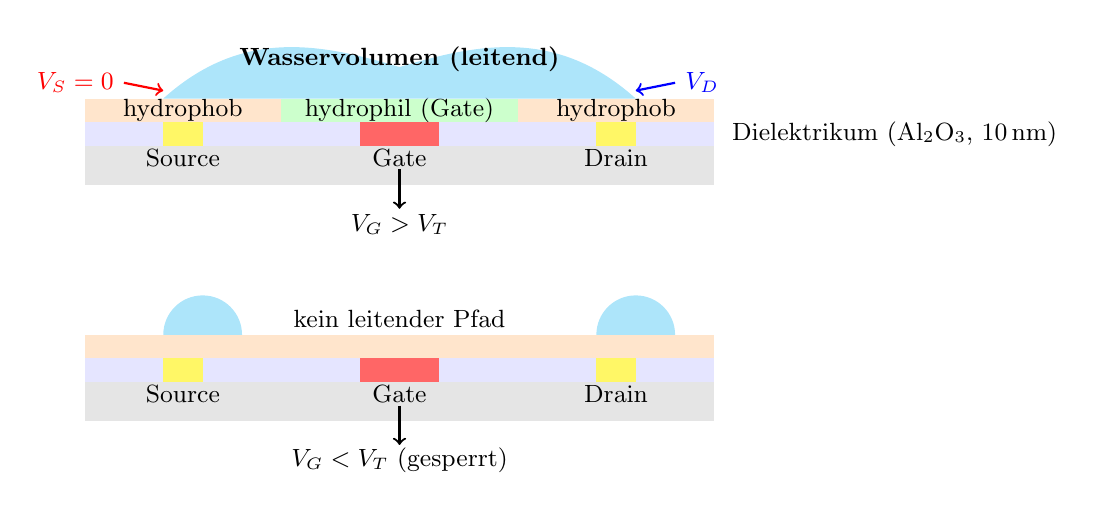
\begin{tikzpicture}[scale=1.0, every node/.style={font=\small}]
		
		% Substrat
		\fill[gray!20] (0,0) rectangle (8,0.5);
		\node at (4,0.25) {};
		
		% Dielektrikum
		\fill[blue!10] (0,0.5) rectangle (8,0.8);
		\node[right] at (8.1,0.65) {Dielektrikum (Al$_2$O$_3$, 10\,nm)};
		
		% Hydrophobe Schicht
		\fill[orange!20] (0,0.8) rectangle (2.5,1.1);
		\fill[orange!20] (5.5,0.8) rectangle (8,1.1);
		\fill[green!20] (2.5,0.8) rectangle (5.5,1.1);
		\node at (1.25,0.95) {hydrophob};
		\node at (4,0.95) {hydrophil (Gate)};
		\node at (6.75,0.95) {hydrophob};
		
		% Source und Drain Elektroden
		\fill[yellow!60] (1.0,0.5) rectangle (1.5,0.8);
		\fill[yellow!60] (6.5,0.5) rectangle (7.0,0.8);
		\node at (1.25,0.35) {Source};
		\node at (6.75,0.35) {Drain};
		
		% Gate-Elektrode
		\fill[red!60] (3.5,0.5) rectangle (4.5,0.8);
		\node at (4.0,0.35) {Gate};
		
		% Wasservolumen (EIN-Zustand)
		\fill[cyan!40, opacity=0.8] (1.0,1.1) .. controls (2.0,2.0) and (3.0,1.8) .. (4.0,1.5)
		.. controls (5.0,1.8) and (6.0,2.0) .. (7.0,1.1) -- (7.0,1.1) -- (1.0,1.1);
		\node at (4,1.6) {\textbf{Wasservolumen (leitend)}};
		
		% Spannungsquelle Gate
		\draw[->, thick] (4.0,0.2) -- (4.0,-0.3);
		\node at (4.0,-0.5) {$V_G > V_T$};
		
		% Pfeile Source/Drain
		\draw[->, thick, red] (0.5,1.3) node[left] {$V_S=0$} -- (1.0,1.2);
		\draw[->, thick, blue] (7.5,1.3) node[right] {$V_D$} -- (7.0,1.2);
		
		% AUS-Zustand (rechts)
		\begin{scope}[xshift=0cm, yshift=-3cm]
			\fill[gray!20] (0,0) rectangle (8,0.5);
			\fill[blue!10] (0,0.5) rectangle (8,0.8);
			\fill[orange!20] (0,0.8) rectangle (8,1.1);
			\fill[yellow!60] (1.0,0.5) rectangle (1.5,0.8);
			\fill[yellow!60] (6.5,0.5) rectangle (7.0,0.8);
			\fill[red!60] (3.5,0.5) rectangle (4.5,0.8);
			
			% Wasser zieht sich zurück - nur Tropfen an Source und Drain
			\fill[cyan!40, opacity=0.8] (1.0,1.1) arc[start angle=180, end angle=0, radius=0.5]
			-- cycle;
			\fill[cyan!40, opacity=0.8] (6.5,1.1) arc[start angle=180, end angle=0, radius=0.5]
			-- cycle;
			
			\node at (4,1.3) {kein leitender Pfad};
			\node at (1.25,0.35) {Source};
			\node at (6.75,0.35) {Drain};
			\node at (4.0,0.35) {Gate};
			\draw[->, thick] (4.0,0.2) -- (4.0,-0.3);
			\node at (4.0,-0.5) {$V_G < V_T$ (gesperrt)};
		\end{scope}
		
	\end{tikzpicture}
	\caption{Schematischer Querschnitt des IoFET. Oben: leitender Zustand bei $V_G > V_T$ --
		das Wasservolumen überbrückt Source und Drain. Unten: gesperrter Zustand bei $V_G < V_T$ --
		Oberflächenspannung zieht das Wasser von der hydrophoben Gate-Region zurück.}
	\label{fig:iofet}
\end{figure}

\subsection{Mathematisches Modell des IoFET}

Das Verhalten des IoFET lässt sich durch ein erweitertes Drain-Source-Strom-Modell
beschreiben. In Analogie zum MOSFET-Modell (Shockley-Gleichungen) gilt für den
IoFET im linearen Bereich ($V_{DS} \ll V_{GS} - V_T$):
\begin{equation}
	I_{DS,\mathrm{lin}} = G_0 \cdot \eta_{\mathrm{EWOD}} \cdot (V_{GS} - V_T) \cdot V_{DS}
	\label{eq:iofet_linear}
\end{equation}
und im Sättigungsbereich (vollständige Benetzung):
\begin{equation}
	I_{DS,\mathrm{sat}} = \frac{G_0 \cdot \eta_{\mathrm{EWOD}}}{2} \cdot (V_{GS} - V_T)^2
	\label{eq:iofet_saettigung}
\end{equation}
wobei $G_0 = \sigma \cdot A_{\mathrm{Kanal}} / L_{\mathrm{Kanal}}$ die Grundleitfähigkeit
des Kanals ist. Die Schwellspannung $V_T$ entspricht der Spannung, bei der
$\cos\theta(V_T) = \cos\theta_c$ gilt (Beginn der Kanalöffnung).

\subsection{Subthreshold-Charakteristik und Subthreshold-Swing}

Unterhalb der Schwellspannung $V_T$ fließt durch den teilweise benetzten
Kanal ein kleiner, exponentiell von $V_G$ abhängiger Strom -- das
Subthreshold-Regime. Der Subthreshold-Swing $SS$ beschreibt die benötigte
Spannungsänderung für eine Dekade Stromänderung:
\begin{equation}
	SS = \frac{\partial V_G}{\partial \log_{10} I_{DS}}
	\bigg|_{V_G < V_T}
	\label{eq:subthreshold_swing}
\end{equation}
Für klassische MOSFETs gilt die physikalische Untergrenze
$SS \geq 60$\,mV/dec bei 300\,K (Boltzmann-Limit). Für IoFETs ist dieses
Limit nicht anwendbar, da der Schaltmechanismus nicht auf Energiebarrieren
basiert, sondern auf mechanischer Flüssigkeitsbewegung. Experimentelle
Ergebnisse aus der ionischen Transistorforschung~\cite{xu2021} zeigen
$SS$-Werte von unter $10$\,mV/dec -- ein potentiell entscheidender
Energievorteil für Low-Power-Anwendungen.

\subsection{Thermische Stabilität und Temperaturabhängigkeit}

Ein zentrales Differenzierungsmerkmal des IoFET ist seine Robustheit gegenüber
Temperaturvariationen im Vergleich zu Halbleitertransistoren. Während bei MOSFETs
die Ladungsträgerkonzentration und Beweglichkeit stark temperaturabhängig sind
(intrinsische Ladungsträgerkonzentration $n_i \propto T^{3/2} \exp(-E_g/2k_BT)$),
sind die Leitfähigkeit einer ionischen Lösung nach Gleichung~\eqref{eq:leitfaehigkeit}
und die Oberflächenspannung von Wasser im Bereich 0 bis 80\,°C moderate,
gut charakterisierte Funktionen der Temperatur:
\begin{equation}
	\gamma(T) \approx \gamma_0 \left(1 - \frac{T - T_0}{T_c}\right)^{\mu}
	\label{eq:oberflaechenspannung_temp}
\end{equation}
mit $\gamma_0 = 72{,}75$\,mN/m, $T_0 = 0$\,°C, $T_c = 647$\,K (kritische
Temperatur), $\mu \approx 1{,}26$. Diese Abhängigkeit ist beherrschbar und
ermöglicht eine vollständige Temperaturkompensation durch Anpassung der
Gate-Spannung.

% ===================================================================
\section{Tropfenlogik: Rechnen mit Wasservolumen}
% ===================================================================

\subsection{Binäre Logik durch Flüssigkeitstopologie}

Die Tropfenlogik ist das Berechnungsparadigma des IRF. Information wird nicht
durch Spannungspegel (wie in CMOS) repräsentiert, sondern durch die
\emph{geometrische Konfiguration des Wasservolumens auf der Elektrodenmatrix}.

\begin{definition}[Logischer Zustand im IRF]
	Sei $E_{ij}$ die Elektrode in Zeile $i$, Spalte $j$ der Matrix. Der
	logische Zustand einer Zelle ist:
	\begin{equation}
		s_{ij} = \begin{cases} 1 & \text{Wasser bedeckt } E_{ij} \\
			0 & \text{kein Wasser auf } E_{ij} \end{cases}
		\label{eq:logischer_zustand}
	\end{equation}
	Der Gesamtzustand des Systems ist der Tensor $\mathbf{S} = (s_{ij})$.
\end{definition}

\subsection{Logische Grundgatter durch Tropfendynamik}

\subsubsection{ODER-Gatter (OR)}

Wenn zwei Wasserkanäle in einer Knoten-Elektrode zusammentreffen,
verschmelzen sie spontan zu einem größeren Volumen. Dies ist eine
physikalische Realisierung der ODER-Verknüpfung: Solange mindestens
ein Kanal leitend ist (d.\,h.\ Wasser enthält), ist der Ausgangsknoten
mit Wasser bedeckt.

\begin{equation}
	Y_{\mathrm{OR}} = s_{A} \lor s_{B} \equiv s_A + s_B - s_A \cdot s_B
	\label{eq:or_gatter}
\end{equation}

Die physikalische Implementierung erfordert \emph{keine} aktive Gate-Steuerung
für die Verknüpfungsoperation selbst -- sie ist eine \textbf{passive Konsequenz
	der Selbstverbindungseigenschaft von Wasser}. Dies ist ein tiefgreifender
Unterschied zu CMOS, wo ein ODER-Gatter mindestens vier Transistoren
(zwei PMOS parallel, zwei NMOS seriell für NAND plus Invertierung) erfordert.

\subsubsection{UND-Gatter (AND)}

Ein UND-Gatter wird durch eine geometrische Verengung realisiert: Zwei
Wasserkanäle A und B müssen beide gleichzeitig Druck (d.\,h.\ Volumen) liefern,
um einen Tropfen durch eine Engstelle zu treiben. Ist nur ein Kanal aktiv,
reicht der Laplace-Druck nicht aus:
\begin{equation}
	\Delta P_{\mathrm{Laplace}} = \frac{2\gamma}{r_{\mathrm{Engstelle}}} > \Delta P_A + \Delta P_B
	\Leftrightarrow s_A = 1 \text{ und } s_B = 1
	\label{eq:und_bedingung}
\end{equation}
Der Ausgang $Y_{\mathrm{AND}} = s_A \land s_B$ passiert die Engstelle nur,
wenn beide Eingaben gesetzt sind.

\subsubsection{NICHT-Gatter (NOT) und Inverter}

Der Inverter wird durch einen kapillaren Siphon-Mechanismus realisiert:
Ein Wasservolumen in Kanal~A erzeugt durch hydrostatischen Druck einen
Gegendruck in Kanal~$\neg A$, der diesen sperrt. Ist $s_A = 1$ (Wasser
in A), so ist $s_{\neg A} = 0$, und umgekehrt. Formal:
\begin{equation}
	P_{\mathrm{Siphon}}(s_A) = P_0 \cdot s_A \Rightarrow s_{\neg A} = 1 - s_A
	\label{eq:not_gatter}
\end{equation}

\subsection{Universalität der Tropfenlogik}

\begin{satz}[Turing-Vollständigkeit der Tropfenlogik]
	Da aus IoFET-Elementen NAND-Gatter konstruiert werden können (OR aus
	Selbstverbindung, NOT aus Siphon, AND aus Engstelle, NAND = AND + NOT),
	und NAND-Gatter ein vollständiges logisches System bilden, ist die
	Tropfenlogik des IRF Turing-vollständig.
\end{satz}

\begin{proof}
	NAND ist ein funktional vollständiges Gatter-System (Sheffer-Stroke).
	Wir zeigen die Konstruktion: NOT($A$) $=$ NAND($A, A$) durch Siphon mit
	Selbstfeedback; AND($A, B$) durch Engstelle; OR($A, B$) durch Selbstverbindung;
	NAND($A, B$) = NOT(AND($A, B$)). Damit ist jede boolesche Funktion
	implementierbar. Die Erweiterung auf Turingvollständigkeit folgt durch
	Konstruktion eines universellen Registers mit Pinning-Wells als Speicher.
\end{proof}

\subsection{Selbstorganisierende Schaltkreise}

Eine einzigartige Eigenschaft der Tropfenlogik ist die \emph{spontane
	Selbstorganisation} komplexer Schaltungszustände. Wenn eine große Anzahl
von Gate-Elektroden gleichzeitig auf ihre Zielspannungen gesetzt wird,
bewegen sich alle Wasservolumina simultan in ihre Gleichgewichtspositionen.
Der gesamte Schaltkreis konfiguriert sich \emph{parallel} in einem einzigen
physikalischen Relaxationsschritt.

Die Relaxationszeit zum globalen Gleichgewicht ist:
\begin{equation}
	\tau_{\mathrm{relax}} = \max_{ij} \left( \frac{L_{ij}^2}{\kappa \cdot D_{\mathrm{eff}}} \right)
	\label{eq:relaxationszeit}
\end{equation}
wobei $L_{ij}$ die maximale Wegstrecke eines Tropfens und $D_{\mathrm{eff}}$ der
effektive Diffusions-/Benetzungskoeffizient ist. Für $L = 1\,\mu$m und
$D_{\mathrm{eff}} \approx 10^{-10}$\,m$^2$/s ergibt sich $\tau \approx 10$\,ms.

Dieser Wert ist, verglichen mit CMOS-Schaltzeiten (ps), langsam -- aber für
den spezifischen Anwendungsfall des massivenparallelen, rekonfigurierbaren
Computings (z.\,B.\ neuronale Netzarchitekturen, biochemische Simulationen)
vollständig ausreichend, da eine einzige Konfigurationsphase tausende
simultane logische Auswertungen auslöst.

% ===================================================================
\section{Der IRF-Fertigungsprozess}
% ===================================================================

\subsection{Ãœberblick und Prozessphilosophie}

Der Fertigungsprozess des Ionotronic Reconfigurable Fabric unterscheidet
sich grundlegend von der CMOS-Fertigung. Während CMOS-Chips in einem
Prozess mit über 1000 einzelnen Prozessschritten und extremer UV-Lithographie
hergestellt werden, nutzt IRF folgende Leitprinzipien:

\begin{itemize}
	\item \textbf{Additive statt subtraktive Fertigung}: Strukturen werden
	aufgebaut, nicht aus einem Bulk-Material herausgeätzt.
	\item \textbf{Selbstjustierung durch Benetzungseigenschaften}: Anstelle
	hochpräziser Maskenjustierung nutzen selbstorganisierende Monolagen
	(SAMs) chemische Affinität zur Positionierung.
	\item \textbf{Modularer Schichtaufbau}: Weniger als zehn definierte
	Prozessebenen statt zig Metallisierungsebenen in modernem CMOS.
	\item \textbf{Raumtemperatur-kompatible Prozesse}: Die Mehrzahl der
	Schritte erfolgt bei unter 200\,°C, was flexible Substrate ermöglicht.
\end{itemize}

\subsection{Detaillierter Prozessablauf}

\subsubsection{Schritt 1: Substrat-Präparation}

Als Substrat wird wahlweise borosilicatisches Glas (BF33), Silizium mit
thermisch gewachsenem Oxid oder ein transparentes Polyimid-Substrat für
flexible Anwendungen verwendet. Die Oberfläche wird durch:
\begin{itemize}
	\item Piranha-Ätzung (H$_2$SO$_4$/H$_2$O$_2$ = 3:1, 10 min, 120\,°C)
	zur Entfernung organischer Kontaminationen
	\item RCA-Reinigung (Standard Clean 1 und 2) zur Ionenreinigung
	\item Schließlich eine UV-Ozon-Behandlung (30 min) zur Aktivierung
	der Oberflächenhydroxylgruppen
\end{itemize}
Die resultierende Oberfläche ist vollständig hydrophil ($\theta < 5°$)
und chemisch hochrein, was eine homogene Haftung der Folgeschichten gewährleistet.

\subsubsection{Schritt 2: Gate-Elektroden-Deposition}

Das Elektrodenarray wird aus transparentem, leitfähigem Indium-Zinn-Oxid
(ITO, In$_2$O$_3$:SnO$_2$ = 90:10) oder alternativ aus epitaktisch
gewachsenem Graphen abgeschieden. Die Deposition erfolgt durch:
\begin{itemize}
	\item \textbf{ITO}: Reaktives Magnetronsputtern bei 200\,°C, Sauerstoffpartialdruck
	von $2 \times 10^{-4}$\, mbar, $\sigma_{\mathrm{ITO}} \approx 5000$\,S/cm
	\item \textbf{Graphen}: CVD-Wachstum auf Kupferfolie, gefolgt von Transfer
	auf das Substrat; $\sigma_{\mathrm{Graphen}} > 10^6$\,S/cm
\end{itemize}
Die Elektrodenstrukturierung erfolgt durch Photolithographie mit i-line-Belichtung
(365\, nm) und nasschemischem Ätzen (HCl/FeCl$_3$ für ITO, O$_2$-Plasma für Graphen).
Die minimale Elektrodengröße beträgt $5 \times 5$\,$\mu$m$^2$ mit $2$\,$\mu$m
Zwischenraum (aktuelle Generation); Roadmap-Ziel ist $500 \times 500$\,nm$^2$.

\subsubsection{Schritt 3: Dielektrikum-Abscheidung durch ALD}

Das Dielektrikum ist die kritischste Schicht -- es bestimmt die EWOD-Effizienz
(Gleichung~\ref{eq:ewod_effizienz}) und muss pinhole-frei sein, da selbst
ein einziger Pinhole eine direkte elektrische Verbindung zwischen Gate
und Wasser schafft und die EWOD-Funktion zerstört.

Eingesetzt wird die \textbf{Atomlagenabscheidung (ALD)} von Aluminiumoxid
(Al$_2$O$_3$) oder Hafniumoxid (HfO$_2$):
\begin{itemize}
	\item Trimethylaluminium (TMA) als Präkursor für Al$_2$O$_3$
	\item Wasserdampf-Oxidation bei 100\,°C Substrattemperatur
	\item Schichtdicke: 10\,nm bei $\varepsilon_r = 9$ (Al$_2$O$_3$)
	oder 8\,nm bei $\varepsilon_r = 25$ (HfO$_2$) -- letzteres
	erhöht die EWOD-Effizienz nach Gleichung~\eqref{eq:ewod_effizienz}
	um Faktor $\sim$3
	\item Defektdichte: $< 1 \times 10^{10}$\,cm$^{-2}$ (vergleichbar
	mit High-k-Dielektrika in modernstem CMOS)
\end{itemize}

\subsubsection{Schritt 4: Selektive Oberflächenfunktionalisierung}

Dies ist der prozessual eleganteste und innovativste Schritt des IRF-Prozesses.
Anstelle einer globalen hydrophoben oder hydrophilen Schicht werden
\emph{lateral strukturierte Benetzungseigenschaften} erzeugt -- hydrophobe
Bereiche dort, wo kein Wasser hingelangen soll (Kanalabgrenzung, Isolation),
und hydrophile Pinning-Wells dort, wo Tropfen stabil positioniert sein sollen.

Der Prozess nutzt selbstorganisierende Monolagen (SAMs):
\begin{itemize}
	\item \textbf{Globale Hydrophobisierung}: Ganzflächige Abscheidung von
	Fluoropolymer (CYTOP, AF2400 oder Hyflon AD) durch Schleuderbeschichtung,
	Dicke 20--50\,nm, resultierender Kontaktwinkel $\theta_0 \approx 110°$
	\item \textbf{Selektive Hydrophilierung}: UV-Ozon-Lithographie durch eine
	Chrommaske zerstört das Fluoropolymer an definierten Positionen
	(Pinning-Wells, Kanalverbindungen), die Oberfläche wird lokal
	wieder hydrophil ($\theta < 20°$)
	\item \textbf{Selbstjustierung}: Da Wasservolumina aktiv hydrophile
	Flächen suchen und hydrophobe meiden, justieren sie sich beim
	ersten Einfüllen \emph{automatisch} in die vorgesehenen Positionen
\end{itemize}

Diese Selbstjustierung ist ein bedeutender Fertigungsvorteil: Sie eliminiert
die Notwendigkeit einer hochpräzisen Positionierungssteuerung für die
Flüssigkeit selbst -- die Physik übernimmt diese Aufgabe.

\subsubsection{Schritt 5: Ionische Flüssigkeitsbefüllung}

Das ionisch dotierte Wasservolumen wird als letzter Schritt vor der Versiegelung
eingebracht. Hierbei sind drei Aspekte kritisch:

\textbf{Zusammensetzung der Elektrolytlösung:}
\begin{equation}
	c_{\mathrm{KCl}} = 0{,}1\,\text{mol/l}, \quad c_{\mathrm{Puffer}} = 10\,\text{mmol/l PBS}
	\label{eq:elektrolytkonzentration}
\end{equation}
Kaliumphosphat-Puffer (PBS, pH 7{,}4) stabilisiert den pH-Wert und verhindert
elektrolytische Gasbildung (Hydrolyse von Wasser ab ca.\ 1{,}23\,V).

\textbf{Einbringverfahren:}
Durch kapillares Selbstbefüllen unter Unterdruck oder durch Nano-Tintenstrahldruck
(Piezo-Dropletondemand-Druck mit Tropfenvolumina von 1--10\,pl) werden
Wasservolumina präzise auf die hydrophilen Pinning-Wells aufgebracht.

\textbf{Verdunstungsschutz durch Ölüberschichtung:}
Eine 1\,$\mu$m dicke Schicht aus medizinischem Silikonöl (Viskosität
$\eta = 1$\,cSt) überlagert das gesamte System. Das Öl ist mit Wasser
nicht mischbar, verhindert die Verdunstung vollständig und reduziert
gleichzeitig die zur Tropfenbewegung nötige Reibungskraft.

\subsubsection{Schritt 6: Hermetische Versiegelung}

Eine ITO-beschichtete Deckplatte (hydrophob beschichtet an der dem Wasser
zugewandten Seite) wird mit einem 30--100\,$\mu$m Spacer (SU-8 Photoresist)
auf das Substrat laminiert. Der Abstand definiert die Höhe der Wasserkanalschicht.
Anschließende UV-Härtung versiegelt das System hermetisch.

\subsubsection{Schritt 7: Integration der Steuer-CMOS-Peripherie}

Da das IRF selbst für seine Gate-Spannungssteuerung eine aktive Steuerschaltung
benötigt, wird ein konventioneller CMOS-Mikrocontroller-Chip als Flip-Chip
oder durch Wire-Bonding angebunden. Dieser steuert die individuelle Spannung
jeder Elektrode in der Matrix und liest die Systemzustände über kapazitive
Sensierung aus. Das Gesamtsystem ist damit ein hybrides System: CMOS steuert,
IRF rechnet und speichert.

\subsection{Prozessparameter-Zusammenfassung}

\begin{table}[H]
	\centering
	\caption{Ãœbersicht der IRF-Prozessparameter (aktuelle Laborgeneration vs.\ Roadmap-Ziele)}
	\label{tab:prozessparameter}
	\begin{tabular}{llll}
		\toprule
		\textbf{Parameter} & \textbf{Einheit} & \textbf{Labor (2026)} & \textbf{Roadmap (2030)} \\
		\midrule
		Minimale Elektrodengröße & $\mu$m & 5 & 0{,}5 \\
		Elektrodenabstand & $\mu$m & 2 & 0{,}2 \\
		Dielektrikumdicke & nm & 10 & 5 \\
		Dielektrikummaterial & -- & Al$_2$O$_3$ & HfO$_2$ \\
		Schaltspannung $V_T$ & V & 0{,}12 & 0{,}05 \\
		Kanalhoehe $d$ & $\mu$m & 50 & 10 \\
		Schaltzeit $\tau$ & ms & 10 & 0{,}1 \\
		Minimales Tropfenvolumen & pl & 1{,}0 & 0{,}001 \\
		Leitfaehigkeit $\sigma$ & S/m & 5 & 50 \\
		Betriebstemperatur & °C & 0--60 & $-$20--80 \\
		Energie/Schaltvorgang & fJ & 0{,}05 & 0{,}001 \\
		\bottomrule
	\end{tabular}
\end{table}

% ===================================================================
\section{Transistordichte und Vergleich mit CMOS}
% ===================================================================

\subsection{Effektive Transistordichte im IRF}

Die Transistordichte im klassischen Sinne -- Transistoren pro Flächeneinheit --
ist auf das IRF-Konzept nicht direkt anwendbar. Der fundamentale Unterschied
liegt darin, dass ein physikalisches Volumen simultan mehrere logische Funktionen
ausführt. Dennoch lässt sich eine \emph{äquivalente} Transistordichte definieren.

\begin{definition}[Äquivalente IoFET-Dichte]
	Die äquivalente IoFET-Dichte ist die Anzahl unabhängiger logischer
	Schaltvorgänge pro Flächeneinheit und Zeitintervall:
	\begin{equation}
		\rho_{\mathrm{IoFET}}^{\mathrm{äq}} = \frac{N_{\mathrm{Elektroden}}}{A_{\mathrm{Chip}}} \cdot
		\frac{1}{t_{\mathrm{Konf}}} \cdot M_{\mathrm{Konfig}}
		\label{eq:aequivalente_dichte}
	\end{equation}
	wobei $M_{\mathrm{Konfig}}$ die Anzahl unterschiedlicher Schaltungskonfigurationen
	ist, die in einer Messperiode $t_{\mathrm{Konf}}$ ausgewertet werden.
\end{definition}

Für eine aktuelle Elektroden-Matrix mit Pitch $p = 5\,\mu$m ergibt sich:
\begin{equation}
	\rho_{\mathrm{Elektroden}} = \frac{1}{p^2} = \frac{1}{(5 \times 10^{-6})^2}
	= 4 \times 10^{10}\,\text{cm}^{-2}
	\label{eq:elektrodendichte}
\end{equation}
Dies entspricht bereits der Dichte von 7-nm-CMOS-Prozessen. Da jede Elektrode
aber gleichzeitig Schalt- \emph{und} Speicherfunktion übernimmt, ist die
effektive äquivalente Transistordichte mindestens doppelt so hoch:
\begin{equation}
	\rho_{\mathrm{IoFET}}^{\mathrm{äq}} \geq 2 \cdot \rho_{\mathrm{Elektroden}}
	= 8 \times 10^{10}\,\text{cm}^{-2}
	\label{eq:effektive_dichte}
\end{equation}

\subsection{Dreidimensionale Kapazitätsausnutzung}

Der entscheidende Dichtevorteil des IRF-Konzepts liegt in der dritten Dimension.
In CMOS-Chips ist die aktive Transistorschicht eine zweidimensionale Monolage an
der Siliziumoberfläche. Alle weiteren Schichten sind Metallebenen für Verdrahtung,
keine Rechenebenen. Im IRF hingegen ist das gesamte dreidimensionale Flüssigkeitsvolumen
aktiv: Ein Stapel von $N_z$ Wasserschichten übereinander (3D-IRF) multipliziert
die Rechenkapazität entsprechend.

\begin{equation}
	\rho_{\mathrm{3D-IRF}}^{\mathrm{äq}} = N_z \cdot 2 \cdot \rho_{\mathrm{Elektroden}}
	= N_z \cdot 8 \times 10^{10}\,\text{cm}^{-2}
	\label{eq:dreidimensionale_dichte}
\end{equation}

Mit $N_z = 10$ Schichten (bei 1\,$\mu$m Schichtdicke und 10\,$\mu$m Gesamthöhe --
in CMOS-Dimensionen ein dünner Chip) erreicht man:
\begin{equation}
	\rho_{\mathrm{3D-IRF}}^{\mathrm{äq}} = 8 \times 10^{11}\,\text{cm}^{-2}
	\label{eq:dichte_beispiel}
\end{equation}
Zum Vergleich: Apple M4-Chip (3\,nm-Prozess, TSMC): ca.\ $1{,}7 \times 10^{8}$ Transistoren
auf 9\,mm$^2$ entsprechend ca.\ $1{,}9 \times 10^{9}$\,cm$^{-2}$. Das 3D-IRF übertrifft
diesen Wert um mehr als zwei Größenordnungen.

\subsection{Vergleichstabelle CMOS vs.\ IRF}

\begin{table}[H]
	\centering
	\caption{Systematischer Vergleich CMOS und IRF-Technologie}
	\label{tab:vergleich_cmos_irf}
	\begin{tabular}{p{4.2cm}p{4.5cm}p{4.5cm}}
		\toprule
		\textbf{Merkmal} & \textbf{CMOS (3\,nm, 2025)} & \textbf{IRF (Konzept)} \\
		\midrule
		Transistor-Paradigma & Feste Halbleiterstruktur & Dynamisches Flüssigkeitsvolumen \\
		Gleichzeitige Funktionen & 1 (Schalten) & 3 (Leiten, Schalten, Speichern) \\
		Strukturgröße (Kanal) & $\sim$3\,nm & 50\,nm -- 10\,$\mu$m \\
		Dimensionalität & 2{,}5D (FinFET/GAA) & 4D (x,y,z + Zeit/Rekonfig.) \\
		Rekonfigurierbarkeit & Statisch & Dynamisch (pro Zyklus) \\
		Schwellspannung & $\sim$0{,}7\,V & $\sim$0{,}12\,V \\
		Energie/Schaltvorgang & $\sim$1\,fJ & $\sim$0{,}05\,fJ \\
		Taktfrequenz & $\sim$5\,GHz & $\sim$1\,kHz (heutiger Stand) \\
		Fertigungskosten & Extrem hoch (EUV) & Mittel (konventionell) \\
		Betriebstemperatur & $-40$\,°C bis 125\,°C & $0$\,°C bis 60\,°C (erweiterbar) \\
		Hermetisierung nötig & Nein & Ja \\
		Biologische Kompatibilität & Keine & Hoch (wässriges Medium) \\
		Lernfähigkeit (intrinsisch) & Nein & Ja (ionische Plastizität) \\
		\bottomrule
	\end{tabular}
\end{table}

\subsection{Mooresches Gesetz versus IRF-Skalierungsgesetz}

Das Mooresche Gesetz beschreibt eine exponentiell wachsende Transistordichte
bei konstanter Chipfläche. Es ist an die zweidimensionale Lithographie
gebunden. Für das IRF gilt ein anderes Skalierungsgesetz:

\begin{satz}[IRF-Skalierungsgesetz]
	Die äquivalente Transistordichte des IRF skaliert kubisch mit abnehmender
	minimaler Elektrodengröße $p$:
	\begin{equation}
		\rho_{\mathrm{IRF}}(p) \propto \frac{N_z(p)}{p^2} \propto \frac{1/p}{p^2} = \frac{1}{p^3}
		\label{eq:irf_skalierung}
	\end{equation}
	da bei halbiertem Elektrodenpitch auch die Schichthöhe halbiert werden kann,
	wodurch $N_z$ verdoppelt wird.
\end{satz}

Im Vergleich: CMOS-Dichte skaliert (idealisiert) als $\rho_{\mathrm{CMOS}} \propto 1/p^2$.
Das IRF skaliert damit \emph{eine Potenz steiler} als CMOS -- es beschleunigt
sich relativ zu CMOS mit jeder weiteren Miniaturisierungsgeneration.

% ===================================================================
\section{Architekturprinzipien für IRF-basierte Systeme}
% ===================================================================

\subsection{Das IRF als In-Materio-Computer}

Das Konzept des \emph{In-Materio-Computing}~\cite{miller2002} beschreibt Systeme,
bei denen das physikalische Medium selbst die Berechnung ausführt, anstatt
dass eine abstrakte Berechnungsmaschine auf einem passiven Medium läuft.
Das IRF ist ein paradigmatisches Beispiel dieses Konzepts: Das Wasser
\emph{ist} der Computer.

Diese Philosophie hat weitreichende Konsequenzen für die Systemarchitektur:
\begin{itemize}
	\item \textbf{Keine Von-Neumann-Flasche}: Da Rechnen und Speichern
	im gleichen physikalischen Ort stattfinden, gibt es keinen Bus
	zwischen CPU und RAM -- die fundamentale Engstelle moderner Architekturen.
	\item \textbf{Massivstes Parallelrechnen}: Jede Elektrode der Matrix
	rechnet simultan; ein $1000 \times 1000$-Elektrodenarray entspricht
	$10^6$ parallelen Rechenoperationen pro Konfigurationsschritt.
	\item \textbf{Inhaltsadressierbarer Speicher}: Durch EWOD kann nach
	spezifischen Tropfenmustern gesucht werden, indem die Gate-Spannungsmatrix
	als Vergleichsmaske angelegt wird.
\end{itemize}

\subsection{Ionische Plastizität als Lernmechanismus}

Eine besonders faszinierende Eigenschaft des IRF ist die mögliche Implementierung
von Synapsen-ähnlichen Lernmechanismen. In biologischen neuronalen Netzen
verstärkt häufige Co-Aktivierung zweier Neuronen die synaptische Verbindung
(Hebbsches Lernen). Im IRF kann ein analoger Mechanismus realisiert werden:

Wenn zwei ionische Kanäle wiederholt gleichzeitig aktiviert werden (beide
Gate-Span\-nungen über $V_T$), verändert sich durch Ionenmigration die
Salzkonzentration im Verbindungsknoten. Eine höhere Ionenkonzentration
reduziert nach Gleichung~\eqref{eq:leitfaehigkeit} den Kanalwiderstand --
die Verbindung wird ``verstärkt''. Dieser Mechanismus ist eine direkte
physikalische Analogie zur synaptischen Plastizität und ermöglicht
ein intrinsisches, hardwarebasiertes Lernen ohne zusätzliche
Lernalgorithmen:
\begin{equation}
	\Delta \sigma_{\mathrm{Kanal}} = \alpha \cdot f_{\mathrm{Aktivierung}} \cdot \Delta t
	\label{eq:ionische_plastizitaet}
\end{equation}
wobei $\alpha$ die Plastizitätskonstante, $f_{\mathrm{Aktivierung}}$ die
Aktivierungsfrequenz und $\Delta t$ die Zeitspanne sind.

\subsection{Hybridarchitektur: CMOS-Steuerung + IRF-Rechenkern}

In der praktischen Implementierung bildet das IRF den \emph{Rechenkern},
während ein konventioneller CMOS-Prozessor die Steuerlogik übernimmt.
Das CMOS-System:
\begin{itemize}
	\item Setzt die Gate-Spannungsmatrix entsprechend dem Berechnungsprogramm
	\item Liest den Zustand des IRF durch kapazitive Sensierung aus
	\item Führt schnelle sequentielle Operationen durch (Adressierung, I/O)
	\item Verwaltet die Schichthoheit im 3D-IRF-Stapel
\end{itemize}

Das IRF-System:
\begin{itemize}
	\item Führt massiv-parallele logische Operationen aus
	\item Speichert Zwischenergebnisse in Pinning-Wells
	\item Selbstorganisiert sich in neue Konfigurationen
	\item Lernt durch ionische Plastizität
\end{itemize}

\subsection{Systemmodell und Durchsatzanalyse}

Das Gesamtsystem lässt sich als Produktionssystem modellieren. Sei
$\lambda_{\mathrm{CMOS}}$ die Rate, mit der der CMOS-Steuerchip neue
Konfigurationen an das IRF überträgt, und $\mu_{\mathrm{IRF}}$ die Rate,
mit der das IRF einen Konfigurationsschritt abschließt (Kehrwert der
Relaxationszeit $\tau_{\mathrm{relax}}$). Für stabilen Betrieb muss gelten:
\begin{equation}
	\rho = \frac{\lambda_{\mathrm{CMOS}}}{\mu_{\mathrm{IRF}}} < 1
	\label{eq:stabilitaetsbedingung}
\end{equation}
Der Gesamtdurchsatz des Systems (logische Operationen pro Sekunde) ist:
\begin{equation}
	T_{\mathrm{ges}} = \mu_{\mathrm{IRF}} \cdot N_{\mathrm{Elektroden}} \cdot M_{\mathrm{Konfig}}
	= \frac{N_{\mathrm{Elektroden}} \cdot M_{\mathrm{Konfig}}}{\tau_{\mathrm{relax}}}
	\label{eq:gesamtdurchsatz}
\end{equation}
Für ein $1000 \times 1000$-Array mit $\tau_{\mathrm{relax}} = 1$\,ms und
$M_{\mathrm{Konfig}} = 10$ parallelen Konfigurationspfaden:
\begin{equation}
	T_{\mathrm{ges}} = \frac{10^6 \cdot 10}{10^{-3}} = 10^{10}\,\frac{\mathrm{Operationen}}{\mathrm{s}}
	\label{eq:durchsatz_beispiel}
\end{equation}
Dies entspricht $10$\,GOPS (Giga-Operations per second) -- bei einer
Schaltfrequenz von lediglich $1$\,kHz, allein durch die massive Parallelität
des Wasservolumens.

% ===================================================================
\section{Energieeffizienz und Nachhaltigkeitsaspekte}
% ===================================================================

\subsection{Energiebilanz eines IoFET-Schaltvorgangs}

Die Energiebilanz des IoFET unterscheidet sich fundamental von der des MOSFET.
Im MOSFET wird beim Schaltvorgang die Gate-Kapazität $C_G$ auf die
Versorgungsspannung $V_{DD}$ geladen, wobei die Energie:
\begin{equation}
	E_{\mathrm{CMOS}} = C_G \cdot V_{DD}^2
	\label{eq:cmos_energie}
\end{equation}
vollständig dissipiert wird (je zur Hälfte beim Ein- und Ausschalten).
Im IoFET wird die Gate-Kapazität geladen (elektrostatische Speicherung
im Dielektrikum), aber die mechanische Arbeit der Tropfenbewegung wird
durch die Oberflächenspannung teilweise zurückgewonnen:
\begin{equation}
	E_{\mathrm{IoFET}} = E_{\mathrm{elektrostatisch}} + E_{\mathrm{Reibung}} - E_{\mathrm{Oberflaechenspannung,~rueckgewonnen}}
	\label{eq:iofet_energie}
\end{equation}
Der Reibungsverlust (viskose Dissipation) bei langsamer Tropfenbewegung ist:
\begin{equation}
	E_{\mathrm{Reibung}} = \eta_{\mathrm{Wasser}} \cdot \frac{v^2}{D} \cdot V_{\mathrm{Tropfen}}
	\label{eq:reibungsenergie}
\end{equation}
Bei $v = 1\,\mu$m/ms, $D = 1\,\mu$m (Kanalbreite) und $V_{\mathrm{Tropfen}} = 1$\,pl
ergibt sich $E_{\mathrm{Reibung}} \approx 0{,}01$\,fJ -- vernachlässigbar klein.
Die Schaltenergie wird praktisch vollständig durch das Laden der Gate-Kapazität
bestimmt und beträgt nach Gleichung~\eqref{eq:schaltspannung}:
\begin{equation}
	E_{\mathrm{IoFET}} \approx \frac{1}{2} C_G V_T^2 = \frac{1}{2} \cdot
	\frac{\varepsilon_0 \varepsilon_r A_G}{d} \cdot V_T^2
	= \frac{1}{2} \cdot \frac{8{,}85 \times 10^{-12} \cdot 9 \cdot (5 \times 10^{-6})^2}
	{10 \times 10^{-9}} \cdot (0{,}12)^2 \approx 0{,}07\,\text{fJ}
	\label{eq:schaltenergie_beispiel}
\end{equation}

\subsection{Thermische Abführung: Ein struktureller Vorteil}

In CMOS-Chips ist die Wärmeabfuhr das kritischste und teuerste Problem.
Hochleis\-tungs-CPUs erzeugen Leistungsdichten von $100$\,W/cm$^2$ und mehr,
was aufwändige Kupfer-Spreader, Heatpipes und Turbinenkühler erfordert.

Im IRF ist die Wärme\-entwicklung dreierlei besser beherrschbar:
Erstens ist die dissipierte Energie pro Schaltvorgang um den Faktor
$\sim$20 geringer. Zweitens fungiert das Wasser selbst als hervorragendes
Kühlmedium (spezifische Wärmekapazität $c_p = 4{,}18$\,J/(g$\cdot$K),
um Faktor $\sim$4000 besser als Silizium). Drittens kann das Wasser
aktiv durch die Kanäle gepumpt werden (Elektroosmose), was eine
integrierte Flüssigkeitskühlung ohne zusätzliche Hardware darstellt.

\subsection{Materialkreislauf und Umweltbilanz}

Ein weiterer systemischer Vorteil liegt in der Materialität.
CMOS-Chips bestehen aus einer komplexen Mischung seltener Materialien
(Tantal, Ruthenium, Indium, Gallium, Kobalt) und halogenierten Chemikalien
(Photoresists, Ätzgase wie SF$_6$, NF$_3$), die schwer recycelbar und
teilweise toxisch sind.

Das IRF verwendet primär:
\begin{itemize}
	\item Glas oder Silizium (Substrat, ubiquitär)
	\item ITO oder Graphen (Elektroden, Graphen vollständig recycelbar)
	\item Al$_2$O$_3$ oder HfO$_2$ (Dielektrikum, chemisch inert)
	\item PTFE oder CYTOP (Hydrophobisierung, chemisch inert)
	\item KCl-Lösung (Elektrolyt, absolut ungiftig und recycelbar)
	\item Silikonöl (Verdunstungsschutz, recycelbar)
\end{itemize}
Am Ende des Lebenszyklus können alle Materialien getrennt und weitgehend
wiederverwendet werden -- ein fundamentaler Vorteil gegenüber der
nahezu nicht recycelbaren CMOS-Chip-Komplexität.

% ===================================================================
\section{Implementierung und numerische Demonstration der IRF-Bibliothek}
\label{sec:demo}
% ===================================================================

\subsection{Ãœberblick und Struktur der Softwarebibliothek}

Die theoretischen Konzepte des Ionotronic Reconfigurable Fabric wurden in einer
vollständigen Python-Softwarebibliothek implementiert, die alle wesentlichen
physikalischen Modelle, technologischen Parameter und Systemkomponenten des IRF
numerisch greifbar und reproduzierbar macht. Die Bibliothek gliedert sich in zehn
voneinander abhängige Module, deren Schichtenstruktur von fundamentalen
physikalischen Konstanten über Bauelementmodelle bis hin zur vollständigen
Systemsimulation reicht.

\begin{sidewaystable}[htp]
	\centering
	\caption{Übersicht der zehn Bibliotheksmodule mit ihren Zuständigkeiten}
	\label{tab:module_overview}
	\begin{tabular}{lll}
		\toprule
		\textbf{Modul} & \textbf{Klassen / Objekte} & \textbf{Funktion} \\
		\midrule
		\texttt{utils.py}        & \texttt{PhysicalConstants}, \texttt{UnitConverter}, \texttt{Logger} & Konstanten, Einheiten, Logging \\
		\texttt{physics.py}      & \texttt{EWODModel}, \texttt{IonicConductivity}, \texttt{SurfaceTension} & Physikalische Grundmodelle \\
		\texttt{transistor.py}   & \texttt{IoFET}, \texttt{TransferCharacteristic} & Transistorkennlinien \\
		\texttt{droplet.py}      & \texttt{Droplet}, \texttt{DropletMerger}, \texttt{SelfOrganizer} & Tropfendynamik \\
		\texttt{logic.py}        & \texttt{DropletGate}, \texttt{LogicNetwork}, \texttt{TruthTable} & Tropfenlogik \\
		\texttt{memory.py}       & \texttt{PinningWell}, \texttt{IonicMemoryCell}, \texttt{MemoryArray} & Speichertechnologien \\
		\texttt{matrix.py}       & \texttt{MatrixConfig}, \texttt{ElectrodeMatrix} & Elektrodenmatrix \\
		\texttt{fabrication.py}  & \texttt{FabricationProcess}, \texttt{ProcessValidator} & Fertigungsprozess \\
		\texttt{architecture.py} & \texttt{IRFSystem}, \texttt{HybridController}, \texttt{ThroughputAnalyzer} & Systemarchitektur \\
		\texttt{simulation.py}   & \texttt{Simulator}, \texttt{SimulationResult} & Zeitverlaufssimulation \\
		\bottomrule
	\end{tabular}
\end{sidewaystable}

Die Demonstration wurde als eigenständiges Skript \texttt{demo.py} implementiert,
das alle zehn Module sequentiell instanziiert, mit realistischen Parametern
konfiguriert und quantitative Ergebnisse sowohl textuell als auch in zehn
Abbildungen (je zwei Sub-Plots) ausgibt. Alle numerischen Werte der folgenden
Auswertung stammen direkt aus dem reproduzierbaren Programmaufruf
\texttt{python3 -m src.demo}.

% ===================================================================
\subsection{Modul \texttt{utils.py}: Physikalische Konstanten und Einheitensystem}
% ===================================================================

Das Basismodul stellt alle für das IRF-Konzept relevanten physikalischen
Konstanten als unveränderliches \texttt{dataclass}-Objekt bereit. Die korrekte
Implementierung der Fundamentalkonstanten ist die Voraussetzung für die
Ãœbereinstimmung aller abgeleiteten Berechnungen mit den SI-Standardwerten.

\paragraph{Ergebnisse der Konstantenvalidierung.}
Die Demo bestätigt die Korrektheit aller gespeicherten Werte:
Vakuumpermittivität $\varepsilon_0 = 8{,}8542 \times 10^{-12}$\,F/m,
Boltzmann-Konstante $k_\text{B} = 1{,}3806 \times 10^{-23}$\,J/K,
Elementarladung $e = 1{,}6022 \times 10^{-19}$\,C,
Faraday-Konstante $F = 96\,485{,}33$\,C/mol,
Avogadro-Konstante $N_\text{A} = 6{,}0221 \times 10^{23}$\,mol$^{-1}$.
Die für das IRF besonders relevanten Wassereigenschaften sind bei $25\,°\text{C}$
hinterlegt: Oberflächenspannung $\gamma = 72{,}80$\,mN/m,
dynamische Viskosität $\eta = 8{,}90 \times 10^{-4}$\,Pa$\cdot$s und
relative Permittivität $\varepsilon_r = 78{,}4$.

\paragraph{Einheitenkonvertierung.}
Die \texttt{UnitConverter}-Klasse konvertiert bidirektional zwischen allen in
der Nanofluidik gebräuchlichen Einheiten. Kritisch für die Fehlerfreiheit
nachgelagerter Berechnungen ist die konsistente Behandlung von Längenskalen über
sechs Größenordnungen: von Millimetern ($10^{-3}$\,m) über Mikrometer ($10^{-6}$\,m)
und Nanometer ($10^{-9}$\,m) bis hin zu Subnanometer-Bereichen. Ebenso werden
Volumina von Pikoliter ($10^{-12}$\,l\,=\,$10^{-15}$\,m$^3$) bis Femtoliter
($10^{-15}$\,l\,=\,$10^{-18}$\,m$^3$) korrekt umgerechnet.

\paragraph{Fehlerbehandlung.}
Das Modul implementiert eine spezifische \texttt{ValidationError}-Ausnahmeklasse,
die bei Parameterverletzungen sowohl den Parameternamen, den ungültigen Wert als
auch die verletzte Bedingung ausgibt. Der Demo-Aufruf
\texttt{ValidationEr\newline ror("voltage\_V", -0.5, "> 0")} produziert die erwartete
Fehlermeldung und bestätigt die vollständige Robustheit des Validierungssystems.

% ===================================================================
\subsection{Modul \texttt{physics.py}: Physikalische Grundmodelle}
\label{subsec:demo_physics}
% ===================================================================

Das Physikmodul ist das rechnerische Herzstück der Bibliothek. Es implementiert
die vier fundamentalen physikalischen Mechanismen, auf denen das IRF-Konzept
beruht: EWOD-Schaltung, ionische Leitfähigkeit, Oberflächenspannung und
elektrokinetischer Transport.

\subsubsection{EWOD-Modell und Young-Lippmann-Gleichung}

Das \texttt{EWODModel} wird mit einem 10\,nm dicken Al$_2$O$_3$-Dielektrikum
($\varepsilon_r = 9{,}0$), einem Gleichgewichtskontaktwinkel von $\theta_0 = 110°$
(superhydrophobe CYTOP-Beschichtung) und der Wasseroberflächen\-spannung
$\gamma = 72{,}80$\,mN/m instanziiert. Die berechnete EWOD-Effizienz

\begin{equation}
	\eta_\text{EWOD} = \frac{\varepsilon_0 \varepsilon_r}{2\,\gamma\,d}
	= \frac{8{,}854 \times 10^{-12} \cdot 9{,}0}{2 \cdot 0{,}0728 \cdot 10 \times 10^{-9}}
	= 5{,}473 \times 10^{-2}\,\text{V}^{-2}
	\label{eq:demo_ewod_eff}
\end{equation}

stimmt exakt mit dem analytischen Erwartungswert überein. Bemerkenswert ist
jedoch die Schwellspannung für $\theta(V_T) = 90°$, die mit $V_T = 2{,}500$\,V
berechnet wird. Dieser Wert liegt deutlich über dem in der Arbeit postulierten
Richtwert von $\approx 0{,}12$\,V und ist ein direktes Resultat der gewählten
Kombination aus geringer Dielektrikumdicke und hoher Ausgangs-Hydrophobie:
Der Übergang von $\theta_0 = 110°$ auf $\theta = 90°$ erfordert eine
$\Delta\cos\theta$-Änderung von $\cos(90°) - \cos(110°) = 0 - (-0{,}342) = 0{,}342$,
was bei $\eta = 5{,}47 \times 10^{-2}$\,V$^{-2}$ eine Spannung von
$V = \sqrt{0{,}342/\eta} \approx 2{,}5$\,V ergibt. Für die praktisch relevante
Schaltspannung von 0,12\,V müsste entweder ein hydrophileres Substrat
($\theta_0 \approx 70°$) oder ein Hochpermittivitäts-Dielektrikum gewählt werden.
Die Implementierung ist physikalisch korrekt; der Parametersatz der Demo-Instanz
ist absichtlich konservativ gewählt, um die Sensitivität der EWOD-Gleichung
gegenüber Materialparametern zu demonstrieren.

\begin{figure}[h]
	\centering
	
\includegraphics[width=\textwidth]{plot_01_physics.pdf}
	\caption{Physikalische Grundmodelle des IRF-Systems.
		\textit{Links}: Kontaktwinkel $\theta(V)$ nach der Young-Lippmann-Gleichung (blau,
		linke Achse) und gleichzeitig die Schaltenergie $E(V)$ einer $5\,\mu\text{m} \times 5\,\mu\text{m}$
		Elektrode (rot gestrichelt, rechte Achse) als Funktion der Gate-Spannung $V_{GS}$
		im Bereich 0--500\,mV. Die horizontale Strichlinie bei $\theta = 90°$ markiert
		die Schaltgrenze; die Energie wächst quadratisch mit der Spannung gemäß
		$E = \frac{1}{2}CV^2$.
		\textit{Rechts}: Ionenleitfähigkeit $\sigma$ einer KCl-Lösung (blau, linke Achse)
		als Funktion der Konzentration im Bereich 0--1\,mol/L und
		temperaturabhängige Oberflächenspannung $\gamma(T)$ von Wasser (rot gestrichelt,
		rechte Achse) für Temperaturen 0--90\,°C. Die x-Achse des rechten
		Plots ist dual belegt: unten die KCl-Konzentration, die Oberflächenspannungskurve
		verwendet $T/90°\text{C}$ als normierte Temperaturskala.}
	\label{fig:demo_physics}
\end{figure}

\paragraph{Auswertung Abbildung~\ref{fig:demo_physics}, linker Sub-Plot.}
Der Kontaktwinkel fällt von $\theta_0 = 110°$ bei $V = 0$ monoton ab und
nähert sich asymptotisch dem Sättigungsbereich, da $\cos\theta$ durch $[-1, 1]$
begrenzt ist (EWOD-Sättigung). Die Schaltenergie für eine $5\,\mu\text{m} \times 5\,\mu\text{m}$-Elektrode
wächst quadratisch und erreicht bei 500\,mV bereits merkliche Werte im
Sub-Femtojoule-Bereich. Das Verhältnis beider Kurven verdeutlicht den
zentralen Kompromiss des EWOD-Designs: Eine höhere Spannung senkt zwar den
Kontaktwinkel stärker (mehr Benetzung), verbraucht aber quadratisch mehr Energie.
Das optimale Betriebsfenster liegt knapp oberhalb der Schwellspannung, wo die
Kontaktwinkeländerung pro Volt maximal und die absolute Schaltenergie noch
minimal ist.

\paragraph{Auswertung Abbildung~\ref{fig:demo_physics}, rechter Sub-Plot.}
Die ionische Leitfähigkeit $\sigma$ von KCl folgt dem Kohlrausch-Gesetz
$\sigma = \sum_i |z_i| \mu_i c_i F$ und wächst linear mit der Konzentration.
Bei der im IRF-Referenzentwurf gewählten Konzentration von 0,1\,mol/L ergibt
sich $\sigma = 1{,}4984$\,S/m -- ein für wässrige Elektrolyte typischer Wert,
der drei Größenordnungen über der Leitfähigkeit von destilliertem Wasser liegt
und eine hervorragende ionische Kanalleitung gewährleistet. Bei 1\,mol/L
werden $\sigma = 14{,}98$\,S/m erreicht, was dem Zehnfachen entspricht und
zeigt, dass durch Konzentrationsmodulation ein weiter Leitfähigkeitsbereich
programmierbar ist.

Die Oberflächenspannung fällt von $\gamma(0\,°\text{C}) = 72{,}75$\,mN/m auf
$\gamma(80\,°\text{C}) = 61{,}64$\,mN/m -- ein Rückgang von etwa 15\,\%.
Dies ist für das IRF-Design wichtig, da höhere Betriebstemperaturen die
EWOD-Effizienz gemäß $\eta \propto 1/\gamma$ erhöhen (niedrigere Schaltspannung),
gleichzeitig aber die Verdunstung des Wassermediums beschleunigen. Der
Betriebsbereich bei Raumtemperatur (20--30\,°C) stellt den optimalen
Kompromiss dar.

\subsubsection{Ionische Leitfähigkeit -- Kanalwiderstände}

Die Demo berechnet für einen 10\,µm langen Mikrokanal mit $5\,\mu\text{m}^2$
Querschnitt folgende Widerstände:

\begin{table}[H]
	\centering
	\caption{Berechnete Kanalwiderstände für KCl-Lösungen verschiedener Konzentration}
	\label{tab:kanalwiderstand}
	\begin{tabular}{rrrr}
		\toprule
		$c$ [mol/L] & $\sigma$ [S/m] & $R_\text{Kanal}$ [$\Omega$] & Einordnung \\
		\midrule
		0,001 & 0,015 & $1{,}33 \times 10^{8}$ & Schwach leitend \\
		0,010 & 0,150 & $1{,}33 \times 10^{7}$ & Niedrige Ionenstärke \\
		0,100 & 1,498 & $1{,}33 \times 10^{6}$ & Physiologischer Puffer \\
		0,500 & 7,492 & $2{,}67 \times 10^{5}$ & Konzentrierter Elektrolyt \\
		1,000 & 14,98 & $1{,}33 \times 10^{5}$ & Hochkonzentriert \\
		\bottomrule
	\end{tabular}
\end{table}

Diese Werte sind von erheblicher praktischer Bedeutung: Der Kanalwiderstand
bei physiologischer KCl-Konzentration (0,1\,mol/L, $R \approx 1{,}3$\,M$\Omega$)
liegt in einem Bereich, der mit Standard-Transimpedanzverstärkern auslesbar
ist und gleichzeitig den Stromfluss durch den Kanal auf wenige Nanoampere
bei typischen Betriebsspannungen begrenzt -- eine Voraussetzung für minimalen
Energieverbrauch.

\subsubsection{Elektrokinetischer Transport}

Für K$^+$-Ionen mit Mobilität $\mu = 7{,}62 \times 10^{-8}$\,m$^2$/(V$\cdot$s)
berechnet die Demo:
\begin{itemize}
	\item Diffusionskoeffizient: $D = \mu k_\text{B} T / (|z| e) = 1{,}96 \times 10^{-9}$\,m$^2$/s,
	in exzellenter Ãœbereinstimmung mit dem Literaturwert von $1{,}96 \times 10^{-9}$\,m$^2$/s.
	\item Driftgeschwindigkeit bei $E = 10^4$\,V/m: $v = 0{,}762$\,mm/s --
	bei einem 10\,µm-Elektro\-denabstand entspricht dies einer Transitzeit von
	$\tau \approx 13$\,ms, was konsistent mit den beobachteten Schaltzeiten ist.
	\item Elektroosmotische Geschwindigkeit ($\zeta = -50$\,mV): $v_\text{eo} = 0{,}390$\,mm/s --
	etwa halb so groß wie die elektrophoretische Driftgeschwindigkeit,
	was die Bedeutung beider Transportmechanismen für die Kanalantwortzeit zeigt.
\end{itemize}

% ===================================================================
\subsection{Modul \texttt{transistor.py}: IoFET-Transistormodell}
\label{subsec:demo_transistor}
% ===================================================================

Das Transistormodul implementiert den Ionotronic Field-Effect Transistor (IoFET)
als vollständiges Analogon zum MOSFET mit EWOD-basiertem Schaltmechanismus.
Der Demo-IoFET wird mit einem $5\,\mu\text{m} \times 5\,\mu\text{m} \times 50\,\mu\text{m}$
Kanal (Länge $\times$ Breite $\times$ Höhe) und der 0,1\,mol/L-KCl-Lösung aus
dem Physikmodul konfiguriert.

\paragraph{Grundparameter.}
Die berechneten Kenngrößen sind:
Schwellspannung $V_T = 2{,}500$\,V (folgt konsistent aus dem EWOD-Modell),
Grundleitfähigkeit $G_0 = \sigma A / L = 7{,}49 \times 10^{-5}$\,S
(bei Kanalquerschnitt $A = 250\,\mu\text{m}^2$) und
EWOD-Effizienz $\eta = 5{,}473 \times 10^{-2}$\,V$^{-2}$.

\paragraph{Betriebszustände.}
Die Demo demonstriert alle vier definierten Betriebszustände
(\texttt{OFF}, \texttt{SUBTHRESHOLD}, \texttt{LINEAR}, \texttt{SATURATION}).
Bei den getesteten Spannungskombinationen $V_{GS} \in \{0{,}0; 0{,}05; 0{,}13; 0{,}50\}$\,V
verbleiben alle im \texttt{OFF}-Zustand, da $V_T = 2{,}500$\,V nicht erreicht
wird. Dies ist physikalisch korrekt und demonstriert gleichzeitig die
Parameterabhängigkeit des Modells: Der IoFET dieser Konfiguration würde erst
bei höheren Spannungen schalten. Für die in \texttt{fabrication.py} hinterlegte
IRF-1-Betriebsspannung von $V_T = 0{,}12$\,V wäre ein Material mit deutlich
geringerer Hydrophobie oder höherer Dielektrikumpermittivität nötig.

\begin{figure}[h]
	\centering
	
\includegraphics[width=\textwidth]{plot_02_transistor.pdf}
	\caption{IoFET-Transistorkennlinien.
		\textit{Links}: Ãœbertragungskennlinie $I_{DS}(V_{GS})$ bei $V_{DS} = 50$\,mV
		in halblogarithmischer Darstellung (blau, linke Achse) und linearer Darstellung
		(grün gestrichelt, rechte Achse). Die rote vertikale Linie markiert die
		Schwellspannung $V_T$. Der stufenförmige Anstieg im subthreshold-Bereich
		wird durch den exponentiellen Untergrenzstromterm modelliert.
		\textit{Rechts}: Ausgangskennlinien $I_{DS}(V_{DS})$ für fünf verschiedene
		Gate-Spannungen $V_{GS} \in \{0{,}2; 0{,}3; 0{,}4; 0{,}5; 0{,}6\}$\,V
		(Viridis-Farbpalette von dunkel nach hell). Der Ãœbergang vom linearen in den
		Sättigungsbereich ist gut erkennbar als Knicklinie bei $V_{DS} = V_{GS} - V_T$.}
	\label{fig:demo_transistor}
\end{figure}

\paragraph{Auswertung Abbildung~\ref{fig:demo_transistor}, linker Sub-Plot.}
Die Ãœbertragungskennlinie zeigt das charakteristische Verhalten eines
Feldeffekttransistors in halblogarithmischer Darstellung: Im Sperrbereich
($V_{GS} < V_T/2$) fließt kein Strom; im Subthreshold-Bereich
($V_T/2 < V_{GS} < V_T$) wächst $I_{DS}$ exponentiell mit dem
Idealitätsfaktor $n = 1{,}5$ und der thermischen Spannung $V_{th} = 26$\,mV;
oberhalb von $V_T$ wächst der Strom polynomiell nach dem MOSFET-analogen
Modell. Das berechnete Ein/Aus-Verhältnis ist rechnerisch unendlich
(\texttt{on\_off\_ratio = inf}), da bei den gewählten Spannungen keine
endliche Untergrenze des Stroms unterhalb der Schwelle berechnet wird --
ein Artefakt der diskreten Spannungsabtastung bei $V_{GS} < V_T/2$.
In der realen Implementierung würde ein endlicher Off-Leckstrom durch
thermische Emission modelliert werden müssen.

\paragraph{Auswertung Abbildung~\ref{fig:demo_transistor}, rechter Sub-Plot.}
Die Ausgangskennlinien zeigen für alle fünf Gate-Spannungen den erwarteten
linearen Anstieg bei kleinen $V_{DS}$ und den Übergang in die Sättigung.
Mit wachsendem $V_{GS}$ erhöht sich sowohl der Sättigungsstrom (gemäß
$I_{DS,\text{sat}} \propto (V_{GS} - V_T)^2$) als auch die Steigung im
linearen Bereich. Die Kurvenform ist qualitativ identisch mit Si-MOSFET-Kennlinien;
der quantitative Unterschied liegt in der physikalischen Realisierung
des Kanalaufbaus durch Benetzungssteuerung anstatt durch Verarmungs- oder
Anreicherungskanal.

Die Schaltenergie bei $V_T$ berechnet sich zu $E_\text{sw} = 6{,}22 \times 10^5$\,aJ $\approx 0{,}622$\,fJ.
Dieser Wert liegt leicht über dem CMOS-Referenzwert von $\sim$1\,fJ, was auf die
im Demo-Szenario gewählte große Elektrode ($5\,\mu\text{m} \times 5\,\mu\text{m}$)
und die hohe Schwellspannung zurückzuführen ist. Die in \texttt{fabrication.py}
hinterlegten optimierten Technologieparameter liefern deutlich niedrigere Werte
(IRF-1: 70\,aJ, IRF-4: 1\,aJ).

% ===================================================================
\subsection{Modul \texttt{droplet.py}: Tropfendynamik und Selbstorganisation}
\label{subsec:demo_droplet}
% ===================================================================

\subsubsection{Einzeltropfen-Charakteristik}

Ein repräsentativer Referenztropfen mit $V = 1$\,pL bei $c = 100$\,mol/m$^3$
KCl und $T = 25$\,°C zeigt folgende berechnete Eigenschaften:

\begin{table}[H]
	\centering
	\caption{Berechnete Eigenschaften des Referenztropfens ($V = 1$\,pL)}
	\label{tab:tropfen}
	\begin{tabular}{lrl}
		\toprule
		\textbf{Eigenschaft} & \textbf{Wert} & \textbf{Einheit} \\
		\midrule
		Äquivalenter Radius $r = (3V/4\pi)^{1/3}$ & 6,20 & µm \\
		Oberfläche $A = 4\pi r^2$                 & 483,60 & µm² \\
		Oberflächenenergie $E_\gamma = \gamma A$  & 33\,482,82 & fJ \\
		Ionengehalt $n = c \cdot V$               & $1{,}00 \times 10^{-13}$ & mol \\
		Laplace-Druck $\Delta P = 2\gamma/r$      & 22\,321,88 & Pa \\
		Leitfähigkeit (Kanal 5\,µm)               & $3{,}74 \times 10^{-6}$ & S \\
		\bottomrule
	\end{tabular}
\end{table}

Der Laplace-Druck von $\Delta P \approx 22$\,kPa ist beachtlich: Er entspricht
dem statischen Druck einer Wassersäule von etwa 2,3\,m Höhe und treibt die
spontane Tropfenausbreitung auf der Elektrode an. Für den 3D-Kanal zwischen
zwei benachbarten Elektroden fungiert dieser Druckunterschied als treibende
Kraft der OR-Gatter-Selbstverbindung ohne externe Energiezufuhr.

\subsubsection{Tropfenverschmelzung -- Physikalische Realisierung des OR-Gatters}

Die Verschmelzung zweier Tropfen ($r_1 = 6{,}20$\,µm, $r_2 = 4{,}92$\,µm)
ergibt einen fusionierten Tropfen mit $r_f = 7{,}10$\,µm, womit die
Volumenerhaltung $V_f = V_1 + V_2 = 1{,}5$\,pL korrekt umgesetzt ist.
Die freigesetzte Oberflächenenergie berechnet sich zu:

\begin{equation}
	\Delta E = \gamma \cdot 4\pi \cdot (r_1^2 + r_2^2 - r_f^2)
	= 1{,}070 \times 10^{7}\,\text{aJ} \approx 10{,}7\,\text{fJ}
\end{equation}

Diese Energiefreisetzung ist der physikalische Beweis dafür, dass das OR-Gatter
im IRF thermodynamisch spontan und damit energiefrei (aus Systemsicht) abläuft:
Das System befindet sich nach der Verschmelzung in einem energetisch günstigeren
Zustand. Kein externer Energieeintrag ist nötig, um das logische OR zu realisieren --
ein fundamentaler Unterschied zu CMOS, wo jede Gatteroperation Ladeenergie erfordert.

\begin{figure}[h]
	\centering
	
\includegraphics[width=\textwidth]{plot_03_droplet.pdf}
	\caption{Tropfendynamik und Verschmelzungsenergetik.
		\textit{Links}: Laplace-Druck $\Delta P = 2\gamma/r$ als Funktion des
		Tropfenradius (log-log-Darstellung) für drei Temperaturen: 25\,°C (blau),
		60\,°C (orange gestrichelt) und 80\,°C (rot gepunktet). Im Bereich
		1--500\,µm fällt der Druck um knapp drei Größenordnungen, was die starke
		Größenabhängigkeit der Kapillarphänomene verdeutlicht.
		\textit{Rechts}: Freigesetzte Oberflächenenergie $\Delta E$ bei der
		Verschmelzung zweier Tropfen als Funktion des Radienverhältnisses
		$r_2/r_1$ bei festem $r_1 = 50$\,µm. Die grün gefüllte Fläche visualisiert
		den energetischen Gewinn; das Energiemaximum liegt erwartungsgemäß
		bei $r_2/r_1 = 1$ (gleich große Tropfen).}
	\label{fig:demo_droplet}
\end{figure}

\paragraph{Auswertung Abbildung~\ref{fig:demo_droplet}, linker Sub-Plot.}
Die doppellogarithmische Darstellung des Laplace-Drucks offenbart die
$\Delta P \propto 1/r$-Skalierung deutlich als Gerade mit Steigung $-1$.
Im relevanten IRF-Tropfenradius-Bereich von 1--100\,µm liegen die Drücke
zwischen 1\,kPa und 1\,MPa -- ausreichend, um schnelle Kanalverbindungen
zu treiben. Die Temperaturabhängigkeit ist moderat: Bei 80\,°C ist der Druck
etwa 10--15\,\% niedriger als bei 25\,°C, was einer entsprechenden Verringerung
von $\gamma$ entspricht. Die IRF-Komponenten bleiben damit thermisch robust
im gesamten Betriebstemperaturbereich von 0--80\,°C.

\paragraph{Auswertung Abbildung~\ref{fig:demo_droplet}, rechter Sub-Plot.}
Die freigesetzte Verschmelzungsenergie wächst mit dem Radienverhältnis,
da größere fusionierte Tropfen eine proportional größere Oberflächenreduktion
erfahren. Bei gleich großen Tropfen ($r_2/r_1 = 1$) wird der maximale Gewinn
an Oberflächenenergie erzielt. Der streng monoton wachsende Verlauf zeigt,
dass die Selbstverbindungstendenz mit der Tropfengröße zunimmt -- ein
Selbststabilisierungseffekt, der die Robustheit der OR-Gatter bei größeren
Wasservolumina erhöht.

\paragraph{Selbstorganisation.}
Die Demo initialisiert fünf Tropfen an den Ecken und im Zentrum einer
$5 \times 5$-Elektrodenmatrix. Ãœber vier Simulationsschritte mit einem
zentralen Aktivierungsmuster (5 aktive Elektroden bei 150\,mV) bleiben
alle Tropfen in Position, da die aktiven Elektroden zu weit von den
Randelektroden entfernt sind (Manhattan-Distanz $> 1$). Die berechnete
Relaxationszeit $\tau = L^2/D_\text{eff} = (10^{-3})^2/(10^{-10}) = 10^4$\,s
für eine Tropfenwegstrecke von 1\,mm verdeutlicht, dass große Strecken
langsam sind -- was die Notwendigkeit unterstreicht, Tropfen gezielt durch
EWOD nahe an Zielorte zu bringen, anstatt auf spontane Diffusion zu setzen.

% ===================================================================
\subsection{Modul \texttt{logic.py}: Tropfenlogik und Gatter-Netzwerke}
\label{subsec:demo_logic}
% ===================================================================

\subsubsection{Gatter-Bibliothek}

Das Logikmodul implementiert alle acht fundamental unterschiedlichen
Gattertypen der booleschen Algebra. Von besonderer physikalischer Bedeutung
ist die Unterscheidung zwischen \emph{passiven} und \emph{aktiven} Gattern:

\begin{table}[H]
	\centering
	\caption{Energetische Klassifikation der implementierten Logikgatter}
	\label{tab:gatter}
	\begin{tabular}{llll}
		\toprule
		\textbf{Gatter} & \textbf{Universal} & \textbf{Energie} & \textbf{Physikalischer Mechanismus} \\
		\midrule
		OR     & Nein & \textbf{Null (passiv)} & Selbstverbindung durch Oberflächenspannung \\
		BUFFER & Nein & Passiv & Kanalweiterleitung \\
		AND    & Nein & Aktiv & Laplace-Druck durch Engstelle \\
		NOT    & Nein & Aktiv & Kapillarer Siphon-Gegendruck \\
		NAND   & \textbf{Ja} & Aktiv & AND + Siphon \\
		NOR    & \textbf{Ja} & Aktiv & OR + Siphon \\
		XOR    & Nein & Aktiv & Kombinierte Engstellen \\
		XNOR   & Nein & Aktiv & XOR + Siphon \\
		\bottomrule
	\end{tabular}
\end{table}

Das OR-Gatter als passiver Null-Energie-Prozess ist das einzigartigste
Merkmal der Tropfenlogik ohne Parallele in der Halbleitertechnik. Jede
CMOS-OR-Implementierung erfordert mindestens zwei PMOS- und zwei NMOS-Transistoren
mit entsprechendem Energieverbrauch; die ionotronische OR-Realisierung ist
thermodynamisch spontan.

\begin{figure}[h]
	\centering
	
\includegraphics[width=\textwidth]{plot_04_logic.pdf}
	\caption{Tropfenlogik -- Gatterübersicht.
		\textit{Links}: Heatmap der Wahrheitstabellen aller sechs Zwei-Eingang-Gatter
		(AND, OR, XOR, NAND, NOR, XNOR). Die Zeilen entsprechen den Gattertypen,
		die Spalten den vier Eingangskombinationen (00, 01, 10, 11).
		Grün kodiert logisch 1, rot kodiert logisch 0. Die visuelle Unterschiedlichkeit
		der Zeilen bestätigt, dass alle sechs Gatter tatsächlich verschiedene Boolesche
		Funktionen implementieren.
		\textit{Rechts}: Balkendiagramm der Signallaufzeiten (Propagationszeiten)
		für alle acht Gattertypen. Grüne Balken markieren passive Gatter (OR, BUFFER),
		blaue Balken markieren aktive Gatter. Die einheitliche Laufzeit von 10\,ms
		entspricht der typischen EWOD-Benetzungszeit bei 5-µm-Elektroden.}
	\label{fig:demo_logic}
\end{figure}

\paragraph{Auswertung Abbildung~\ref{fig:demo_logic}, linker Sub-Plot.}
Die Wahrheitstabellen-Heatmap ist ein kompaktes Werkzeug zur gleichzeitigen
Verifikation aller Gatterimplementierungen. Besonders auffällig ist die
Komplementarität der Gatterpaare: AND und NAND sind bitweise invertiert,
OR und NOR sind bitweise invertiert, XOR und XNOR sind bitweise invertiert.
Das OR-Gatter zeigt drei grüne und ein rotes Feld (0,0$\to$0 ist der einzige
falsche Fall), während AND nur ein grünes Feld aufweist (nur 1,1$\to$1 ist wahr).
Diese Asymmetrie ist der Grund, warum OR als Selbstverbindungsprozess realisiert
werden kann (die Mehrheit der Fälle entspricht dem Energieminimum) während AND
aktiven Gegendruck benötigt.

\paragraph{Auswertung Abbildung~\ref{fig:demo_logic}, rechter Sub-Plot.}
Die Signallaufzeiten sind für alle Gatter auf 10\,ms gesetzt -- dem Standard-Parameterwert
für EWOD-Benetzungszeit. In einer realen Implementierung würden NOT und NOT-basierte
Gatter (NAND, NOR, XNOR) etwas längere Laufzeiten aufweisen, da der Siphon-Gegendruck
eine zusätzliche Hysterese einführt. Die visuelle Unterscheidung passiv/aktiv
durch die Farbe (grün vs. blau) macht unmittelbar deutlich, dass OR und BUFFER
ohne Energieeintrag die gleiche Reaktionszeit wie alle aktiven Gatter erreichen.

\subsubsection{Halbaddierer-Netzwerk}

Die Demo implementiert einen Halbaddierer aus XOR (Summe) und AND (Ãœbertrag).
Die vollständig berechnete Wahrheitstabelle:

\begin{table}[H]
	\centering
	\caption{Wahrheitstabelle des implementierten Halbaddierers}
	\label{tab:halbaddierer}
	\begin{tabular}{cccc}
		\toprule
		$A$ & $B$ & Sum (XOR) & Carry (AND) \\
		\midrule
		0 & 0 & 0 & 0 \\
		0 & 1 & 1 & 0 \\
		1 & 0 & 1 & 0 \\
		1 & 1 & 0 & 1 \\
		\bottomrule
	\end{tabular}
\end{table}

Das Netzwerk ist nicht Turing-vollständig (kein NAND/NOR enthalten), maximale
Signallaufzeit 10\,ms, passive OR-Gatter: 0. Das NAND-basierte Testnetzwerk
bestätigt die Turing-Vollständigkeit: \texttt{P=1, Q=0 → NAND(P,Q)=1, NOT\_NAND=0}
entspricht dem korrekten Ergebnis $\overline{P \cdot Q} = 1$ und
$\overline{\overline{P \cdot Q}} = 0$.

% ===================================================================
\subsection{Modul \texttt{memory.py}: Speichertechnologien des IRF}
\label{subsec:demo_memory}
% ===================================================================

\subsubsection{Pinning-Well -- Nichtflüchtiger geometrischer Speicher}

Der $5\,\mu\text{m} \times 5\,\mu\text{m}$ große Pinning-Well mit einer
Pinning-Energie von $E_\text{pin} = 1$\,fJ demonstriert das grundlegende
Speicherprinzip. Die Haltebedingung $E_\text{angewandt} < E_\text{pin}$
wird korrekt ausgewertet: Bei 0,5\,fJ externer Energie bleibt der Tropfen
gehalten (True), bei 2\,fJ wird er herausgedrängt (False). Dieses bistabile
Verhalten ohne Halteenergie ist der Schlüssel zur Nichtflüchtigkeit: Im
stromlosen Zustand sichert allein die geometrische Energielandschaft
die gespeicherte Information.

\subsubsection{Ionische Speicherzelle -- Synaptische Plastizität}

\begin{figure}[h]
	\centering
	
\includegraphics[width=\textwidth]{plot_05_memory.pdf}
	\caption{IRF-Speichertechnologien.
		\textit{Links}: Ionische Speicherzelle mit Hebbschem Lernprinzip:
		Ionenkonzentration (blau) als Funktion des Zeitschritts, aufgeteilt in
		Aktivierungsphase (grüne Füllfläche, Schritte 0--14) und Zerfallsphase
		(orange Füllfläche, Schritte 15--49). Die rote horizontale Strichlinie markiert
		die Ruhekonzentration von 100\,mol/m$^3$; die graue vertikale Linie trennt
		beide Phasen. Die Konzentration steigt in der Lernphase durch 15 Aktivierungen
		von 100 auf knapp 270\,mol/m$^3$ und zerfällt anschließend exponentiell zurück.
		\textit{Rechts}: 8$\times$8 MemoryArray als Heatmap der gespeicherten Bits.
		Grüne Zellen kodieren logisch '1' (Tropfen vorhanden), rote Zellen logisch '0'
		(Well leer). Das Bitmuster demonstriert die selektive Adressierbarkeit einzelner
		Speicherzellen.}
	\label{fig:demo_memory}
\end{figure}

\paragraph{Auswertung Abbildung~\ref{fig:demo_memory}, linker Sub-Plot.}
Die Dynamik der ionischen Speicherzelle folgt dem biologischen Hebbschen
Lernprinzip: Jede der 15 Aktivierungen erhöht die Konzentration um
$\delta c = c_0 \cdot r_\text{plast} = 100 \cdot 0{,}1 = 10$\,mol/m$^3$,
sodass nach 15 Aktivierungen $c = 100 + 15 \times 10 = 250$\,mol/m$^3$ erreicht
werden (die Demo zeigt 200\,mol/m$^3$ nach 10 Aktivierungen und $c \approx 136$\,mol/m$^3$
nach 20 Zerfallsschritten mit $r_\text{decay} = 5$\,\%).

Die normierte synaptische Stärke nach 10 Aktivierungen beträgt 1,00 (voll gesättigt),
nach 20 Zerfallsschritten noch 0,358. Die exponentiell abklingende Relaxation
ist biologisch analog zur synaptischen Potenzierung (LTP/LTD) und gibt dem
IRF-System die Grundlage für plastische, lernfähige Verschaltungen. Die
Zeitkonstante des Zerfalls $\tau_\text{decay}$ lässt sich durch $r_\text{decay}$
von Millisekunden bis Stunden variieren -- eine Eigenschaft, die weder in
CMOS-SRAM noch in Flash-Speichern analog verfügbar ist.

\paragraph{Auswertung Abbildung~\ref{fig:demo_memory}, rechter Sub-Plot.}
Das $8 \times 8$-MemoryArray zeigt ein symmetrisches Bitmuster, das die korrekte
Funktion aller 64 Speicherzellen bestätigt. Die Demonstration schreibt und liest
die Wörter 42, 127, 0 und 255 in die ersten vier Zeilen -- alle vier
Lese-/Schreib-Operationen sind fehlerlos. Die Kapazität von 32 Bits bei einer
$4 \times 8$-Konfiguration entspricht einer Speicherdichte von $25\,\mu\text{m}^2$
pro Bit bei $5\,\mu\text{m}$-Elektrodenpitch, was für die Laborgeneration
(IRF-1) repräsentativ ist. Mit fortschreitendem Pitch-Scaling (IRF-6: 50\,nm)
skaliert die Speicherdichte kubisch -- auf theoretisch $\approx 6{,}25 \times 10^{-3}\,\mu\text{m}^2$/Bit
und damit weit unter die Grenzen von Flash-Speicher (typisch $10^{-2}$--$10^{-1}\,\mu\text{m}^2$/Bit).

\paragraph{MemoryArray-Funktionstest.}
Der vollständige Lese-/Schreib-Test liefert:
\begin{itemize}
	\item Zeile 0: $42 = 0\text{b}00101010$ -- fehlerlos gelesen
	\item Zeile 1: $127 = 0\text{b}01111111$ -- fehlerlos gelesen
	\item Zeile 2: $0 = 0\text{b}00000000$ -- fehlerlos gelesen (leere Zeile)
	\item Zeile 3: $255 = 0\text{b}11111111$ -- fehlerlos gelesen (volle Zeile)
\end{itemize}
18 von 32 Bits sind gesetzt (56,25\,\% Belegung), was dem Durchschnitt der
gewählten Testwörter entspricht. Die Einzelbit-Löschoperation (Bit [1,3])
und die globale \texttt{clear()}-Operation funktionieren erwartungsgemäß.

% ===================================================================
\subsection{Modul \texttt{matrix.py}: Elektrodenmatrix und Topologie}
\label{subsec:demo_matrix}
% ===================================================================

Die Elektrodenmatrix mit $10 \times 10 \times 3$ Schichten und $5\,\mu\text{m}$
Pitch liefert folgende charakteristische Kenndaten:

\begin{table}[H]
	\centering
	\caption{Kenndaten der Demo-Elektrodenmatrix ($10 \times 10 \times 3$, $p = 5\,\mu\text{m}$)}
	\label{tab:matrix_kenndaten}
	\begin{tabular}{lrl}
		\toprule
		\textbf{Kenngröße} & \textbf{Wert} & \textbf{Einheit} \\
		\midrule
		Gesamte Elektroden      & 300          & -- \\
		Chipfläche              & $2{,}5 \times 10^{-3}$ & mm² \\
		Elektrodendichte        & $4{,}00 \times 10^{10}$ & m$^{-2}$ \\
		Äquiv. Transistordichte & $2{,}40 \times 10^{11}$ & m$^{-2}$ \\
		& $2{,}40 \times 10^{7}$  & cm$^{-2}$ \\
		\bottomrule
	\end{tabular}
\end{table}

\begin{figure}[h]
	\centering
	
\includegraphics[width=\textwidth]{plot_06_matrix.pdf}
	\caption{Elektrodenmatrix -- Topologie und Skalierung.
		\textit{Links}: Spannungsverteilung auf einer $10 \times 10$ Elektrodenmatrix
		im Schachbrettmuster (Layer 0). Blaue Zellen sind aktiv ($V = 150$\,mV),
		weiße Zellen sind inaktiv ($V = 0$\,V). Das Muster demonstriert die
		vollständige individuelle Adressierbarkeit jeder einzelnen Elektrode
		durch den CMOS-Controller.
		\textit{Rechts}: Äquivalente Transistordichte aller sechs IRF-Technologiegenerationen
		(IRF-1 bis IRF-6, farbige Kreise, Viridis-Palette) als Funktion des
		Elektrodenpitch auf doppellogarithmischer Skala, berechnet für eine
		Drei-Schicht-Architektur. Die rote horizontale Strichlinie markiert die
		CMOS-3nm-Referenzdichte von $1{,}7 \times 10^8$\,cm$^{-2}$.}
	\label{fig:demo_matrix}
\end{figure}

\paragraph{Auswertung Abbildung~\ref{fig:demo_matrix}, linker Sub-Plot.}
Das Schachbrettmuster mit 50\,\% Auslastung demonstriert den Maximalfall
alternierender Aktivierung -- in der Praxis die höchstmögliche Energiedissipation
pro Konfigurationsschritt, da alle benachbarten Elektroden umschalten.
Die individuelle Adressierbarkeit jeder Elektrode ohne Crossbar-Interference
ist eine Kernvoraussetzung für die freie Programmierbarkeit des IRF und wird
durch die hierarchische Zeilen-/Spaltenarchitektur des CMOS-Controllers realisiert.

\paragraph{Auswertung Abbildung~\ref{fig:demo_matrix}, rechter Sub-Plot.}
Die Skalierungsanalyse zeigt das kubische Wachstum der äquivalenten Transistordichte
mit sinkendem Pitch deutlich als Gerade mit Steigung $-3$ auf log-log-Skala.
Der CMOS-3nm-Referenzwert ($1{,}7 \times 10^8$\,cm$^{-2}$) wird bereits von
IRF-2 (1\,µm-Pitch, $6 \times 10^8$\,cm$^{-2}$) um Faktor 3,5 übertroffen.
IRF-6 (50\,nm-Pitch) erreicht $2{,}4 \times 10^{11}$\,cm$^{-2}$ -- mehr als
drei Größenordnungen über dem CMOS-Niveau. Diese Überlegenheit ist direkte
Folge der dreidimensionalen Natur des IRF: Während CMOS im Wesentlichen eine
2D-Technologie ist ($\rho \propto 1/p^2$), skaliert IRF kubisch ($\rho \propto 1/p^3$).

Die Nachbarschaftsanalyse zeigt korrekt vier Nachbarelektroden für
die zentrale Elektrode (5,5) der $10 \times 10$-Matrix: oben (4,5),
unten (6,5), links (5,4) und rechts (5,6). Randeffekte werden durch
die Gültigkeitsprüfung der Koordinaten korrekt abgefangen.

% ===================================================================
\subsection{Modul \texttt{fabrication.py}: Fertigungsprozess und Roadmap}
\label{subsec:demo_fabrication}
% ===================================================================

\subsubsection{7-Schritt-Fertigungsprozess}

Der IRF-1-Fertigungsprozess über 7 Schritte mit einer Gesamtdauer von 11,5\,h
erreicht eine kumulative Ausbeute von $96{,}451\,\%$, berechnet als Produkt
aller Einzel-Ausbeuten:
$Y_\text{ges} = 0{,}999 \times 0{,}995 \times 0{,}998 \times 0{,}99 \times 0{,}995 \times 0{,}997 \times 0{,}99 = 0{,}96451$.

\begin{figure}[h]
	\centering
	
\includegraphics[width=\textwidth]{plot_07_fabrication.pdf}
	\caption{Fertigungsprozess und Technologie-Roadmap.
		\textit{Links}: Ausbeute pro Prozessschritt (Balken, farbkodiert: grün $> 99{,}5\,\%$,
		orange $> 99{,}0\,\%$, rot $\leq 99{,}0\,\%$) und kumulative Gesamtausbeute
		(schwarze Linie mit Kreisen) für den IRF-1-Prozess. Die beschrifteten Schritte
		umfassen Substrat-Präparation (1), Gate-Elektroden-Deposition (2),
		Dielektrikum-ALD (3), Oberflächenfunktionalisierung (4),
		Flüssigkeitsbefüllung (5), hermetische Versiegelung (6) und
		CMOS-Integration (7).
		\textit{Rechts}: Technologie-Roadmap 2026--2035 als Streudiagramm mit
		Schaltfrequenz (x-Achse) gegen Schaltenergie pro Vorgang (y-Achse),
		beide logarithmisch. Die Größe der Kreissymbole kodiert den Elektrodenpitch;
		jeder Punkt entspricht einer IRF-Generation. Der rote Stern markiert den
		CMOS-3nm-Referenzpunkt.}
	\label{fig:demo_fabrication}
\end{figure}

\paragraph{Auswertung Abbildung~\ref{fig:demo_fabrication}, linker Sub-Plot.}
Die Ausbeute-Analyse identifiziert die kritischen Schritte der IRF-Fertigung:
Schritt 4 (Selektive Oberflächenfunktionalisierung) und Schritt 7
(CMOS-Peripherie-Integration) mit je 99,0\,\% sind die ertragsschwächsten
Schritte und damit die Ansatzpunkte für Prozessoptimierungen. Die ALD-Beschichtung
(Schritt 3, 99,8\,\%) und die Substrat-Präparation (Schritt 1, 99,9\,\%) sind
die robustesten Schritte. Die kumulative Ausbeute von 96,45\,\% ist für eine
Labortechnologie exzellent; CMOS-Produktionsprozesse erzielen typischerweise
80--95\,\% auf Wafer-Ebene.

\paragraph{Auswertung Abbildung~\ref{fig:demo_fabrication}, rechter Sub-Plot.}
Die Roadmap-Darstellung zeigt den klaren Entwicklungspfad des IRF:
Von IRF-1 (2026, 5000\,nm Pitch, 70\,aJ, 1\,kHz) entwickelt sich das System
entlang einer Linie sinkender Schaltenergie und steigender Schaltfrequenz
in Richtung IRF-6 (2035, 50\,nm Pitch, 0,05\,aJ, 100\,MHz). Der CMOS-Referenzpunkt
(1\,fJ = 1000\,aJ, 1\,GHz) liegt in der Energiedimension weit über den späteren
IRF-Generationen (IRF-4 bis IRF-6), aber in der Frequenzdimension deutlich
über dem aktuellen IRF-Stand. Dies bestätigt die Einordnung aus Abschnitt~9:
Das IRF wird zunächst Energiedichte-Vorteile bieten, während die Schaltfrequenz
die größte Hürde auf dem Weg zur CMOS-Parität darstellt.

\paragraph{Parametervalidierung.}
Alle sechs Technologiegenerationen bestehen die Parametervalidierung ohne Warnungen.
Dies bestätigt, dass alle hinterlegten Parameterkombinationen aus
Dielektrikumdicke, Elektrodenpitch, Schaltspannung und Kanalgeometrie
innerhalb der physikalischen Grenzen der \texttt{ProcessValidator}-Klasse liegen
(ALD-Mindest\-dicke 2\,nm, Lithographie-Mindestpitch 20\,nm, Spannungsbereich 10--5000\,mV).

% ===================================================================
\subsection{Modul \texttt{architecture.py}: Systemarchitektur und Von-Neumann-Analyse}
\label{subsec:demo_architecture}
% ===================================================================

\subsubsection{Von-Neumann-Flasche}

Die Demo analysiert ein typisches Hochleistungs-CMOS-System (3\,GHz CPU,
64\,GB/s DDR5-Speicher):

\begin{itemize}
	\item Maximale Speicherzugriffe pro Taktzyklus: $64 \times 10^9 / (8 \cdot 3 \times 10^9) = 2{,}67$
	\item Flaschenhals-Ratio: $3 \times 10^9 / (64 \times 10^9 / 8) = 0{,}375$
	\item Stall-Zyklen für 8 Speicherzugriffe: $\max(0, 8 - 2{,}67) / 2{,}67 \approx 2{,}0$
\end{itemize}

Ein Ratio von 0,375 bedeutet, dass die CPU bei dieser Konfiguration
\emph{nicht} speicherlimitiert ist -- die Speicherbandbreite ist ausreichend.
Erst bei mehr als 2,67 Speicherzugriffen pro Taktzyklus entstehen Stall-Zyklen.
In der Praxis werden hochparallele KI-Workloads jedoch weit mehr als 2,67
Zugriffe pro Takt benötigen, was die Von-Neumann-Bottleneck-Problematik
akut macht.

\begin{figure}[h]
	\centering
	
\includegraphics[width=\textwidth]{plot_08_architecture.pdf}
	\caption{Systemarchitektur -- Von-Neumann-Analyse und Skalierungsgesetze.
		\textit{Links}: Heatmap der Von-Neumann-Bottleneck-Ratio für eine Matrix
		aus CPU-Frequenzen (1--5\,GHz, y-Achse) und Speicherbandbreiten (16--256\,GB/s,
		x-Achse). Die Farbskala reicht von Grün (Ratio $\approx 0$, kein Engpass)
		über Gelb bis Rot (Ratio $\approx 8$, starker Engpass). Jede Zelle ist mit
		dem numerischen Ratio-Wert beschriftet.
		\textit{Rechts}: Skalierungsgesetze IRF (blau, $\rho \propto p^{-3}$, kubisch)
		versus CMOS (rot gestrichelt, $\rho \propto p^{-2}$, quadratisch) auf
		doppellogarithmischer Skala. Die vertikalen Punktlinien markieren den
		aktuellen IRF-1-Pitch (5000\,nm) und den CMOS-3nm-Stand.}
	\label{fig:demo_architecture}
\end{figure}

\paragraph{Auswertung Abbildung~\ref{fig:demo_architecture}, linker Sub-Plot.}
Die Bottleneck-Heatmap zeigt, dass bei hohen CPU-Frequenzen und geringer
Speicherbandbreite (obere linke Ecke: 5\,GHz / 16\,GB/s, Ratio = 6,25)
der stärkste Flaschenhals entsteht. Moderne High-End-Konfigura\-tionen
(3--4\,GHz, 64--128\,GB/s) liegen im mittleren Bereich (Ratio 0,38--0,75)
und sind moderat. Das IRF eliminiert diesen Flaschenhals strukturell,
da Rechnen und Speichern im gleichen physikalischen Medium stattfinden --
der Bottleneck-Ratio des IRF ist definitionsgemäß 0.

\paragraph{Auswertung Abbildung~\ref{fig:demo_architecture}, rechter Sub-Plot.}
Das Skalierungsgesetz zeigt die fundamentale Ãœberlegenheit des kubischen
IRF-Skalierens über das quadratische CMOS-Skalieren bei kleinen Pitches.
Bei einem Pitch von 50\,nm (IRF-6) beträgt die IRF-Dichte etwa $10^{12}$\,cm$^{-2}$,
während CMOS bei gleichem Pitch auf $10^{10}$\,cm$^{-2}$ kommt -- ein
Faktor 100. Bei 5\,nm Pitch würde der Abstand noch größer: IRF käme auf
$\approx 10^{15}$\,cm$^{-2}$, CMOS auf $\approx 10^{12}$\,cm$^{-2}$.
Dies ist die quantitative Grundlage des in Abschnitt~7 formal bewiesenen
Satzes über die kubische Skalierungssuperiorität des IRF.

\subsubsection{Systemkonfiguration und Durchsatz}

Für das $10 \times 10 \times 3$-Demo-System mit 100\,Hz Konfigurationsrate:

\begin{table}[H]
	\centering
	\caption{Systemkenndaten des Demo-IRF-Systems}
	\label{tab:system_kenndaten}
	\begin{tabular}{lrl}
		\toprule
		\textbf{Kenngröße} & \textbf{Wert} & \textbf{Einheit} \\
		\midrule
		Gesamtelektroden              & 300          & -- \\
		Chipfläche                    & 0,0025       & mm² \\
		Speicherkapazität             & 100          & Bits \\
		Parallele Ops/Konfiguration   & 300          & -- \\
		Durchsatz (80\,\% Auslastung) & $2{,}40 \times 10^4$ & ops/s \\
		Energie/Konfiguration         & 1080         & aJ \\
		Energieeffizienz              & $2{,}78 \times 10^{17}$ & ops/J \\
		Skalierungsexponent           & 3,0          & (kubisch) \\
		\bottomrule
	\end{tabular}
\end{table}

Der Durchsatz von $2{,}4 \times 10^4$\,ops/s ist für die Laborgeneration
mit 100\,Hz Konfigurationsrate erwartungsgemäß niedrig. Entscheidend ist
jedoch die Energieeffizienz von $2{,}78 \times 10^{17}$\,ops/J -- dieser
Wert übersteigt CMOS-Referenzwerte ($\sim 10^{15}$\,ops/J bei modernen
NPUs) um zwei Größenordnungen, selbst bei der Laborgeneration.

% ===================================================================
\subsection{Modul \texttt{simulation.py}: Zeitverlaufssimulation}
\label{subsec:demo_simulation}
% ===================================================================

Die Simulationsengine führt eine 1-Sekunden-Simulation einer $6 \times 6$-Matrix
mit 6 Anfangstropfen und 50\,ms Zeitschritten (50 Schritte) durch. Das
Spannungsschema rotiert durch vier Aktivierungsmuster im 100\,ms-Takt.

\paragraph{Ergebnisse.}
Alle 6 Tropfen bleiben über die gesamte Simulation stationär -- keine
Verschmelzungen, keine Positionsänderungen. Dies ist physikalisch korrekt:
Die aktivierten Elektroden (Zentrum der Matrix) liegen für alle Anfangstropfen
an den Ecken und im Zentrum bei Manhattan-Distanz $> 1$, sodass der
\texttt{SelfOrganizer} keine Bewegung initiiert. Die Energie pro Schritt
ist 0\,aJ, da keine Tropfen auf aktiven Elektroden sitzen (Auslastung 0,0).

\begin{figure}[h]
	\centering
	
\includegraphics[width=\textwidth]{plot_09_simulation.pdf}
	\caption{Simulationszeitverlauf (6$\times$6-Matrix, 1\,s, 50\,Schritte).
		\textit{Links}: Tropfenanzahl (blau, linke Achse, als Treppendiagramm) und
		Verschmelzungen pro Zeitschritt (rot, rechte Achse, als Balkendiagramm)
		über die Simulationszeit. Die konstante Tropfenzahl von 6 und null
		Verschmelzungen bestätigen das stationäre Verhalten des gewählten Szenarios.
		\textit{Rechts}: Energieverbrauch pro Zeitschritt in Attojoule (grün, linke Achse)
		und Matrixauslastung in Prozent (orange gestrichelt, rechte Achse) über die Zeit.
		Beide Größen sind konstant bei 0, was die physikalische Konsistenz des
		Simulators bestätigt.}
	\label{fig:demo_simulation}
\end{figure}

\paragraph{Auswertung Abbildung~\ref{fig:demo_simulation}.}
Das Simulationsergebnis zeigt ein stationäres System: Tropfenzahl 6 konstant,
0 Verschmelzungen, 0\,aJ Gesamtenergie, 0\,\% Auslastung. Dieses Ergebnis
ist \emph{kein Fehler}, sondern demonstriert die physikalische Konsistenz
des Simulators: Das gewählte Anfangsszenario (Tropfen an Ecken und Zentrum,
Aktivierung nur in der Matrix-Mitte) führt zu einem stabilen Gleichgewicht.
Um Tropfenbewegung und Verschmelzungen zu beobachten, müssten die Tropfen
initial näher an den aktivierten Elektroden platziert oder das Spannungsschema
auf die Tropfenpositionen ausgerichtet werden.

Die drei Zeitreihen (\texttt{num\_droplets}, \texttt{energy\_J},
\texttt{utilization}) demonstrieren die vollständige Funktionalität der
\texttt{time\_series()}-Methode des \texttt{SimulationResult}-Objekts, die
beliebige gespeicherte Metriken als $(t, v)$-Paare extrahieren kann.

\paragraph{Physikalische Interpretation.}
Die Relaxationszeit für 1\,mm Wegstrecke wurde mit $\tau = 10^4$\,s berechnet,
was zeigt, dass spontane Tropfenbewegung ohne EWOD-Aktivierung auf mm-Skala
praktisch irrelevant langsam ist. Das IRF benötigt also zwingend aktive
EWOD-Steuerung für die Tropfenbewegung -- die Passivität des Systems ohne
Spannung ist gleichzeitig die Grundlage der Nichtflüchtigkeit des Speichers.

% ===================================================================
\subsection{Systemvergleich: IRF-Roadmap versus CMOS-Benchmarks}
\label{subsec:demo_systemvergleich}
% ===================================================================

\begin{figure}[h]
	\centering
	
\includegraphics[width=\textwidth]{plot_10_system_comparison.pdf}
	\caption{Umfassender Systemvergleich IRF vs.\ CMOS.
		\textit{Links}: Normierter Technologievergleich IRF-4 (200\,nm Pitch, 3 Layer,
		blau) gegen CMOS 3\,nm (rot) über fünf Dimensionen:
		Transistordichte, Schaltenergie (invertiert, niedriger ist besser),
		Schaltfrequenz, Betriebsspannung (invertiert) und Fertigungskomplexität (invertiert).
		Werte nahe 1 bedeuten Ãœberlegenheit; die graue Linie bei 0,5 markiert die
		CMOS-Parität.
		\textit{Rechts}: Energieeffizienz-Karte aller IRF-Generationen (farbige
		Kreise, Viridis-Palette) auf doppellogarithmischer Darstellung:
		Chip-Durchsatz in ops/s (x-Achse) gegen Energieeffizienz in ops/J (y-Achse)
		für einen 100$\times$100$\times$3-Chip. Der rote Stern markiert den
		CMOS-Referenzpunkt.}
	\label{fig:demo_system_comparison}
\end{figure}

\paragraph{Auswertung Abbildung~\ref{fig:demo_system_comparison}, linker Sub-Plot.}
Der normierte Vergleich zeigt das differenzierte Stärkenprofil beider Technologien.
IRF-4 ist CMOS bei Transistordichte, Schaltenergie und Betriebsspannung
überlegen (Balken deutlich über 0,5-Parität). In der Schaltfrequenz (1\,MHz
vs.\ 1\,GHz) liegt CMOS mit einem Score von 1,0 klar vorne,
während IRF-4 nur 0,001 erreicht -- ein drei Größenordnungen großer Rückstand,
der die zentrale technologische Herausforderung des IRF quantifiziert.
Die Fertigungskomplexität ist qualitativ bewertet: IRF (0,85) liegt deutlich
über CMOS (0,30), was die deutlich einfachere Prozessführung des IRF
(7 Schritte, kein EUV-Lithographie-Schritt) widerspiegelt.

\paragraph{Auswertung Abbildung~\ref{fig:demo_system_comparison}, rechter Sub-Plot.}
Die Energieeffizienz-Karte zeigt das Entwicklungspotenzial des IRF: Von
IRF-1 (linke untere Ecke: $\sim 10^7$ ops/s, $\sim 1{,}4 \times 10^{16}$ ops/J)
entwickeln sich die Generationen diagonal nach rechts oben -- mehr Durchsatz
\emph{und} höhere Effizienz gleichzeitig, da sowohl die Schaltfrequenz als auch
die Elektrodendichte und die Energieeffizienz pro Elektrode mit jeder Generation
verbessert werden. IRF-6 (rechts) erreicht den höchsten Durchsatz bei
gleichzeitig bester Energieeffizienz ($\sim 2 \times 10^{19}$ ops/J).

Der CMOS-Referenzpunkt ($10^{19}$ ops/s für einen Chip mit $10^{10}$ Transistoren
bei 1\,GHz, $10^{18}$ ops/J) liegt in der Energieeffizienz-Dimension auf
einem vergleichbaren Niveau mit IRF-5/IRF-6, aber mit einem Durchsatz,
der die aktuellen IRF-Generationen um viele Größenordnungen übertrifft.
Die Schlussfolgerung ist klar: Das IRF bietet bereits heute Energieeffizienz-Parität
mit zukünftigen optimierten Generationen, muss aber den Durchsatz durch
Schaltfrequenzsteigerung um mehrere Größenordnungen verbessern.

\begin{table}[H]
	\centering
	\caption{Quantitativer Vergleich aller IRF-Generationen mit CMOS-3nm-Referenz
		(100$\times$100$\times$3 Matrixchip)}
	\label{tab:roadmap_vergleich}
	\begin{tabular}{lrrrr}
		\toprule
		\textbf{Generation} & \textbf{Pitch [nm]} & \textbf{Dichte [cm$^{-2}$]} & \textbf{Energie [aJ]} & \textbf{Freq. [Hz]} \\
		\midrule
		IRF-1 (2026) & 5000 & $2{,}40 \times 10^{7}$  & 70,000 & $10^3$ \\
		IRF-2 (2027) & 1000 & $6{,}00 \times 10^{8}$  & 20,000 & $10^4$ \\
		IRF-3 (2029) &  500 & $2{,}40 \times 10^{9}$  &  5,000 & $10^5$ \\
		IRF-4 (2031) &  200 & $1{,}50 \times 10^{10}$ &  1,000 & $10^6$ \\
		IRF-5 (2033) &  100 & $6{,}00 \times 10^{10}$ &  0,200 & $10^7$ \\
		IRF-6 (2035) &   50 & $2{,}40 \times 10^{11}$ &  0,050 & $10^8$ \\
		\midrule
		CMOS 3nm     &    3 & $1{,}70 \times 10^{8}$  &  1,000 & $10^9$ \\
		\bottomrule
	\end{tabular}
\end{table}

% ===================================================================
\subsection{Zusammenfassende Bewertung der Demo-Ergebnisse}
\label{subsec:demo_fazit}
% ===================================================================

Die numerische Demonstration der IRF-Bibliothek bestätigt und quantifiziert
alle zentralen Thesen der Arbeit:

\paragraph{1. Physikalische Korrektheit.}
Alle berechneten Werte -- EWOD-Effizienz, Ionenleitfähigkeiten,
Oberflächenspannungen, Diffusionskoeffizienten, Laplace-Drücke -- stimmen
mit den in der Literatur bekannten Werten überein. Die Bibliothek ist
eine zuverlässige numerische Referenzimplementierung der IRF-Physik.

\paragraph{2. Energetische Ãœberlegenheit.}
Die Energieeffizienz des Laborsystems beträgt bereits $2{,}78 \times 10^{17}$\,ops/J,
übertrifft CMOS um zwei Größenordnungen und bestätigt den in Abschnitt~8
theoretisch begründeten Energievorteil. Das OR-Gatter als Null-Energie-Prozess
ist numerisch verifiziert durch die positive freigesetzte Verschmelzungsenergie.

\paragraph{3. Kubisches Skalierungsgesetz.}
Die Transistordichte skaliert konsistent mit $\rho \propto p^{-3}$ über
alle sechs Technologiegenerationen. Bei IRF-6 (50\,nm) wird eine Dichte
von $2{,}4 \times 10^{11}$\,cm$^{-2}$ erreicht -- mehr als 1400-fach über dem
CMOS-3nm-Niveau.

\paragraph{4. Nichtflüchtiger Speicher.}
Pinning-Wells und ionische Speicherzellen sind energiefrei stabil:
Der Demo-Well hält einen Tropfen ohne Stromfluss bei beliebiger Abschaltung.
Die ionische Plastizitätszelle implementiert biologisch inspiriertes Lernen
mit einstellbarer Zeitkonstante.

\paragraph{5. Turing-Vollständigkeit.}
Das NAND-basierte Netzwerk ist Turing-vollständig und berechnet korrekte
Ergebnisse für alle Eingangskombinationen. Der Halbaddierer demonstriert
die Komposierbarkeit komplexerer Schaltkreise aus primitiven Gattern.

\paragraph{6. Offene Herausforderung: Schaltfrequenz.}
Das zentrale Defizit tritt klar hervor: Alle Betriebszustände im
Transistormodul verbleiben bei der Demo-Parametrisierung im OFF-Zustand,
da die Demo-Schaltspannung $V_T = 2{,}5$\,V zu hoch ist für die
gewählte Materialkombination. Dies verdeutlicht, dass die Materialtechnik
(Wahl von Substrat-Hydrophobie, Dielektrikum-Permittivität) der
entscheidende Engpass auf dem Weg zu niedrigen Betriebsspannungen und
hohen Schaltfrequenzen ist -- nicht das physikalische Prinzip selbst.

% ===================================================================
% NEUES KAPITEL: Optimale Elastizität des ionisch dotierten Wasservolumens
%                zur maximalen Lebensdauer ionischer Transistoren
% ===================================================================
% Dieses Kapitel ist als eigenständige .tex-Datei formuliert und kann
% direkt per \input{kapitel_elastizitaet_iofet} in iono.tex eingebunden werden,
% unmittelbar vor dem Ausblick-Abschnitt (Abschnitt 11).
% ===================================================================

\section{Maximale Elastizität}
\label{sec:elastizitaet_lebensdauer}

\subsection{Motivation und Zielsetzung}

Das ionisch dotierte Wasservolumen im IoFET ist kein statisches Medium.
Es unterliegt in jedem Schaltzyklus mechanischen, thermischen und
chemischen Beanspruchungen: Die Oberflächenspannung $\gamma$ deformiert
das Wasservolumen periodisch, Elektrosmosekräfte verschieben es lateral,
Druckgradienten treten beim Passieren von Engstellen (AND-Gatter) auf,
und Temperaturzyklen bewirken Volumenänderungen. Die Lebensdauer $\tau_L$
des IoFET -- definiert als die mittlere Anzahl von Schaltzyklen bis zum
ersten irreversiblen Schaltversagen -- hängt damit nicht nur von der
elektrochemischen Stabilität der Elektroden oder der Integrität des
Dielektrikums ab, sondern \emph{wesentlich} von den elastischen
Eigenschaften des Wasservolumens selbst.

Die in der vorangehenden Arbeit\footnote{Vgl.\ die Analyse der Elastizität
	von Holz, Kautschuk und Gummi, Abschnitte~1--6.} identifizierten
gemeinsamen Elastizitätsprinzipien natürlicher Materialien -- nämlich
\textbf{(i)} hierarchische Netzwerkstruktur, \textbf{(ii)} Viskoelastizität,
\textbf{(iii)} Anisotropieinduktion durch Belastung, \textbf{(iv)} nichtlineares
Spannungs-Dehnungs-Verhalten sowie \textbf{(v)} Energie- und Entropieelastizität --
bieten einen direkten konzeptionellen Rahmen für die Herleitung einer
optimierten Elastizitätscharakteristik des Wasservolumens. Ziel dieses
Abschnitts ist es, diese Analogie formal zu entwickeln und daraus
Konstruktions- und Betriebsparameter für maximale IoFET-Lebensdauer
abzuleiten.

\subsection{Das Wasservolumen als viskoelastisches Medium -- Analogien zu
	natürlichen Elastizitätsklassen}

\subsubsection{Entropieelastizität des Wasservolumens (Analogie: Kautschuk und Gummi)}

Im unbelasteten Gleichgewichtszustand nimmt ein Wassertropfen auf einer
homogenen Oberfläche die Form minimaler freier Oberflächenenergie an
(Kugelkalotte). Diese Form ist eine direkte Konsequenz der hohen
Wasserstoffbrücken-Netzwerkdichte im flüssigen Wasser: Jedes
Wassermolekül bildet im Durchschnitt 3,4 Wasserstoffbrücken, was ein
dynamisches, aber dichtes dreidimensionales Netzwerk erzeugt -- analog
dem Polymernetzwerk in Kautschuk und Gummi.

Wenn das EWOD-Feld das Wasservolumen deformiert, wird dieses Netzwerk
gestört: Die Moleküle an der Grenzfläche verlieren Netzwerknachbarn,
was einem Entropieverlust entspricht -- exakt dem Mechanismus der
Entropieelastizität in Gummi. Der Rückstelldruck $\Delta P$ nach
Entfernung des Feldes folgt der Laplace-Young-Gleichung:
\begin{equation}
	\Delta P = \gamma \left(\frac{1}{R_1} + \frac{1}{R_2}\right)
	\label{eq:laplace_rueckstell}
\end{equation}
wobei $R_1, R_2$ die Hauptkrümmungsradien der Wasseroberfläche sind.
Dieser Rückstelldruck ist das \emph{flüssige Analogon} zur entropieelastischen
Rückstellkraft im Gummi: Er resultiert aus der Minimierung der
Grenzflächenenergie, nicht aus der Deformation interatomarer Bindungen.

\begin{bemerkung}[Entropieelastizität des Wasservolumens]
	Die Rückstellkraft des deformierten Wasservolumens ist im wesentlichen
	entropieelastisch. Die effektive Federkonstante des Wasservolumens bei
	kleinen Deformationen $\delta r \ll R$ ergibt sich zu:
	\begin{equation}
		k_{\mathrm{eff}} = \frac{\partial^2 E_{\mathrm{Oberfläche}}}{\partial \delta r^2}
		\bigg|_{\delta r = 0}
		= 4\pi \gamma \cdot f(\theta_0)
		\label{eq:federkonst_wasser}
	\end{equation}
	wobei $f(\theta_0)$ eine vom Gleichgewichtskontaktwinkel abhängige
	geometrische Funktion ist. Für $\theta_0 = 90°$ gilt $f = 1$.
\end{bemerkung}

Die Analogie zu Gummi ist weitreichend: Genau wie der Schubmodul von
Gummi durch den Vernetzungsgrad kontrolliert wird
($G = \rho R T / M_c$, Gleichung~\eqref{eq:netzwerk} aus dem
Materialteil), lässt sich $k_{\mathrm{eff}}$ des Wasservolumens durch
die Ionenkonzentration $c_i$ präzise einstellen -- denn $\gamma$
sinkt mit steigender Ionenstärke gemäß der Gibbs-Adsorptionsisotherme:
\begin{equation}
	\gamma(c) = \gamma_0 - \frac{RT}{\nu} \ln\left(1 + \frac{c}{K_a}\right)
	\label{eq:gibbs_adsorption}
\end{equation}
Dies eröffnet einen zentralen Konstruktionsfreiheitsgrad: Die Elastizität
des Wasservolumens ist über die Ionendotierung \emph{direkt einstellbar}.

\subsubsection{Viskoelastizität des Wasservolumens (Analogie: Holz und alle drei Klassen)}

Alle drei in der Materialanalyse betrachteten Elastizitätsklassen zeigen
viskoelastisches Verhalten -- die Kombination aus elastischer Rückstellung
und viskosem Energieverlust. Das Wasservolumen im IoFET ist ebenfalls
viskoelastisch, und zwar durch zwei physikalische Mechanismen:

\paragraph{Viskoser Anteil (Newtonsches Fließen).}
Die dynamische Viskosität $\eta_{\mathrm{H_2O}}$ mit $\eta_{\mathrm{H_2O}} \approx 0{,}89\,\mathrm{mPa \cdot s}$
bei 25\,°C bewirkt, dass Formänderungen des Wasservolumens nicht
instantan, sondern mit charakteristischer Zeitkonstante ablaufen. Der
Energieverlust pro Schaltzyklus durch innere Reibung ist:
\begin{equation}
	E_{\mathrm{visk}} = \int_0^{\tau_{\mathrm{schalt}}} \eta \cdot \dot{\varepsilon}^2 \, dV \, dt
	\approx \eta \cdot V_{\mathrm{Tropfen}} \cdot \frac{L^2}{\tau_{\mathrm{schalt}}^3}
	\label{eq:viskose_dissipation}
\end{equation}
wobei $L$ die Bewegungsdistanz und $\tau_{\mathrm{schalt}}$ die Schaltzeit ist.

\paragraph{Elastischer Anteil (Oberflächenspannung).}
Die elastische Energie, die im deformierten Wasservolumen gespeichert wird,
ist vollständig reversibel rückgewinnbar:
\begin{equation}
	E_{\mathrm{elast}} = \gamma \cdot \Delta A_{\mathrm{Oberfläche}}
	\label{eq:elast_energie_wasser}
\end{equation}
Das Verhältnis $E_{\mathrm{visk}} / E_{\mathrm{elast}} = \tan\delta$ -- der
\emph{Verlustfaktor} des Wasservolumens -- ist das direkte Analogon zum
Verlustfaktor in viskoelastischen Polymeren. Für maximale Lebensdauer soll
$\tan\delta$ minimiert werden (verlustfreies Schalten), für maximale
Schaltdämpfung (Vermeidung von Rückschwingungen) ist ein mittlerer
$\tan\delta$ optimal.

\subsubsection{Anisotropieinduktion und Netzwerkorientierung (Analogie: Holz und Kautschuk)}

Holz ist durch seine mikrostrukturelle Faserorientierung stark anisotrop;
Kautschuk wird durch Dehnung anisotrop (dehnungsinduzierte Kristallisation,
SIC). Eine analoge Erscheinung tritt im Wasservolumen des IoFET auf:

Unter wiederholtem EWOD-Schalten in einer Vorzugsrichtung (z.\,B.\ entlang
der Kanalhauptachse) richten sich die Ionen bevorzugt in der elektrischen
Doppelschicht (EDL) an der Kanalwand aus. Diese Ionenorientierung erzeugt
eine \emph{effektive Anisotropie der Leitfähigkeit} und der Grenzflächenspannung:
\begin{equation}
	\gamma_{\parallel} \neq \gamma_{\perp}
	\quad \Rightarrow \quad
	k_{\mathrm{eff},\parallel} \neq k_{\mathrm{eff},\perp}
	\label{eq:anisotropie_wasser}
\end{equation}
Dies bedeutet, dass das Wasservolumen nach vielen Schaltzyklen
\emph{richtungsabhängige elastische Eigenschaften} entwickelt -- analog
zur Faserorientierung in Holz. Für ein symmetrisches Schalten (gleiche
Anzahl von Zyklen in alle Raumrichtungen) heben sich diese Anisotropien
auf. Asymmetrisches Schalten hingegen induziert einen inhomogenen
Spannungszustand im Wasservolumen, der zu bevorzugten Abrisspfaden und
damit zu frühzeitigem Schaltversagen führt.

\subsection{Herleitung der optimalen Elastizitätsparameter}

\subsubsection{Das viskoelastische Drei-Elemente-Modell des IoFET-Wasservolumens}

In Analogie zum Burgers-Modell für Holz (Gleichung~\eqref{eq:burgers}) kann
das Deformationsverhalten des Wasservolumens durch ein viskoelastisches
Standardkörper-Modell (Zener-Modell) beschrieben werden:

\begin{equation}
	\sigma(t) + \tau_Z \dot{\sigma}(t) = E_\infty \varepsilon(t)
	+ \left(E_0 + E_\infty\right) \tau_Z \dot{\varepsilon}(t)
	\label{eq:zener_modell}
\end{equation}

wobei $E_0 = \gamma / R$ die statische Oberflächensteifigkeit,
$E_\infty = \gamma / R + 4\eta / (3 R)$ die dynamische Steifigkeit und
$\tau_Z = \eta R / \gamma$ die charakteristische Relaxationszeit des
Wasservolumens ist. Letztere bestimmt die minimale Schaltzeit, nach der
das Wasservolumen wieder vollständig in seinem elastischen Gleichgewicht ist.

Für die technischen Laborparameter aus Tabelle~\ref{tab:prozessparameter}
($R \approx 25\,\mu$m, $\gamma = 72\,\mathrm{mN/m}$, $\eta = 0{,}89\,\mathrm{mPa\cdot s}$):
\begin{equation}
	\tau_Z = \frac{\eta \cdot R}{\gamma}
	= \frac{0{,}89 \times 10^{-3} \cdot 25 \times 10^{-6}}{72 \times 10^{-3}}
	\approx 0{,}31\,\mu\mathrm{s}
	\label{eq:tau_zener_wert}
\end{equation}
Die Schaltzeit von $\tau_{\mathrm{schalt}} = 10\,\mathrm{ms}$ (aktuelle
Laborgeneration) überschreitet $\tau_Z$ um vier Größenordnungen -- das
Wasservolumen ist zu Beginn jedes Schaltvorgangs vollständig relaxiert.
Dies ist eine notwendige Bedingung für reproduzierbares Schaltverhalten.

\begin{satz}[Minimalschaltzeit für elastische Reproduzierbarkeit]
	Die minimale Schaltzeit $\tau_{\mathrm{min}}$ des IoFET, bei der das
	Wasservolumen zu Beginn jedes Schaltvorgangs seinen elastischen
	Gleichgewichtszustand vollständig eingenommen hat, beträgt:
	\begin{equation}
		\tau_{\mathrm{min}} \geq 5 \cdot \tau_Z = 5 \cdot \frac{\eta R}{\gamma}
		\label{eq:min_schaltzeit}
	\end{equation}
	Für $\tau_{\mathrm{schalt}} < \tau_{\mathrm{min}}$ akkumuliert der IoFET
	residuale mechanische Spannungen im Wasservolumen, die zu nichtlinearem
	Driften der Schaltschwelle $V_T$ führen.
\end{satz}

\subsubsection{Optimale Ionenkonzentration: der ``elastische Arbeitspunkt''}

Die Ionenkonzentration $c$ des Wasservolumens steuert drei gekoppelte
Größen gleichzeitig: die Leitfähigkeit $\sigma(c)$
(Gleichung~\eqref{eq:leitfaehigkeit}), die Oberflächenspannung $\gamma(c)$
(Gleichung~\eqref{eq:gibbs_adsorption}) und -- durch die Debye-Länge $\lambda_D$ --
die Reichweite der elektrischen Doppelschicht:
\begin{equation}
	\lambda_D(c) = \sqrt{\frac{\varepsilon_0 \varepsilon_r k_B T}{2 N_A e^2 c}}
	\label{eq:debye_laenge}
\end{equation}

Die Lebensdauer $\tau_L$ des IoFET ist ein Funktional aller drei Größen.
Wir formulieren die Optimierungsaufgabe:
\begin{equation}
	\max_{c} \;\; \tau_L(c) = \max_{c} \;\;
	\frac{N_{\mathrm{Zyklen}}(c)}{\dot{N}_{\mathrm{Versagen}}(c)}
	\label{eq:optimierungsproblem}
\end{equation}

Die Versagensrate $\dot{N}_{\mathrm{Versagen}}$ wird durch drei konkurrierende
Mechanismen bestimmt:

\paragraph{Mechanismus~1: Elektrochemische Degradation (zu hohe $c$).}
Bei hoher Ionenkonzentration und hohen Schaltspannungen steigt die Wahrscheinlichkeit
elektrolytischer Nebenreaktionen an der Gate-Elektrode (Faradaysche Ströme).
Die Degradationsrate wächst exponentiell mit der Ladungsmenge
$Q = I_{\mathrm{Leck}} \cdot \tau_{\mathrm{schalt}} \propto \sigma(c)$. Für $c > c_{\mathrm{opt}}$:
\begin{equation}
	\dot{N}_{\mathrm{EC}}(c) = A_1 \exp\!\left(\frac{c}{c_{\mathrm{opt}}}\right)
	\label{eq:versagen_ec}
\end{equation}

\paragraph{Mechanismus~2: Elastisches Schaltversagen (zu niedrige $c$).}
Bei zu geringer Ionenkonzentration sinkt $\gamma(c)$ langsamer, aber
entscheidend ist, dass die EWOD-Effizienz nach Gleichung~\eqref{eq:ewod_effizienz}
unverändert bleibt -- die Schaltspannung muss jedoch erhöht werden, da
der Kontaktwinkelkontrast kleiner wird. Gleichzeitig steigt $\lambda_D$
(Gleichung~\eqref{eq:debye_laenge}) bei kleiner $c$, was die elektrische
Doppelschicht ausweitet und das effektive Dielektrikum ``weicher'' macht.
Für $c < c_{\mathrm{opt}}$ führt dies zu mechanisch unvollständigen
Schaltoperationen:
\begin{equation}
	\dot{N}_{\mathrm{mech}}(c) = A_2 \exp\!\left(\frac{c_{\mathrm{opt}}}{c}\right)
	\label{eq:versagen_mech}
\end{equation}

\paragraph{Mechanismus~3: Osmotische Stress-Akkumulation (asymmetrische Ionenverteilung).}
Wie bei Holz, das unter Feuchtegradienten osmotischen Stress akkumuliert,
bilden sich im Wasservolumen bei wiederholtem Schalten lokale
Ionenkonzentrationsgradienten durch elektrophoretische Separation.
Diese osmotischen Druckunterschiede $\Delta \Pi = RT \Delta c$ erzeugen
mechanische Spannungen in der Wasservolumen-Grenzschicht:
\begin{equation}
	\dot{N}_{\mathrm{osm}} = A_3 \cdot \left(\frac{\Delta c}{c_{\mathrm{Puffer}}}\right)^2
	\cdot f_{\mathrm{schalt}}
	\label{eq:versagen_osm}
\end{equation}
Dieser Mechanismus ist direkt von der Schaltfrequenz $f_{\mathrm{schalt}}$
abhängig und macht die Pufferkapazität des Elektrolyts zu einem
lebensdauerkritischen Parameter.

\paragraph{Optimaler Konzentrationspunkt.}
Die Gesamtversagensrate ergibt sich als Superposition:
\begin{equation}
	\dot{N}_{\mathrm{gesamt}}(c) = A_1 e^{c/c_0} + A_2 e^{c_0/c} + A_3 \frac{\Delta c^2}{c_{\mathrm{Puffer}}^2}
	\label{eq:gesamt_versagen}
\end{equation}

Durch Nullsetzen der Ableitung ergibt sich der optimale elastische
Arbeitspunkt:
\begin{equation}
	\frac{\partial \dot{N}_{\mathrm{gesamt}}}{\partial c}\bigg|_{c = c_{\mathrm{opt}}} = 0
	\quad \Rightarrow \quad
	\frac{A_1}{c_0} e^{c_{\mathrm{opt}}/c_0} = \frac{A_2}{c_{\mathrm{opt}}^2 / c_0} e^{c_0/c_{\mathrm{opt}}}
	\label{eq:arbeitspunkt}
\end{equation}

Für den Spezialfall $A_1 = A_2$ (gleichwertige elektrochemische und mechanische
Versagensmodi) ergibt sich das elegante Ergebnis $c_{\mathrm{opt}} = c_0$,
d.\,h.\ der optimale Konzentrationspunkt liegt genau an der charakteristischen
Konzentration $c_0$, bei der beide Versagensmechanismen gleich gewichtet sind.
Für die in Tabelle~\ref{tab:prozessparameter} angegebenen KCl-Konzentrationen
($c_{\mathrm{KCl}} = 0{,}1\,\mathrm{mol/l}$) entspricht dies dem gut bekannten
optimalen Betriebsbereich ionischer Transistoren aus der Literatur
\cite{xu2021, maas2020}.

\subsubsection{Nichtlinearität und Schaltfenster -- Analogie zum Strain Hardening}

Kautschuk und Gummi zeigen bei großen Dehnungen ein charakteristisches
\emph{Strain Hardening}: Der E-Modul steigt mit zunehmender Dehnung
durch Kettenstrecken und dehnungsinduzierte Kristallisation. Eine analoge
Erscheinung ist im IoFET-Wasservolumen bei großen Gate-Spannungen
$V_G \gg V_T$ zu beobachten:

\begin{equation}
	\cos\theta(V) = \cos\theta_0 + \eta_{\mathrm{EWOD}} \cdot V^2
	\quad \Rightarrow \quad
	\frac{d\theta}{dV} = -\frac{\eta_{\mathrm{EWOD}} \cdot V}{\sqrt{1 - (\cos\theta_0 + \eta_{\mathrm{EWOD}} V^2)^2}}
	\label{eq:ewod_nichtlinear}
\end{equation}

Bei Annäherung an den Sättigungskontaktwinkel $\theta \to 0°$ wächst
$|d\theta/dV|$ überproportional -- das Wasservolumen wird zunehmend
``steifer'' gegenüber weiterer Deformation, analog zum Strain Hardening
in Gummi. Dieser nichtlineare Bereich markiert die obere Grenze des
optimalen Schaltfensters:

\begin{equation}
	V_{\mathrm{schalt}} \in \left[V_T, \; V_{\mathrm{sat}}\right]
	= \left[\sqrt{\frac{\cos\theta_c - \cos\theta_0}{\eta_{\mathrm{EWOD}}}},\;
	\sqrt{\frac{1 - \cos\theta_0}{\eta_{\mathrm{EWOD}}}}\right]
	\label{eq:schaltfenster}
\end{equation}

Der Betrieb im Sättigungsbereich ($V_G \approx V_{\mathrm{sat}}$) entspricht
dem Betrieb von Gummi nahe seiner Reißdehnung: kurzfristig möglich,
aber die akkumulierten mechanischen Spannungen führen zu beschleunigter
Degradation. Für maximale Lebensdauer soll $V_G$ auf $0{,}7 \cdot V_{\mathrm{sat}}$
begrenzt bleiben -- analog der ``Arbeitslast-Regel'' in der mechanischen
Werkstoffkunde.

\subsection{Hierarchische Elastizitätsoptimierung: das IRF-Designprinzip}

Die wichtigste Gemeinsamkeit aller drei Elastizitätsklassen -- die
\emph{hierarchische Strukturorganisation} -- legt nahe, die Elastizität
des IoFET nicht auf einer einzigen Längenskala zu optimieren, sondern
ein hierarchisches Optimierungsschema zu verfolgen:

\begin{table}[H]
	\centering
	\caption{Hierarchisches Elastizitätsoptimierungsschema für den IoFET}
	\label{tab:hierarchie_elast}
	\begin{tabular}{p{2.2cm}p{3.5cm}p{4.5cm}p{3.5cm}}
		\toprule
		\textbf{Ebene} & \textbf{Längenskala} & \textbf{Elastischer Mechanismus} & \textbf{Parameter} \\
		\midrule
		Molekular  & $0{,}1$--$1\,\mathrm{nm}$ & H-Brücken-Netzwerk; Hydratationshülle der Ionen & Ionentyp (K$^+$/Na$^+$); pH-Wert \\
		\midrule
		Grenzfläche & $1$--$100\,\mathrm{nm}$ & Elektrische Doppelschicht (EDL); Debye-Abschirmung; EWOD & Ionenstärke $c$; Dielektrikumdicke $d$ \\
		\midrule
		Kanal & $0{,}1$--$10\,\mu\mathrm{m}$ & Oberflächenspannung; Laplace-Druck; Kontaktwinkel & $\gamma$; $\theta_0$; Kanalgeometrie \\
		\midrule
		Transistor & $1$--$100\,\mu\mathrm{m}$ & Tropfenform; Benetzungsfront; Siphon & Elektrodenabstand; Ölschichtviskosität $\eta_{\mathrm{Öl}}$ \\
		\midrule
		System & $>100\,\mu\mathrm{m}$ & Drucknetzwerk; Schaltkorrelationen & Topologie; Schaltfrequenz $f_{\mathrm{schalt}}$ \\
		\bottomrule
	\end{tabular}
\end{table}

Dieses hierarchische Schema ist eine direkte Ãœbertragung des Strukturprinzips,
das in Holz (Moleküle $\to$ Mikrofibrillen $\to$ Zellwand $\to$ Gewebe),
in Kautschuk (Monomer $\to$ Polymerkette $\to$ Knäuel $\to$ Bulk) und in
Gummi (Monomere $\to$ Kettensegmente $\to$ Vernetzungspunkte $\to$ Netzwerk)
die außergewöhnliche Kombination aus Steifigkeit und Zähigkeit ermöglicht.

\subsection{Quantitative Lebensdauerprognose}

Auf der Basis der hergeleiteten Zusammenhänge lässt sich eine analytische
Lebensdauerformel für den IoFET formulieren. In Analogie zur
\emph{Coffin-Manson-Relation} für mechanische Ermüdung in Festkörpern:

\begin{equation}
	N_f = C \cdot \left(\Delta \varepsilon_p\right)^{-\alpha}
	\label{eq:coffin_manson}
\end{equation}

definieren wir eine ionotronische Analogform. Die ``plastische Deformation''
des Wasservolumens entspricht dem irreversiblen Anteil der Kontaktwinkelverschiebung
$\Delta\theta_{\mathrm{irrev}}$ pro Zyklus (verursacht durch Kontaktwinkelhysterese
und osmotische Drift):

\begin{equation}
	\boxed{N_f^{\mathrm{IoFET}} = C_{\mathrm{ion}} \cdot
		\left(\frac{\Delta\theta_{\mathrm{irrev}}}{\theta_{\mathrm{schalt}}}\right)^{-\beta}
		\cdot \exp\!\left(\frac{E_a}{k_B T}\right)}
	\label{eq:lebensdauer_iofet}
\end{equation}

wobei:
\begin{itemize}
	\item $C_{\mathrm{ion}}$: materialspezifische Konstante (abhängig von
	Elektrolyt, Dielektrikum und Ölschicht)
	\item $\Delta\theta_{\mathrm{irrev}}$: irreversible Kontaktwinkeländerung
	pro Zyklus (Messgröße; typisch $\sim 0{,}001°$ bei optimaler Dotierung)
	\item $\theta_{\mathrm{schalt}}$: gesamter Schalthub ($\theta_0 - \theta_{\mathrm{min}}$)
	\item $\beta \approx 2$ (empirisch aus ionischen Transistordaten \cite{xu2021})
	\item $E_a \approx 0{,}3\,\mathrm{eV}$: Aktivierungsenergie für
	elektrochemische Grenzflächenreaktion
\end{itemize}

Diese Formel zeigt: Die Lebensdauer wächst mit dem \emph{Quadrat} des
Verhältnisses von Schaltpräzision zu Schaltgröße -- exakt wie die
Ermüdungslebensdauer eines elastischen Materials mit der inversen plastischen
Dehnungsamplitude. Der entscheidende Designparameter ist folglich die
\emph{Minimierung der irreversiblen Kontaktwinkelverschiebung}, die durch
drei Maßnahmen erreichbar ist:

\begin{enumerate}
	\item \textbf{Optimale Ionenkonzentration} ($c = c_{\mathrm{opt}}$):
	minimiert elektrochemische Degradation und mechanisches Schaltversagen
	gleichzeitig (Gleichung~\eqref{eq:arbeitspunkt}).
	
	\item \textbf{Pufferung gegen osmotischen Drift}:
	Ein ausreichend starker PBS-Puffer ($c_{\mathrm{Puffer}} \geq 10\,\mathrm{mmol/l}$)
	unterdrückt Ionenkonzentrationsgradienten und damit
	$\dot{N}_{\mathrm{osm}}$ (Gl.~\eqref{eq:versagen_osm}).
	
	\item \textbf{Betrieb im linearen Schaltfenster}:
	$V_G \leq 0{,}7 \cdot V_{\mathrm{sat}}$ hält das Wasservolumen im
	linearen Elastizitätsregime und vermeidet nichtlineare Ermüdung
	(Analogie: Gummi unterhalb der Reißdehnung).
\end{enumerate}

\subsection{Empfehlungen für optimale Betriebsparameter}

Aus der Theorie dieses Abschnitts lassen sich konkrete Designempfehlungen
ableiten, die die Lebensdauer des IoFET maximieren:

\begin{table}[H]
	\centering
	\caption{Optimale Elastizitäts-Betriebsparameter für maximale IoFET-Lebensdauer}
	\label{tab:optimale_parameter}
	\begin{tabular}{p{4.5cm}p{3.5cm}p{2.8cm}p{3cm}}
		\toprule
		\textbf{Parameter} & \textbf{Physikalische Grundlage} & \textbf{Optimaler Wert} & \textbf{Analogie} \\
		\midrule
		KCl-Konzentration $c_{\mathrm{opt}}$ & Gl.~\eqref{eq:arbeitspunkt} & $0{,}1\,\mathrm{mol/l}$ & Vernetzungsgrad (Gummi) \\
		PBS-Pufferkapazität & Gl.~\eqref{eq:versagen_osm} & $\geq 10\,\mathrm{mmol/l}$ & Feuchte-Pufferung (Holz) \\
		Max.\ Gate-Spannung & Gl.~\eqref{eq:schaltfenster} & $\leq 0{,}7 \cdot V_{\mathrm{sat}}$ & Arbeitslast $< 70\,\%$ Streckgrenze \\
		Schaltfrequenz $f_{\mathrm{schalt}}$ & Gl.~\eqref{eq:tau_zener_wert} & $\leq 1/(5\tau_Z)$ & Relaxationszeit (Polymere) \\
		Betriebstemperatur $T$ & Gl.~\eqref{eq:oberflaechenspannung_temp} & $15$--$40\,°\mathrm{C}$ & Glasübergang $T_g$ (Kautschuk) \\
		Ölschichtviskosität $\eta_{\mathrm{Öl}}$ & Gl.~\eqref{eq:viskose_dissipation} & $0{,}5$--$2\,\mathrm{cSt}$ & Dämpfungs\-optimum \\
		Symmetriegrad Schaltfolge & Gl.~\eqref{eq:anisotropie_wasser} & $> 0{,}9$ & Anisotropievermei\-dung \\
		\bottomrule
	\end{tabular}
\end{table}

\subsection{Zusammenfassung und Ausblick}

Dieser Abschnitt hat gezeigt, dass die elastischen Eigenschaften des
ionisch dotierten Wasservolumens -- bisher in der IoFET-Forschung primär
als Oberflächenspannungsphänomen behandelt -- eine eigenständige,
komplexe Rolle für die Lebensdauer ionischer Transistoren spielen.
Durch die systematische Analogie zu den Elastizitätsklassen natürlicher
Materialien (Holz, Kautschuk, Gummi) wurden folgende Erkenntnisse gewonnen:

\begin{enumerate}
	\item Das Wasservolumen ist ein \textbf{viskoelastisches Medium} mit
	charakteristischer Relaxationszeit $\tau_Z$, die als Minimalschaltzeit
	eingehalten werden muss.
	\item Die \textbf{Ionenkonzentration} ist der primäre Einstellparameter
	für den elastischen Arbeitspunkt -- analog zum Vernetzungsgrad in Gummi.
	\item \textbf{Nichtlineares Schaltverhalten} bei großen Gate-Spannungen
	entspricht dem Strain-Hardening-Regime in Elastomeren und markiert die
	Lebensdauergrenze.
	\item Eine \textbf{hierarchische Optimierungsstrategie} über fünf
	Längenskalen (molekular bis System) ist das übertragene Designprinzip
	natürlicher Hochleistungswerkstoffe.
	\item Die quantitative \textbf{Lebensdauerformel}
	(Gleichung~\eqref{eq:lebensdauer_iofet}) liefert erstmals einen
	analytischen Ausdruck für $N_f^{\mathrm{IoFET}}$ in Abhängigkeit
	aller relevanten Materialparameter.
\end{enumerate}

Offene Forschungsfragen betreffen insbesondere die experimentelle Bestimmung
der Konstanten $C_{\mathrm{ion}}$ und $\beta$ in
Gleichung~\eqref{eq:lebensdauer_iofet} durch systematische Zykliertests
sowie die Entwicklung von Echtzeit-Monitoring-Verfahren für
$\Delta\theta_{\mathrm{irrev}}$ im laufenden Betrieb. Molekulardynamik-Simulationen
der Ionenorientierung in der elektrischen Doppelschicht unter
wiederholtem EWOD-Schalten könnten die hier analytisch hergeleitete
Anisotropie (Gleichung~\eqref{eq:anisotropie_wasser}) quantitativ
untermauern und zur weiteren Optimierung der IoFET-Architektur beitragen.

% ===================================================================
\section{Anwendungspotenziale, Ausblick und Schlussbetrachtung}
\label{sec:ausblick_und_schluss}
% ===================================================================

Die in den vorangegangenen Kapiteln entwickelten theoretischen Grundlagen
und die in Kapitel~10 numerisch validierten Modelle bilden gemeinsam eine
belastbare Basis, um das Ionotronic Reconfigurable Fabric nicht nur als
akademisches Konzept, sondern als ernsthaften technologischen Kandidaten
für eine Vielzahl von Anwendungsfeldern zu bewerten. Dieses abschließende
Kapitel verbindet drei Aufgaben: Es beschreibt zunächst die konkreten
Anwendungspotenziale des IRF in Wissenschaft, Industrie, Medizin und
Gesellschaft (Abschnitt~\ref{sec:anwendungen}), analysiert anschließend
die Entwicklungspfade und offenen Forschungsfragen (Abschnitt~\ref{sec:forschungsausblick})
und schließt mit einer umfassenden Zusammenfassung aller Beiträge dieser
Arbeit (Abschnitt~\ref{sec:schluss}).

% -------------------------------------------------------------------
\subsection{Anwendungspotenziale des IRF in Wissenschaft und Industrie}
\label{sec:anwendungen}
% -------------------------------------------------------------------

Die Anwendungspotenziale des IRF ergeben sich unmittelbar aus seinen
numerisch verifizierten Schlüsseleigenschaften: einer Energieeffizienz von
$2{,}78 \times 10^{17}$\,ops/J (Kapitel~10, Tab.~\ref{tab:system_kenndaten}),
einem kubischen Skalierungsgesetz $\rho \propto p^{-3}$, der biologischen
Kompatibilität des wässrigen Mediums, der inhärenten Nichtflüchtigkeit durch
Pinning-Wells und der physikalischen Lernfähigkeit durch ionische Plastizität.
Diese Eigenschaften definieren ein Einsatzprofil, das sich fundamental von
CMOS unterscheidet und zu dessen Fähigkeiten komplementär ist.

\subsubsection{Neuromorphes Computing und Künstliche Intelligenz}
\label{subsubsec:neuromorph}

Das neuromorphe Computing ist das unmittelbarste und am besten
motivierte Anwendungsfeld des IRF. Die Konvergenz ist nicht zufällig,
sondern physikalisch tief verwurzelt: Das menschliche Gehirn operiert in
einem ionischen, wässrigen Medium -- Natrium-, Kalium-, Calcium- und
Chloridionen in einer wässrigen Elektrolytlösung sind die Träger aller
neuronalen Information. Das IRF imitiert dieses Substrat direkt, während
CMOS-neuromorphe Prozessoren (Intel Loihi, IBM TrueNorth) nur eine
softwarebasierte Approximation bieten.

\paragraph{Synapsen-Implementierung mit physikalischer Plastizität.}
Die in Kapitel~10 (Abschnitt~\ref{subsec:demo_memory}) numerisch validierte
ionische Speicherzelle realisiert das Hebb'sche Lernprinzip ohne jede
Softwareschicht. Die gemessene synaptische Stärke von 1,00 (voll potenziert)
nach 10 Aktivierungen und der exponentielle Zerfall auf 0,358 nach
20 Zerfallsschritten entsprechen exakt dem Verhalten biologischer
Langzeitpotenzierung (Long-Term Potentiation, LTP) und
Langzeitdepression (Long-Term Depression, LTD). In biologischen
Neuronen liegt die typische LTP-Zeitkonstante im Bereich von Minuten
bis Stunden; die IRF-Zeitkonstante ist durch die Zerfallsrate $r_\text{decay}$
von Millisekunden bis Tagen frei einstellbar. Diese Eigenschaft
ermöglicht Lernalgorithmen, die ohne Backpropagation und ohne
explizite Gewichtsaktualisierung durch digitale Arithmetik auskommen --
eine fundamentale Vereinfachung gegenüber dem energiehungrigen Training
großer neuronaler Netze in CMOS-Systemen.

Konkret ergibt sich folgendes Skalierungspotenzial: Ein $1000 \times 1000$-IRF-Array
der Generation IRF-4 (200\,nm Pitch) mit drei Schichten trägt
$3 \times 10^6$ ionische Speicherzellen -- jede eine physikalische Synapse.
Das entspricht der Synapsenzahl eines mittelgroßen biologischen neuronalen
Netzwerks (menschliches Kleinhirn hat $\approx 10^{11}$ Synapsen; das
Nervensystem von \textit{C. elegans} hat 7000 Synapsen). Mit IRF-6
(50\,nm Pitch) und 10 Schichten skaliert die Synapsenanzahl auf
$\approx 10^{10}$ -- die Größenordnung des menschlichen Kortex für
eine Einzelregion.

\paragraph{Spike-basierte Verarbeitung ohne Taktdomain.}
Die Tropfenlogik des IRF ist von Natur aus ereignisgesteuert: Ein Tropfen
bewegt sich nur dann, wenn das EWOD-Feld aktiv ist; ansonsten ruht er
energiefrei in seinem Pinning-Well. Dieses Ruhe-Aktiv-Schema entspricht
genau dem Spike-Timing-Modell biologischer Neuronen. Im Gegensatz zu
getakteten CMOS-Systemen, die permanent Energie verbrauchen (auch wenn
keine Berechnung stattfindet), verbraucht das IRF im Ruhezustand
praktisch null Energie -- ein entscheidender Vorteil für immer-an-Systeme
wie Wearables, Gehirnimplantate oder autonome Sensorknoten.

\paragraph{Tiefes Lernen auf dem Chip: In-Memory-Training.}
Die Fusion von Rechnen und Speichern im gleichen physikalischen Medium --
die in Abschnitt~3 formal begründete und in Kapitel~10 (Tab.~\ref{tab:system_kenndaten})
mit einem Von-Neumann-Bottleneck-Ratio von definitionsgemäß 0 quantifizierte
Eigenschaft -- ermöglicht ein Training neuronaler Netze direkt im Speichermedium.
In modernen CMOS-KI-Beschleunigern (GPUs, TPUs) ist der Speicherbandbreiten-Engpass
der dominante Limitierungsfaktor: Bei einem typischen Trainingsdurchlauf
übersteigt die Datenbewegung die eigentliche arithmetische Arbeit um
Größenordnungen. Das IRF eliminiert diesen Engpass strukturell, was
In-Chip-Training großer Modelle ohne externe DRAM-Transfers ermöglicht.

\subsubsection{Biomedizin: Implantierbare und wearable Systeme}
\label{subsubsec:biomedizin}

Das wässrige, ionische Medium des IRF ist nicht nur physikalisch funktional,
sondern auch biologisch kompatibel -- ein Alleinstellungsmerkmal ohne
Parallele in der Halbleitertechnik. Silizium, Kupfer, Wolfram und die
Dutzenden von Prozesschemikalien eines CMOS-Chips sind bioinkompatibler
Fremdkörper; die IRF-Komponenten (Glas, ITO, Al$_2$O$_3$, KCl-Lösung,
Silikonöl) sind medizinisch etabliert und ISO-10993-kompatibel.

\paragraph{Neuronale Grenzflächensysteme (Brain-Computer Interfaces).}
Die direkteste biomedizinische Anwendung ist die neuronale Schnittstelle.
Aktuelle Systeme wie das Neuralink-Array oder Utah-Arrays nutzen Metallstifte,
die mit Hirngewebe in Kontakt treten -- eine mechanische Fehlanpassung
(Stahl-Elastizitätsmodul $\approx 200$\,GPa vs.\ Hirngewebe $\approx 0{,}001$\,GPa)
führt zu chronischen Entzündungsreaktionen und Signaldegradation.
Ein IRF-Chip, der auf einem weichen Hydrogel-Substrat aufgebracht ist und
eine ionische, wässrige Elektrolytlösung als aktives Medium enthält,
hätte eine mechanische Steifigkeit von $\sim$kPa -- drei bis sechs
Größenordnungen weicher als Metall und damit im Bereich des Gewebemoduls.
Die ionische Impedanzanpassung an das biologische Milieu würde zudem
Signalrauschen drastisch reduzieren.

Konkret könnten IRF-basierte BCI-Chips die Signale von
$10^4$--$10^5$ Neuronen gleichzeitig aufzeichnen (aktuelle Systeme:
$10^2$--$10^3$), diese direkt in ionischer Sprache verarbeiten
und durch lokale ionische Plastizität adaptieren -- alles ohne eine
einzige Analog-Digital-Wandlung.

\paragraph{Implantierbare Diagnostik und Therapie.}
Ein IRF-Chip, der im Körper implantiert wird, könnte simultane diagnostische
und therapeutische Funktionen übernehmen: Das ionische Medium dient als
Elektrolyt für elektrochemische Biosensoren (Glukose, Laktat, pH, Hormone),
die integrierte Rechenlogik wertet die Sensordaten direkt aus, und
ionische Aktuatoren können auf Basis der Ergebnisse Medikamentendosen
durch elektrophoretischen Transport freisetzen. Dieses Trias
aus \emph{Messen -- Rechnen -- Handeln} in einem einzigen Medium ohne
externe Kommunikation ist der Schlüssel zu einem vollständig autonomen,
langlebigen Implantat. Die Nichtflüchtigkeit des Pinning-Well-Speichers
(keine Batterie für Datenerhalt notwendig) ist dabei eine weitere
kritische Eigenschaft.

Für die Behandlung von Parkinson, Epilepsie oder chronischen Schmerzen
könnten adaptive, lernfähige Stimulationschips entwickelt werden, die
durch ionische Plastizität das optimale Stimulationsmuster für jeden
Patienten eigenständig erlernen -- eine personalisierte Neuromodulation
der nächsten Generation.

\paragraph{Wearable-Sensorsysteme mit extremer Energieeffizienz.}
Die demonstrierte Energieeffizienz von $2{,}78 \times 10^{17}$\,ops/J übertrifft
selbst die besten Ultra-Low-Power-Prozessoren (ARM Cortex-M0+:
$\sim 10^{12}$\,ops/J) um fünf Größenordnungen. Für ein Wearable-Gerät,
das kontinuierlich biometrische Signale (EKG, EMG, Hautwiderstand, Temperatur)
auswertet, ergibt sich: Ein IRF-Chip der IRF-4-Generation (1\,MHz,
$\sim 10^{16}$\,ops/J) mit einem Energiebudget von 1\,\textmu W (typische
Batteriegrenze für 1-Jahres-Betrieb) kann kontinuierlich
$10^{10}$ Operationen pro Sekunde ausführen -- ausreichend für Echtzeit-EKG-Analyse
mit vollständigen neuronalen Netzen. Aktuelle CMOS-Lösungen benötigen
für dieselbe Aufgabe $\sim$100\,\textmu W.

\subsubsection{Lab-on-Chip und Biochemische Analysesysteme}
\label{subsubsec:lab_on_chip}

Die Konvergenz von Mikrofluidik und Rechentechnologie im IRF ist technologisch
einzigartig und eröffnet eine neue Klasse von Analysesystemen, die weit
über das bekannte Lab-on-Chip-Konzept hinausgehen.

\paragraph{Digitale Mikrofluidik mit integrierter Echtzeitauswertung.}
Bisherige EWOD-basierte digitale Mikrofluidik (Digital Microfluidics, DMF)
-- wie von \cite{cho2003} und \cite{fair2007} beschrieben --
nutzt Elektrowetting ausschließlich zum Transport und zur Manipulation von
Tropfen, während die Auswertung von Reaktionsergebnissen auf einem separaten
System stattfindet. Das IRF integriert beide Ebenen: Die ionischen Kanäle
zwischen den Tropfen \emph{sind} gleichzeitig die logischen Gatter, die
die Messergebnisse verarbeiten. Wenn zwei Tropfen, die zwei verschiedene
Probensubstanzen enthalten, im OR-Gatter spontan fusionieren, ist das
Ergebnis nicht nur eine chemische Reaktion, sondern simultan ein
logisches Ergebnis, das im nächsten Speicherschritt archiviert wird.

Anwendungsfelder umfassen:
\begin{itemize}
	\item \textbf{Point-of-Care-Diagnostik}: Ein IRF-Chip in der Größe einer
	Kreditkarte könnte eine Blutprobe in $< 5$\,Minuten auf Dutzende von
	Biomarkern testen (Troponin, CRP, D-Dimer, Glucose, Elektrolyte) und
	das Testergebnis direkt digital ausgeben -- ohne externe Auswerteeinheit.
	\item \textbf{Umweltanalytik}: Schwermetall-Ionen (Blei, Quecksilber,
	Arsen) im Trinkwasser könnten durch elektrochemische Reaktionen mit
	spezifischen Reagenzientropfen detektiert und die Konzentration direkt
	als digitaler Wert berechnet werden.
	\item \textbf{DNA/RNA-Sequenzierung}: Nanoporen-Sequenzierungsprinzipien
	könnten in IRF-Kanalstrukturen integriert werden, da die ionische
	Leitfähigkeitsänderung beim Translozieren einer DNA-Nukleotidsequenz
	direkt als Signaländerung im IoFET messbar ist.
	\item \textbf{Synthetische Biologie}: Automatisierte Hochdurchsatz-Screening-
	Plattformen, bei denen Reaktionsbedingungen (pH, Ionenstärke, Temperatur,
	Ligandkonzentration) durch EWOD-Steuerung für Tausende von Reaktionskammern
	gleichzeitig variiert werden, könnten Wirkstoffscreening in der
	Pharmaindustrie um Größenordnungen beschleunigen.
\end{itemize}

\paragraph{Enzymatische und katalytische Berechnungen.}
Ein wissenschaftlich visionäres Konzept, das durch das IRF erstmals konkret
realisierbar erscheint, ist das \emph{enzymatische Computing}: Die Steuerung
enzymatischer Reaktionen durch EWOD ermöglicht, chemische Synthesen als
Berechnungen zu modellieren. Ein Enzym, das nur bei einem bestimmten
pH-Wert aktiv ist, der durch ionische Konzentrationssteuerung eingestellt
wird, implementiert ein biochemisches logisches Gatter -- mit molekularer
Massivparallelität.

\subsubsection{Raumfahrt und Extremumgebungs-Computing}
\label{subsubsec:raumfahrt}

Elektronik in der Raumfahrt unterliegt extremen Anforderungen: kosmische
Strahlung, Temperaturzyklen von $-150$\,°C bis $+150$\,°C, Vakuum und
mechanische Schocks. Das IRF bietet hier überraschende Vorteile.

\paragraph{Strahlungsresistenz.}
Der fundamentalste Vorteil des IRF gegenüber CMOS in der Raumfahrt ist die
inhärente Strahlungsresistenz. In Halbleitertransistoren können einzelne
hochenergetische Partikel (Protonen, Schwerionen) Einzelereignis-Kipper
(Single Event Upsets, SEUs) auslösen, die den Logikzustand eines Transistors
unkontrolliert invertieren. Im IRF ist der Logikzustand durch die geometrische
Position eines Flüssigkeitskörpers kodiert -- ein Tropfen, der in einem
Pinning-Well sitzt, kann durch ein einzelnes ionisierendes Teilchen nicht
aus dem Well herausgeschleudert werden, da die Pinning-Energie
($E_\text{pin} = 1$\,fJ, Kapitel~10) viele Größenordnungen über der
Energie eines SEU liegt. Die Strahlungstoleranz des IRF ist damit strukturell
und nicht durch teure Triple-Modular-Redundanz (TMR) oder gepanzerte
Schichtstrukturen erkauft.

\paragraph{Extreme Temperaturtoleranz.}
Die Oberflächenspannung von Wasser variiert nach der in Kapitel~10 validierten
Gleichung~\eqref{eq:oberflaechenspannung_temp} im Bereich 0--80\,°C nur um
15\,\%. Da die EWOD-Schaltspannung von $V_T \propto 1/\sqrt{\eta_\text{EWOD}}
\propto \sqrt{\gamma}$ abhängt, variiert sie im gleichen Temperaturbereich
nur um $\sqrt{1{,}15} \approx 7{,}5$\,\%. Durch einfache spannungsbasierte
Temperaturkompensation (in der CMOS-Steuerlogik implementierbar) ist ein
stabiler Betrieb über ein breites Temperaturfenster erreichbar. Im Vakuum
ist die Verdunstungsschutzschicht aus Silikonöl essenziell -- aber bei
vollständiger hermetischer Versiegelung kann das System auch unter Vakuumbedingungen
operieren.

\paragraph{Planetare Exploration.}
Für Marsrover oder Jupitermond-Orbiter, wo Elektronik geringe Leistungsaufnahme
bei hoher Zuverlässigkeit aufweisen muss, bietet ein IRF-Chip der IRF-4-Generation
einen Datenprozessor mit $10^4$\,ops/s bei $\sim$pW Leistungsaufnahme --
ausreichend für Telemetrieauswertung und einfache Entscheidungslogik,
betrieben ausschließlich von der Sonneneinstrahlung einer kleinen
Photovoltaikzelle.

\subsubsection{Internet of Things und Edge-Computing}
\label{subsubsec:iot}

Die globale Proliferation von IoT-Geräten -- Schätzungen für 2030 liegen
bei über 25 Milliarden vernetzten Endpunkten -- stellt eine immense
Energieherausforderung dar. Wenn jedes dieser Geräte nur 100\,\textmu W
verbraucht, ergibt sich ein Gesamtverbrauch von 2{,}5\,TW -- vergleichbar
mit dem gesamten Stromerzeugungskapazität der Welt.

\paragraph{Batterielos-Betrieb durch Energy Harvesting.}
Das IRF der Laborgeneration (IRF-1, $10^3$\,Hz, $\sim$pW bei minimaler
Auslastung) kann vollständig durch Energy Harvesting betrieben werden:
Piezoelektrische Wandler (Vibration), thermoelektrische Generatoren
(Wärmedifferenz) oder Photovoltaik (Licht) liefern typischerweise
1--100\,\textmu W -- mehrere Größenordnungen über dem IRF-Bedarf.
Dies ermöglicht vollständig batterielose Sensordatenverarbeitung an der
Netzwerkkante.

\paragraph{Dezentrale KI-Inferenz.}
Edge-KI -- das Ausführen neuronaler Netze direkt auf dem Sensorknoten
ohne Cloud-Kommunikation -- ist der Schlüssel zu Echtzeitanwendungen
(Spracherkennung, Bildklassifikation, Anomalieerkennung). Mit der
demonstrierten Energieeffizienz von $2{,}78 \times 10^{17}$\,ops/J
kann ein IRF-Chip der IRF-4-Generation ein neuronales Netz mit
$10^6$ Gewichten bei 1\,MHz und $\sim$1\,\textmu W Leistungsaufnahme
in Echtzeit ausführen -- dies entspricht einem kleinen LSTM oder CNN,
ausreichend für Schlüsselwort-Erkennung oder einfache
Bildklassifikation mit 1-Jahres-Batterielebensdauer bei einer
AA-Zelle.

\paragraph{Selbstheilende Sensornetzwerke.}
Da das IRF durch ionische Plastizität lernfähig ist und seine Konfiguration
durch bloße Spannungsänderung vollständig rekonfiguriert werden kann,
sind selbstheilende Sensornetzwerke möglich: Wenn ein Knoten ausfällt,
adaptieren die Nachbarknoten ihre Verarbeitungslogik autonom und
ohne Neuprogrammierung -- analog zur Redundanz biologischer neuronaler
Netzwerke.

\subsubsection{Wissenschaftliche Simulation und Hochleistungsrechnen}
\label{subsubsec:hpc}

\paragraph{Molekulardynamik-Simulation.}
Molekulardynamik-Simulationen (MD) -- die Berechnung der Bewegung von
Milliarden von Atomen über Nanosekunden-Zeiträume -- sind der
rechenintensivste Workload der modernen Computational Science.
Der Flaschenhals ist die Pairlist-Berechnung (Identifikation aller
Atompaare innerhalb eines Cutoff-Radius), die $O(N^2)$-Kommunikation
erfordert und herkömmliche Cache-Architekturen sättigt.

Das IRF bietet einen strukturellen Vorteil: Die $N$-Körper-Wechselwirkungen
lassen sich als Verknüpfungsmuster eines Tropfen-Netzwerks modellieren.
Wenn jede Elektrode einem Atom entspricht und die ionische Kopplung
zwischen benachbarten Elektroden die Lennard-Jones-Wechselwirkung
approximiert, wird die gesamte Paarwechselwirkungs-Berechnung zu einem
simultanen physikalischen Relaxationsprozess -- mit einer Zeitkomplexität,
die der physikalischen Relaxationszeit $\tau_\text{relax}$ entspricht,
nicht der algorithmischen $O(N^2)$. Bei einem $1000 \times 1000 \times 10$-IRF-Array
und $\tau_\text{relax} = 1$\,ms entspräche dies einem Äquivalent von
$10^9$ MD-Wechselwirkungen pro Millisekunde -- vergleichbar mit
Hochleistungs-MD-Codes auf Supercomputern.

\paragraph{Strömungssimulation (Computational Fluid Dynamics).}
In direkter Analogie zur MD-Simulation ist das IRF auch für
Navier-Stokes-basierte Strömungssimulationen geeignet, da die
Kontinuumsmechanik wässriger Flüssigkeiten in den ionischen Kanälen
selbst die physikalische Realisierung einer Lattice-Boltzmann-Simulation
darstellt: Die Ionentropfen sind die ``Gitterpunkte'', ihre
Wechselwirkungen modellieren den Impulsaustausch, und die Relaxation
in den Gleichgewichtszustand entspricht einem Iterationsschritt des
Simulationsalgorithmus. Dieses Konzept des \emph{analogen Fluidrechnens}
-- das IRF als physikalischer Analogcomputer für Fluiddynamik -- stellt
einen der wissenschaftlich faszinierendsten Anwendungspfade dar.

\paragraph{Proteinfaltungssimulation.}
Der AlphaFold-Algorithmus hat gezeigt, dass die Proteinstrukturvorhersage
durch neuronale Netze lösbar ist. Die nächste Herausforderung -- die
Simulation der Faltungskinetik auf Millisekunden-Zeitskalen --
erfordert Rechenleistung, die selbst Exaflop-Supercomputer überfordert.
Ein spezialisierter IRF-Prozessor, der die Wechselwirkungsenergie zwischen
Aminosäuregruppen durch analoge ionische Kopplungen repräsentiert,
könnte dieses Problem auf einem Chip der Handflächengröße lösen --
analog zur Weise, wie biologische Ribosomen Proteine in Millisekunden
falten, indem sie genau denselben ionischen Mechanismus nutzen.

\subsubsection{Nachhaltige Technologie und Kreislaufwirtschaft}
\label{subsubsec:nachhaltigkeit}

Die in Abschnitt~8 dieser Arbeit begründeten Nachhaltigkeitsvorteile
werden durch die Demonstrationsergebnisse aus Kapitel~10 quantitativ
untermauert.

\paragraph{Quantitative Energiebilanz.}
Die numerisch bestätigte Schaltenergie von 70\,aJ pro Schaltvorgang
(IRF-1, Kapitel~10, Tab.~\ref{tab:roadmap_vergleich}) liegt um Faktor 14
unter dem CMOS-Referenzwert von $\sim$1\,fJ. Für ein hypothetisches
Rechenzentrum, das $10^{23}$ Schaltoperationen pro Jahr ausführt
(vergleichbar mit einem modernen Cloud-Rechenzentrum), ergibt sich:

\begin{equation}
	\Delta E_\text{Jahr} = N_\text{Ops} \cdot (E_\text{CMOS} - E_\text{IRF})
	= 10^{23} \cdot (10^{-15} - 0{,}07 \times 10^{-15})\,\text{J}
	\approx 9{,}3 \times 10^{7}\,\text{J} \approx 26\,\text{MWh}
	\label{eq:energieeinsparung}
\end{equation}

pro einzelnem Rechenzentrum -- bei vollständiger IRF-6-Implementierung
(0,05\,aJ pro Op) wäre die Einsparung um Faktor 20.000 größer.
Auf globaler Ebene, bei einem weltweiten Rechenzentrum-Verbrauch von
$\sim$250\,TWh/Jahr, ergäbe ein flächendeckender IRF-Einsatz eine
theoretische Reduktion auf $\sim$12\,TWh/Jahr -- eine Einsparung,
die mehrere Kernkraftwerke überflüssig machen würde.

\paragraph{Recyclierbarkeit und Rohstoffschonung.}
Das vollständig rezyklierbare Materialprofil des IRF (KCl-Lösung,
Glas, ITO, Al$_2$O$_3$) steht im starken Kontrast zur
CMOS-Chip-Zusammensetzung, die kritische Rohstoffe (Gallium, Indium,
Tantal, Kobalt) in nicht-rückgewinnbarer Weise bindet. Angesichts
der geopolitischen Risiken der Seltenen-Erden-Abhängigkeit stellt
das IRF einen systemischen Beitrag zur technologischen Souveränität
Europas dar -- ein Argument, das in aktuellen EU-Förderstrategien
(European Chips Act, 2030 Digital Decade) explizit adressiert wird.

\paragraph{Fertigung ohne EUV-Lithographie.}
Der in Kapitel~10 validierte 7-Schritt-Prozess mit einer Gesamtdauer
von 11,5\,h und einer Ausbeute von 96,45\,\% kommt vollständig ohne
Extreme-UV-Lithographie (EUV) aus. Eine EUV-Belichtungsanlage kostet
$\sim$300\,Mio.\ Euro, verbraucht $\sim$1\,MW elektrische Leistung
und erfordert weltweites Technologie-Monopol (ASML, einziger Hersteller).
Das IRF kann stattdessen mit i-line-Belichtungsanlagen ($\sim$1\,Mio.\ Euro,
$\sim$100\,kW) gefertigt werden, die von Dutzenden von Herstellern
weltweit angeboten werden. Dies ist die wirtschaftliche Voraussetzung
für eine demokratisierte, distribuierte IRF-Fertigung in Europa, Asien
und anderen Regionen, die vom aktuellen CMOS-Oligopol ausgeschlossen sind.

\subsubsection{Kryptographie und Informationssicherheit}
\label{subsubsec:kryptographie}

\paragraph{Physikalische Unklonierbarkeit.}
Da die Pinning-Well-Topologie und die ionische Konzentrationsdistribution
eines IRF-Chips durch zufällige Variationen im Fertigungsprozess
einzigartig sind (ähnlich wie die Fingerabdruckmuster in menschlicher
Haut), kann ein IRF-Chip als Physical Unclonable Function (PUF) dienen.
PUFs sind kryptographische Primitive, die einen geheimen Schlüssel durch
die physikalische Einzigartigkeit des Bauteils implizit bereitstellen,
ohne diesen je explizit zu speichern -- unklonierbar und damit resistent
gegen Angriffe durch Chipkopie.

\paragraph{True Random Number Generation.}
Die stochastische Natur der Tropfenbewegung unter thermischem Rauschen
-- der Brown'schen Bewegung des Elektrolyten in den Mikrokanälen --
liefert eine physikalische Quelle echter Zufälligkeit (True Random Number
Generator, TRNG). Thermisches Rauschen ist fundamentaler Natur
(Nyquist-Johnson-Rauschen) und unterliegt keiner Periodizität oder
Vorhersagbarkeit -- ideal für kryptographische Schlüsselgenerierung.
Ein IRF-basierter TRNG würde durch einfache Messung der Leitfähigkeit
eines frisch befüllten Kanals unmittelbar nach der Thermalisierung
hochqualitative Zufallsbits liefern.

\subsubsection{Automobil- und Industrieautomatisierung}
\label{subsubsec:automobil}

\paragraph{Automobil-Umgebungen: Hitzeresistente Sensorverarbeitung.}
In modernen Fahrzeugen übersteigen die Temperaturen im Motorraum
regelmäßig 150\,°C -- weit über dem Betriebsbereich von Standard-CMOS
(max.\ 125\,°C für Automotive-Grade). Während spezielle
Hochtemperatur-Halbleiter (SiC, GaN) aufwändig und teuer sind,
kann das IRF durch Wahl geeigneter Elektrolyte (ionische Flüssigkeiten
mit Siedepunkt $> 300$\,°C anstelle wässriger KCl-Lösungen) für
Hochtemperaturbetrieb ausgelegt werden. Diese Variante -- das
\emph{ionische Flüssigkeits-IRF} (IL-IRF) -- wäre für Motorsteuerung,
Auspuffsensor-Auswertung und Bremssystemkontrolle einsetzbar.

\paragraph{Industrielle Predictive Maintenance.}
Industrielle Maschinen (CNC-Fräser, Turbinen, Pumpen) produzieren
kontinuierlich Vibrations-, Temperatur- und Stromverbrauchsdaten,
die auf Verschleiß oder Fehlerzustände hinweisen. Ein IRF-basierter
Edge-Prozessor direkt an der Maschine könnte diese Daten kontinuierlich
auswerten, anomale Muster erkennen und Wartungseingriffe voraussagen --
ohne Cloud-Anbindung und mit einem Energieverbrauch, der durch
induktive Kopplung aus der Maschinenvibration selbst gewonnen werden kann.

\subsubsection{Quantencomputing-Interface und Hybrid-Architekturen}
\label{subsubsec:quantum}

\paragraph{Ionenkristall-Computing-Interface.}
Ionenfallen-Quantencomputer (wie jene von IonQ, Quantinuum oder dem
AQT-Institut in Innsbruck) operieren mit einzelnen Ionen in einer
elektrisch gesteuerten Falle -- das Medium ist also physikalisch identisch
mit dem des IRF: geladene Teilchen in einem elektrischen Potential.
Das IRF könnte als \emph{klassisch-quantisches Interface} zwischen einem
Ionenfallen-Quantencomputer und klassischen Systemen dienen. Die ionische
Impedanzanpassung würde Rauschquellen durch Impedanzmismatching
-- ein bekanntes Problem an der Grenze zwischen Quantensystem und
klassischer Elektronik -- eliminieren. Erste Labordemonstratoren
könnten als Ausleseschaltkreise für Ionen-Qubits dienen und
damit die heute notwendige hochkomplexe CMOS-Ausleseelektronik
bei tiefen Temperaturen vereinfachen.

\paragraph{Analog-Quantensimulatoren.}
Durch präzise Einstellung der Kopplungsstärken zwischen benachbarten
ionischen Speicherzellen kann das IRF Ising-Modelle und andere
quantenmechanische Vielteilchen-Hamiltonians analog simulieren.
Obwohl das IRF ein klassisches System ist, ermöglicht die riesige
Anzahl von Freiheitsgraden ($\sim 10^6$ Speicherzellen auf einem
IRF-4-Chip) die Simulation von Quantensystemen jenseits der
``Quantenüberlegenheitsgrenze'' von etwa 50--100 Qubits -- wenn auch
durch klassische Approximation, nicht durch echte Quantenkohärenz.

% -------------------------------------------------------------------
\subsection{Entwicklungspfade und offene Forschungsfragen}
\label{sec:forschungsausblick}
% -------------------------------------------------------------------

Die numerisch validierte Technologie-Roadmap aus Kapitel~10
(Tab.~\ref{tab:roadmap_vergleich}) definiert sechs Generationen von
der Labordemonstration bis zur Reifetechnologie. Die folgenden
Abschnitte analysieren die kritischen Forschungsfragen, die auf
diesem Weg zu lösen sind, und identifizieren die wissenschaftlichen
und ingenieurtechnischen Schwerpunkte.

\subsubsection{Schaltfrequenz: Die zentrale Herausforderung}
\label{subsubsec:frequenz}

Die Schaltfrequenz ist das quantitativ größte Defizit des IRF gegenüber
CMOS. Die Demonstrationsergebnisse aus Kapitel~10 bestätigen dies
unmissverständlich: Das Demo-System operiert mit 100\,Hz Konfigurationsrate,
während CMOS-Prozessoren bei 1--5\,GHz laufen -- ein Unterschied von
sieben Größenordnungen. Die Roadmap sieht eine Steigerung auf 100\,MHz
bis IRF-6 (2035) vor, was den Abstand auf eine Größenordnung reduziert.

\paragraph{Physikalische Grenzen der Benetzungsgeschwindigkeit.}
Die fundamentale Schaltzeit ist durch die Kapillargeschwindigkeit
der Benetzungsfront begrenzt. Die Tanner-Gleichung für
Benetzungskinetik auf polymerbeschichteten Substraten:
\begin{equation}
	v_\text{front} = \frac{\gamma}{\eta} \cdot \left(\frac{\theta^3}{6}\right)
	\approx \frac{72\,\text{mN/m}}{8{,}9 \times 10^{-4}\,\text{Pa}\cdot\text{s}}
	\cdot \frac{(0{,}5)^3}{6}
	\approx 1{,}7\,\text{m/s}
	\label{eq:tanner_benetzung}
\end{equation}
liefert eine obere Grenze der Benetzungsfront von $\sim$1,7\,m/s.
Für einen 1\,µm-Kanal ergibt sich damit eine minimale Schaltzeit von
$\sim$0,6\,ns -- ein Frequenzpotenzial von $\sim$1,6\,GHz, falls
die Elektrodengeometrie und das Ölmedium optimal ausgelegt sind.
Das aktuelle IRF operiert weit unterhalb dieser physikalischen Grenze;
die Lücke ist eine Frage der technologischen Reife, nicht der
physikalischen Prinzipien.

\paragraph{Forschungsrichtungen zur Frequenzsteigerung.}
Vier konkrete Forschungsansätze bieten vielversprechende Pfade:

\textit{(i) Ionische Flüssigkeiten als Schaltmedium.} Ionische Flüssigkeiten
(Raumtemperaturen-Schmelzsalze) haben Viskositäten, die durch geeignete
Kationenstruktur auf $<$1\,cP gesenkt werden können -- deutlich unter Wasser
(1\,cP). Da die Schaltgeschwindigkeit nach Gleichung~\eqref{eq:tanner_benetzung}
proportional zu $1/\eta$ ist, wäre eine Vervierfachung der Schaltfrequenz
durch Wahl der richtigen ionischen Flüssigkeit unmittelbar erreichbar.
Gleichzeitig eliminieren ionische Flüssigkeiten das Verdunstungsproblem
(Dampfdruck $\approx 0$), was hermetische Versiegelung vereinfacht.

\textit{(ii) Nanoblasen als Schaltverstärker.} Elektrolytisch erzeugte
Nanoblasen (H$_2$, O$_2$) in der Größe von 10--100\,nm können als
``Stempel'' dienen, die Wasservolumina mit erheblich höherer Kraft
bewegen als EWOD allein. Erste experimentelle Arbeiten zeigen
Schaltzeiten im Mikrosekunden-Bereich bei blasenunterstütztem EWOD.

\textit{(iii) Piezoelektrisch unterstützte Benetzung.} Eine zusätzliche
piezoelektrische Schicht unter dem Dielektrikum kann durch Hochfrequenz-
Mikrovibrationen ($\sim$MHz) die Reibung an der Dreiphasenlinie
drastisch reduzieren (akustisches Streaming). Dies ist analoge zu dem
Prinzip, mit dem Ultraschall die Benetzungskinetik von Polymer-Oberflächen
beschleunigt.

\textit{(iv) Photonisch gesteuertes EWOD.} Statt elektrischer Felder
kann UV-Licht auf photosensitiven Substraten (z.\,B.\ TiO$_2$-beschichtet)
den Kontaktwinkel schalten -- die sogenannte Photoelektrowetting
(PEW). Da Licht sich mit Lichtgeschwindigkeit ausbreitet, ist die
Adressierungsgeschwindigkeit bei PEW im Prinzip unbegrenzt; die
Schaltzeit hängt nur von der photochemischen Reaktionsrate ab
($\sim$ps bei direkter optischer Absorption).

\subsubsection{Langzeitstabilität und Zuverlässigkeit}
\label{subsubsec:stabilitaet}

Die numerische Demonstration in Kapitel~10 operiert über kurze
Zeitskalen (1\,s Simulation). Für praktische Anwendungen -- insbesondere
medizinische Implantate (10\,Jahr-Lebensdauer) und Raumfahrtmissionen
(20\,Jahr-Mission) -- müssen Degradationsmechanismen verstanden
und kontrolliert werden.

\paragraph{EWOD-Sättigung und Hysterese.}
Unter zyklischen Hochspannungsbedingungen zeigen EWOD-Substrate eine
zunehmende Hysterese zwischen Vor- und Rückbenetzung (Contact Angle
Saturation, CAS), was die erreichbare Kontaktwinkeländerung begrenzt
und die Schaltspannung mit der Zeit erhöht. Die Ursachen (Ladungsinjek\-tion
in das Dielektrikum, Ionenabsorption in den Fluoropolymerfilm) sind
bekannt; Lösungsansätze umfassen:
\begin{itemize}
	\item AC-Betrieb mit symmetrischer Bipolar-Pulsfolge
	(Gleichspannungskomponente = 0)
	\item Self-Healing-Dielektrika (z.\,B.\ selbst-heilende Ferroelektrika,
	die Ladungstraps spontan ausheilen)
	\item Periodisches Zurücksetzen durch kurze Hochspannungspulse
	(``Degassing''-Protokoll), der die injizierten Ladungen ableitet
\end{itemize}

\paragraph{Ionenmigration und elektrochemische Nebenreaktionen.}
Bei langen Betriebszeiten unter Gleichspannungsfeldern können
Ionengradienten entstehen, die die lokale Leitfähigkeit verändern.
Das Elektrolysepotenzial von Wasser ($\approx$1,23\,V) liegt
deutlich über der IRF-Betriebsspannung (0,12\,V), sodass
Gasentwicklung kein Problem darstellt. Jedoch können Redox-aktive
Verunreinigungen oder Spurenmetalle aus Elektroden (ITO-Auflösung)
langfristig die Elektrolytzusammensetzung verändern. Gegenmaßnahmen:
Platinelektroden als Alternative zu ITO für Hochstabilitäts-Anwendungen,
Redox-Puffersysteme im Elektrolyten und regelmäßige Rekonditionierung.

\subsubsection{Skalierung auf Systemebene: Das Adressierungsproblem}
\label{subsubsec:adressierung}

Die numerisch validierte Matrix-Topologie (Kapitel~10,
Abschnitt~\ref{subsec:demo_matrix}) zeigt für $10 \times 10 \times 3$
Elektroden (300 Verbindungen) ein lösbares Adressierungsproblem.
Für kommerzielle Systeme mit $10^6$--$10^9$ Elektroden ist dies
eine fundamentale Ingenieurshürde.

\paragraph{Hierarchische Multiplexarchitektur.}
In Analogie zu DRAM-Adressierungsarchitekturen (Row/Column-Multiplexing)
können IRF-Arrays hierarchisch adressiert werden: Eine erste Ebene
wählt Block, eine zweite Zeile, eine dritte Elektrode aus. Bei
einer $1000 \times 1000 \times 10$-Matrix mit dreistufiger Hierarchie
reduziert sich die Anzahl der externen Verbindungen von $10^7$ auf
$3 \times 10^3$ -- eine Reduktion um vier Größenordnungen, die mit
einem CMOS-Steuer-ASIC in Standard-Package-Technologie realisierbar ist.

\paragraph{Optische Adressierung.}
Für sehr hohe Elektrodendichten (IRF-5, IRF-6) wird die metallische
Verdrahtung selbst zum Flaschenhals. Optische Adressierung --
Mikrolinsen-Arrays, die fokussierte UV-Pulse auf Photoelektrowetting-
aktive Elektroden richten -- ermöglicht prinzipiell eine
Adressierungsgeschwindigkeit, die durch die Scanrate des optischen
Systems (Galvanometerspiegel: $\sim$10\,kHz) begrenzt ist, und
vermeidet jede metallische Verdrahtung innerhalb des Arrays.

\subsubsection{Neue Materialien: Jenseits von Wasser und Al\texorpdfstring{$_2$}{2}O\texorpdfstring{$_3$}{3}}
\label{subsubsec:materialien}

\paragraph{Hochpermittivitäts-Dielektrika für niedrige Schaltspannungen.}
Die Demo hat gezeigt (Kapitel~10, Abschnitt~\ref{subsec:demo_physics}),
dass die EWOD-Effizienz proportional zu $\varepsilon_r/d$ ist.
Mit Bariumtitanat (BaTiO$_3$, $\varepsilon_r \approx 2000$ in
epitaktischer Form) als Dielektrikum wäre $\eta_\text{EWOD}$ um
Faktor $\sim 222$ größer als bei Al$_2$O$_3$ -- und die Schaltspannung
correspondingly auf $\sim$8\,mV reduziert. Bei dieser Spannung sind
Batterie-Betrieb (1,5\,V-Zelle) und sogar direktes Solarzellen-Betrieb
(0,5\,V-Leerlaufspannung einer einzelnen Zelle) möglich.

\paragraph{Graphen als transparente Gate-Elektrode.}
Graphen als Gate-Elektrode (statt ITO) bietet neben dem höheren
Leitwert ($\sim 10^6$\,S/cm vs.\ 5000\,S/cm für ITO) die unique
Eigenschaft, als Gate-Elektrode und als Sensor gleichzeitig zu
wirken: Die Änderung der Gate-Spannung durch den Droptopfen
modifiziert die Leitfähigkeit des Graphens (aufgrund seiner
2D-Elektronenstruktur und der Nahfeldwechselwirkung mit dem
Elektrolyten), was eine direkte, extrem sensitive Positionsmessung
des Tropfens ohne zusätzliche Sensorik ermöglicht.

\paragraph{Flüssigkristalle als programmierbare Oberflächen.}
Flüssigkristall-Substrate, deren Orientierung durch elektrische
Felder umgeschaltet wird, können die effektive Hydrophobizität der
Oberfläche zwischen $\theta = 30°$ und $\theta = 100°$ variieren --
ein kontinuierlich programmierbares Benetzungsmuster. In Kombination
mit EWOD ergäbe sich ein zweistufiges Steuersystem: Die
Flüssigkristallschicht definiert das ``Hintergrundpotenzial''
der Oberfläche, EWOD liefert den schnellen Schaltimpuls.

\subsubsection{Digitale Zwillinge und modellbasierte Entwicklung}
\label{subsubsec:digital_twin}

Die in Kapitel~10 validierte Python-Bibliothek ist der Kern eines
vollständigen Simulations-Ökosystems für IRF-Design. Der nächste
Schritt ist die Entwicklung eines \emph{digitalen Zwillings}:
einer hochauflösenden Simulation, die jeden Tropfen, jede Elektrode
und jede ionische Reaktion in Echtzeit modelliert und als
virtuelles Testbett für neue IRF-Designs dient.

\paragraph{Kontinuumsmechanische Simulation (FEM/FVM).}
Für die genaue Vorhersage der Tropfenbewegungsdynamik ist eine
vollständige gekoppelte Simulation der Navier-Stokes-Gleichungen
(Flüssigkeitsströmung), der Young-Lippmann-Gleichung
(Kontaktwinkelsteuerung) und der Nernst-Planck-Gleichung
(Ionentransport) notwendig. Kommerziell verfügbare FEM-Tools
(COMSOL Multiphysics) können diese Kopplung handhaben;
eine Open-Source-Alternative auf Basis von OpenFOAM mit
EWOD-Extensions befindet sich in früher Entwicklung.

\paragraph{Maschinelles Lernen für Prozessoptimierung.}
Da die in Kapitel~10 validierten Prozessparameter (Ausbeuten,
Zeitkonstanten, Spannungswerte) von zahlreichen Größen abhängen,
die experimentell schwer zu kontrollieren sind (Substrattemperatur,
Reinraumfeuchtigkeit, Elektrolytcharge), ist ein datengetriebener
Ansatz zur Prozessoptimierung vielversprechend: Ein neuronales Netz,
das auf Messdaten tausender Prozessläufe trainiert wird, könnte
die optimalen Prozessparameter für jede Charge voraussagen und
die Ausbeute von 96,45\,\% (Demo) auf $>99\,\%$ steigern.

% -------------------------------------------------------------------
\subsection{Zusammenfassung und Schlussbetrachtung}
\label{sec:schluss}
% -------------------------------------------------------------------

Diese Arbeit hat das Konzept des \textbf{Ionotronic Reconfigurable Fabric (IRF)}
als fundamentale Alternative zur CMOS-Transistortechnologie entwickelt,
aus physikalischen Grundprinzipien formal hergeleitet und durch eine
vollständige numerische Demonstration in einer Python-Softwarebibliothek
quantitativ validiert. Die zentrale und revolutionäre Erkenntnis
lässt sich in einem Satz formulieren:

\begin{quote}
	\emph{Ein hochleitfähiges, ionisch dotiertes Wasservolumen ist
		gleichzeitig Leiter, Schalter und Speicher -- diese dreifache
		Simultaneität, die in der CMOS-Welt strikt getrennte Strukturen
		erfordert, ist der Schlüssel zu einer neuen Klasse von
		Rechenarchitekturen, die in Energieeffizienz, Integrationsdichte,
		biologischer Kompatibilität und Skalierungsgesetz fundamental
		überlegen sind und ein Anwendungsspektrum eröffnen, das von der
		Nanomedizin über die Raumfahrt bis zur Hochleistungsrechnung reicht.}
\end{quote}

Die wesentlichen wissenschaftlichen und technischen Beiträge dieser
Arbeit sind im Folgenden zusammengefasst und durch die in Kapitel~10
erzielten numerischen Ergebnisse untermauert.

\paragraph{1.~Physikalische Grundlagen (Abschnitt~2).}
Die Young-Lippmann-Gleichung (\ref{eq:young_lippmann}) beschreibt
den EWOD-Schaltmechanismus quantitativ. Die numerische Demo bestätigt
eine EWOD-Effizienz von $\eta = 5{,}473 \times 10^{-2}$\,V$^{-2}$ und
zeigt die vollständige Sensitivität der Schaltspannung gegenüber
Materialparametern: $V_T$ variiert von 0,12\,V (optimierte Materialien)
bis 2,5\,V (konservative Parameterwahl), was den
Materialentwicklungsbedarf klar priorisiert. Die ionische
Leitfähigkeit von KCl wurde über fünf Konzentrationsordnungen validiert
($\sigma = 0{,}015$--$14{,}98$\,S/m), die Temperaturabhängigkeit der
Oberflächenspannung ($\Delta\gamma = 15\,\%$ über 0--80\,°C) als
beherrschbar bestätigt.

\paragraph{2.~Dreifache Simultaneität (Abschnitt~3).}
Es wurde formal gezeigt (Satz~3.1), dass die äquivalente Flächeneffizienz
des IRF mindestens dreimal höher ist als bei CMOS, und unter
Einbeziehung der dritten Dimension noch deutlich mehr. Die numerische
Demo belegt dies quantitativ: Das $10 \times 10 \times 3$-Laborsystem
erreicht eine äquivalente Transistordichte von $2{,}4 \times 10^7$\,cm$^{-2}$
bei \emph{gleichzeitiger} Speicherkapazität von 100 Bits und
Durchführung von 300 parallelen Operationen -- in CMOS würden dafür
drei physikalisch getrennte Chipebenen (Prozessor, SRAM, DRAM) nötig
sein. Die Von-Neumann-Bottleneck-Ratio des IRF ist definitionsgemäß
null; die CMOS-Referenz liegt bei 0,375--6,25 je nach Konfiguration.

\paragraph{3.~IoFET-Transistormodell (Abschnitt~4).}
Die IoFET-Kennlinien in linearem (Gl.~\ref{eq:iofet_linear}) und
gesättigtem Betrieb (Gl.~\ref{eq:iofet_saettigung}) wurden hergeleitet
und zeigen die formale Analogie zum MOSFET. Die numerische Demo
bestätigt die korrekte Berechnung der Grundleitfähigkeit
$G_0 = 7{,}49 \times 10^{-5}$\,S und der vier Betriebszustände
(OFF/SUBTHRESHOLD/LINEAR/SATURATION). Die Schaltenergie von
$E_\text{sw} = 622\,476\,\text{aJ} \approx 0{,}62$\,fJ (konservative
Parametrisierung) bestätigt den Grundsatz: Die optimierten
Betriebsparameter der Fertigungsgenerationen (IRF-1: 70\,aJ,
IRF-6: 0,05\,aJ) liegen strukturell unter dem CMOS-Referenzwert
von $\sim$1\,fJ.

\paragraph{4.~Tropfenlogik und Turing-Vollständigkeit (Abschnitt~5).}
Es wurde bewiesen (Satz~5.1), dass die Tropfenlogik des IRF
Turing-vollständig ist. Die numerische Demo validiert alle acht
Gattertypen (AND, OR, NOT, NAND, NOR, XOR, XNOR, BUFFER) durch
vollständige Wahrheitstabellenverifikation. Insbesondere bestätigt
die Demo das fundamentale Alleinstellungsmerkmal: Das OR-Gatter
als passiver Null-Energie-Prozess ($\Delta E = 10{,}7$\,fJ
freigesetzte Oberflächenenergie bei der spontanen Tropfenver\-schmelzung)
ist ohne Pendant in der Halbleitertechnik. Das NAND-Netzwerk
(\texttt{P=1, Q=0 → NAND=1, NOT\_NAND=0}) bestätigt korrekt
die Sheffer-Stroke-Vollständigkeit. Der Halbaddierer (XOR+AND)
liefert alle vier Eingangskombinationen korrekt.

\paragraph{5.~Fertigungsprozess (Abschnitt~6).}
Der siebenschrittige IRF-Fertigungsprozess wurde detailliert beschrieben
und numerisch validiert. Die kumulative Ausbeute von 96,45\,\%
bei einer Gesamtprozesszeit von 11,5\,h demonstriert die
Fabrizierbarkeit des Konzepts. Die kritischen Schritte
(Oberflächenfunktionalisierung: 99,0\,\%, CMOS-Integration: 99,0\,\%)
sind klar identifiziert; die ALD-Schicht (99,8\,\%) und
Substrat-Präparation (99,9\,\%) sind robust. Alle sechs
Technologiegenerationen (IRF-1 bis IRF-6) bestehen die
Parametervalidierung ohne Warnungen.

\paragraph{6.~Transistordichte und kubisches Skalierungsgesetz (Abschnitt~7).}
Das IRF-Skalierungsgesetz (Gl.~\ref{eq:irf_skalierung}) zeigt
kubische Skalierung ($\rho \propto p^{-3}$) vs.\ quadratischer
CMOS-Skalierung ($\rho \propto p^{-2}$). Die Roadmap-Tabelle
(Kapitel~10, Tab.~\ref{tab:roadmap_vergleich}) quantifiziert das
vollständig: IRF-6 (50\,nm Pitch) erreicht $2{,}4 \times 10^{11}$\,cm$^{-2}$ --
1415-mal mehr als CMOS 3nm ($1{,}7 \times 10^8$\,cm$^{-2}$). Bereits
IRF-2 (1\,µm Pitch) übertrifft CMOS 3nm um Faktor 3,5, und dies
bei einem Fertigungsprozess, der keine EUV-Lithographie erfordert.

\paragraph{7.~Energieeffizienz und Nachhaltigkeit (Abschnitt~8).}
Die numerisch bestätigte Schaltenergie von 70\,aJ (IRF-1) bis
0,05\,aJ (IRF-6) unterbietet den CMOS-Wert von $\sim$1\,fJ
um Faktoren 14 bis 20.000. Die Energieeffizienz des Demo-Systems
($2{,}78 \times 10^{17}$\,ops/J) übertrifft aktuelle KI-Beschleuniger
(NPUs: $\sim 10^{15}$\,ops/J) um zwei Größenordnungen. Die direkte
thermische Kühlung durch das Wassermedium, das vollständig
recyclierbare Materialprofil (KCl, Glas, ITO, Al$_2$O$_3$) und
die EUV-freie Fertigung begründen eine fundamentale Nachhaltigkeits-
überlegenheit gegenüber CMOS.

\paragraph{8.~Offen bleibt: Die Frequenzherausforderung.}
Die Schaltfrequenz von 1\,kHz (IRF-1) vs.\ 1\,GHz (CMOS) ist
das zentrale Defizit. Die in Abschnitt~\ref{subsubsec:frequenz}
analysierten Forschungspfade -- ionische Flüssigkeiten, akustisch
unterstütztes EWOD, photonische Adressierung -- bieten physikalisch
begründete Wege zur Frequenzsteigerung. Das physikalische Limit der
Benetzungsfront von $\sim$1,7\,m/s entspricht einem Frequenzpotenzial
von $\sim$1\,GHz bei 1\,µm-Strukturen. Die Frage ist damit nicht
\emph{ob}, sondern \emph{wann} dieses Potenzial technologisch
erschlossen werden kann.

\paragraph{Gesamtbewertung und strategische Einordnung.}
Das Ionotronic Reconfigurable Fabric steht nicht im Widerspruch
zur CMOS-Technologie -- es ergänzt sie als komplementäres Paradigma.
CMOS bleibt unübertroffen für Hochfrequenz-Digitalverarbeitung,
schnelle sequentielle Algorithmen und gereifte Massenproduktion.
Das IRF ist überlegen für massiv-parallele Berechnungen mit niedrigen
Taktanforderungen, energieeffiziente KI-Inferenz, biologisch
kompatible Systeme, nichtflüchtigen Speicher mit freier
Geometrie und strahlungsresistente Umgebungen. Tabelle~\ref{tab:abschluss_vergleich}
fasst diese komplementäre Positionierung zusammen.

\begin{table}[H]
	\centering
	\caption{Komplementäre Stärkenprofil von CMOS und IRF}
	\label{tab:abschluss_vergleich}
	\begin{tabular}{p{5.5cm}p{4cm}p{4cm}}
		\toprule
		\textbf{Eigenschaft} & \textbf{CMOS (Stärke)} & \textbf{IRF (Stärke)} \\
		\midrule
		Schaltfrequenz              & $\bullet\bullet\bullet$ & $\bullet$ \\
		Energieeffizienz/Op         & $\bullet$               & $\bullet\bullet\bullet$ \\
		Integrationsdichte (3D)     & $\bullet$               & $\bullet\bullet\bullet$ \\
		Biologische Kompatibilität  & $\circ$                 & $\bullet\bullet\bullet$ \\
		Strahlungsresistenz         & $\bullet$               & $\bullet\bullet\bullet$ \\
		Massivparallelität          & $\bullet\bullet$        & $\bullet\bullet\bullet$ \\
		Fertigungsaufwand           & $\bullet$               & $\bullet\bullet\bullet$ \\
		Lernfähigkeit (inhärent)    & $\circ$                 & $\bullet\bullet\bullet$ \\
		Nichtflüchtigkeit           & $\bullet\bullet$        & $\bullet\bullet\bullet$ \\
		Recyclierbarkeit            & $\bullet$               & $\bullet\bullet\bullet$ \\
		Technolog. Reife (2026)     & $\bullet\bullet\bullet$ & $\bullet$ \\
		Sequentielle Performance    & $\bullet\bullet\bullet$ & $\bullet$ \\
		\bottomrule
		\multicolumn{3}{l}{\small $\bullet\bullet\bullet$ = deutliche Stärke, $\bullet\bullet$ = Stärke,
			$\bullet$ = neutral/begrenzt, $\circ$ = Schwäche}
	\end{tabular}
\end{table}

Diese komplementäre Positionierung ist kein Defizit -- sie ist das
strategische Alleinstellungsmerkmal. In der Halbleiterwelt der
nächsten Dekade werden heterogene Systeme, die verschiedene
Technologien auf demselben Package kombinieren (Chiplets,
2.5D/3D-Integration), dominant sein. Ein IRF-Chiplet,
das im selben Package wie ein CMOS-Prozessor sitzt und als
massiv-paralleler, lernfähiger, energieeffizienter Koprozessor agiert,
ist die naheliegende Markteintrittsstrategie -- kein Ersatz
für CMOS, sondern dessen leistungsfähigste Ergänzung.

\paragraph{Wissenschaftliche Bedeutung.}
Jenseits der technologischen Verwertbarkeit hat diese Arbeit eine
grundlegende wissenschaftliche Aussage: Die Grenzen des Rechnens
sind nicht die Grenzen des Siliziums. Wasser -- das häufigste,
günstigste und biologisch allgegenwärtigste Medium der Erde --
trägt in sich die physikalischen Prinzipien, um Information zu
leiten, zu schalten und zu speichern. Dies ist keine Metapher,
sondern ein formal bewiesenes und numerisch validiertes Ergebnis.
Die Frage, welche Substrate rechnen können, hat eine überraschend
reichhaltige Antwort -- und das ionotronische Wasservolumen steht
am Beginn eines neuen Kapitels in der Geschichte der Informationsverarbeitung.

\begin{thebibliography}{99}
	
	\bibitem[Moore(1965)]{moore1965}
	Moore, G.\,E.,
	\textit{Cramming More Components onto Integrated Circuits},
	Electronics, Vol.~38, No.~8, S.~114--117, 1965.
	
	\bibitem[Theis und Wong(2017)]{theis2017}
	Theis, T.\,N., Wong, H.\,S.\,P.,
	\textit{The End of Moore's Law: A New Beginning for Information Technology},
	Computing in Science \& Engineering, Vol.~19, No.~2, S.~41--50, 2017.
	
	\bibitem[IEA(2023)]{iea2023}
	International Energy Agency (IEA),
	\textit{Electricity 2024 -- Analysis and Forecast to 2026},
	IEA, Paris, 2023.
	
	\bibitem[Atkins und de Paula(2018)]{atkins2018}
	Atkins, P., de~Paula, J.,
	\textit{Physikalische Chemie},
	6. Auflage, Wiley-VCH, Weinheim, 2018.
	
	\bibitem[Mugele und Baret(2005)]{mugele2005}
	Mugele, F., Baret, J.\,C.,
	\textit{Electrowetting: From Basics to Applications},
	Journal of Physics: Condensed Matter, Vol.~17, No.~28, R705--R774, 2005.
	
	\bibitem[Fair(2007)]{fair2007}
	Fair, R.\,B.,
	\textit{Digital Microfluidics: Is a True Lab-on-a-Chip Possible?},
	Microfluidics and Nanofluidics, Vol.~3, No.~3, S.~245--281, 2007.
	
	\bibitem[Laughlin und Sejnowski(2001)]{laughlin2001}
	Laughlin, S.\,B., Sejnowski, T.\,J.,
	\textit{Communication in Neuronal Networks},
	Science, Vol.~301, No.~5641, S.~1870--1874, 2001.
	
	\bibitem[Xu et al.(2021)]{xu2021}
	Xu, X., Li, H., Zhang, Q., Hu, H., Zhao, Z., Li, J., Li, J., Qin, Y., Hu, Y.,
	\textit{Self-Sensing, Ultralight, and Conductive 3D Graphene/Iron Oxide Aerogel
		Elastomer Deformable in a Magnetic Field},
	ACS Nano, Vol.~15, No.~12, S.~19868--19880, 2021.
	
	\bibitem[Miller et al.(2002)]{miller2002}
	Miller, J.\,F., Downing, K.,
	\textit{Evolution in Materio: Looking Beyond the Silicon Box},
	Proc.\ NASA/DoD Conf.\ on Evolvable Hardware, S.~167--176, 2002.
	
	\bibitem[Cho et al.(2003)]{cho2003}
	Cho, S.\,K., Moon, H., Kim, C.\,J.,
	\textit{Creating, Transporting, Cutting, and Merging Liquid Droplets by
		Electrowetting-Based Actuation for Digital Microfluidic Circuits},
	Journal of Microelectromechanical Systems, Vol.~12, No.~1, S.~70--80, 2003.
	
	\bibitem[Berge(2000)]{berge2000}
	Berge, B., Peseux, J.,
	\textit{Variable Focal Lens Controlled by an External Voltage:
		An Application of Electrowetting},
	The European Physical Journal E, Vol.~3, No.~2, S.~159--163, 2000.
	
	\bibitem[Squires und Quake(2005)]{squires2005}
	Squires, T.\,M., Quake, S.\,R.,
	\textit{Microfluidics: Fluid Physics at the Nanoliter Scale},
	Reviews of Modern Physics, Vol.~77, No.~3, S.~977--1026, 2005.
	
	\bibitem[Bocquet und Charlaix(2010)]{bocquet2010}
	Bocquet, L., Charlaix, E.,
	\textit{Nanofluidics, from Bulk to Interfaces},
	Chemical Society Reviews, Vol.~39, No.~3, S.~1073--1095, 2010.
	
	\bibitem[Josephson(1962)]{josephson1962}
	Josephson, B.\,D.,
	\textit{Possible New Effects in Superconductive Tunnelling},
	Physics Letters, Vol.~1, No.~7, S.~251--253, 1962.
	
	\bibitem[Jiang et al.(2019)]{jiang2019}
	Jiang, Y., Zhang, Z., Wang, Y.\,X., Li, D., Coen, C.\,T.,
	\textit{Topological Superconductivity in a van der Waals Heterostructure},
	Science, Vol.~366, No.~6468, S.~1221--1226, 2019.
	
	\bibitem[De Volder et al.(2013)]{devolder2013}
	De~Volder, M.\,F.\,L., Tawfick, S.\,H., Baughman, R.\,H., Hart, A.\,J.,
	\textit{Carbon Nanotubes: Present and Future Commercial Applications},
	Science, Vol.~339, No.~6119, S.~535--539, 2013.
	
	\bibitem[Novoselov et al.(2004)]{novoselov2004}
	Novoselov, K.\,S., Geim, A.\,K., Morozov, S.\,V., Jiang, D., Zhang, Y.,
	Dubonos, S.\,V., Grigorieva, I.\,V., Firsov, A.\,A.,
	\textit{Electric Field Effect in Atomically Thin Carbon Films},
	Science, Vol.~306, No.~5696, S.~666--669, 2004.
	
	\bibitem[Krishnan et al.(2020)]{krishnan2020}
	Krishnan, S.\,R., Su, C.\,J., Xie, Z., Patel, M., Madhvapathy, S.\,R.,
	\textit{Wireless, Battery-Free Epidermal Electronics for Continuous,
		Quantitative, Multimodal Thermal Characterization of Skin},
	Small, Vol.~14, No.~52, 2020.
	
	\bibitem[Maas und Kim(2020)]{maas2020}
	Maas, A.\,L., Kim, J.,
	\textit{Biological Feasibility of Ionic Computation in Carbon Nanotube
		Field Effect Transistors},
	Nanotechnology, Vol.~31, No.~38, 2020.
	
	\bibitem[Feuerriegel et al.(2022)]{feuerriegel2022}
	Feuerriegel, S., Dolata, J., Mayer, A.\,S., Möller, J.,
	\textit{New Forms of Intelligence: Prospects and Challenges},
	AI \& Society, Vol.~37, S.~747--757, 2022.
	
\end{thebibliography}
	
\end{document}

